\documentclass[12pt,a4paper,oneside]{report}

\usepackage[a4paper,left=1.5in,right=1.0in,top=1.0in,bottom=1.0in]{geometry}
\usepackage{setspace}
\usepackage{graphicx}
\usepackage{amsmath,amssymb}
\usepackage{booktabs}
\usepackage{tabularx}
\usepackage{caption}
\usepackage{subcaption}
\usepackage{fancyhdr}
\usepackage{titlesec}
\usepackage{tocloft}
\usepackage{xcolor}
\usepackage{algorithm}
\usepackage{algorithmic}
\usepackage{url}
\usepackage{microtype}
\usepackage[numbers,sort&compress]{natbib}
\usepackage[pdftex,colorlinks=true,linkcolor=black,citecolor=black,urlcolor=blue]{hyperref}

% 1.5 line spacing as per NIT Agartala thesis guidelines
\onehalfspacing

% Paragraph formatting
\setlength{\parindent}{0.4in}
\setlength{\parskip}{6pt plus 2pt minus 1pt}

% Section title formatting
\titleformat{\chapter}[display]
  {\normalfont\Large\bfseries\centering}
  {\MakeUppercase{\chaptertitlename}\ \thechapter}{15pt}{\Huge\bfseries}
\titlespacing*{\chapter}{0pt}{-20pt}{25pt}

\titleformat{\section}
  {\normalfont\Large\bfseries}{\thesection}{1em}{}
\titlespacing*{\section}{0pt}{14pt}{6pt}

\titleformat{\subsection}
  {\normalfont\large\bfseries}{\thesubsection}{1em}{}
\titlespacing*{\subsection}{0pt}{10pt}{4pt}

\titleformat{\subsubsection}
  {\normalfont\normalsize\bfseries}{\thesubsubsection}{1em}{}
\titlespacing*{\subsubsection}{0pt}{8pt}{3pt}

% Headers and Footers
\pagestyle{fancy}
\fancyhf{}
\fancyhead[R]{\small\nouppercase{\rightmark}}
\fancyfoot[C]{\thepage}
\renewcommand{\headrulewidth}{0.4pt}
\renewcommand{\footrulewidth}{0pt}
\fancypagestyle{plain}{
  \fancyhf{}
  \fancyfoot[C]{\thepage}
  \renewcommand{\headrulewidth}{0pt}
}

% Preliminary environments
\newenvironment{dedication}
{
  \cleardoublepage
  \thispagestyle{plain}
  \begin{center}
    \vspace*{2.5in}
    {\Large\bfseries Dedication}\par
    \vspace{0.3in}
  \end{center}
  \begin{itshape}
  \centering
}
{
  \end{itshape}
  \vfill
}

\newenvironment{thesisquote}
{
  \cleardoublepage
  \thispagestyle{plain}
  \vspace*{2.8in}
  \begin{center}
  \begin{itshape}\large
}
{
  \end{itshape}
  \end{center}
  \vfill
}

\newenvironment{acknowledgements}
{
  \cleardoublepage
  \thispagestyle{plain}
  \begin{center}
    {\Large\bfseries Acknowledgement}\par
    \vspace{0.3in}
  \end{center}
}
{
  \vfill
}

% Embed BibTeX references
\begin{filecontents*}{\jobname.bib}
@article{johnson2023mimic,
  author    = {Johnson, Alistair E. W. and Bulgarelli, Lucas and Shen, Lu and Gayles, Alvin and Shammout, Ayad and Horng, Steven and Pollard, Tom J. and Hao, Sicheng and Moody, Benjamin and Gow, Brian and Lehman, Li-wei H. and Celi, Leo Anthony and Mark, Roger G.},
  title     = {MIMIC-IV, a freely accessible electronic health record dataset},
  journal   = {Scientific Data},
  volume    = {10},
  number    = {1},
  pages     = {1--12},
  year      = {2023},
  publisher = {Nature Publishing Group}
}

@article{mcmahan2017communication,
  author    = {McMahan, Brendan and Moore, Eider and Ramage, Daniel and Hampson, Seth and y Arcas, Blaise Aguera},
  title     = {Communication-Efficient Learning of Deep Networks from Decentralized Data},
  journal   = {Proceedings of the 20th International Conference on Artificial Intelligence and Statistics (AISTATS)},
  pages     = {1273--1282},
  year      = {2017}
}

@article{li2020federated,
  author    = {Li, Tian and Sahu, Anit Kumar and Talwalkar, Ameet and Smith, Virginia},
  title     = {Federated optimization in heterogeneous networks},
  journal   = {Proceedings of Machine Learning and Systems (MLSys)},
  volume    = {2},
  pages     = {429--450},
  year      = {2020}
}

@article{kaissis2020secure,
  author    = {Kaissis, Georgios A. and Makowski, Marcus R. and R{\"u}ckert, Daniel and Braren, Rickmer F.},
  title     = {Secure, privacy-preserving and federated machine learning in medical imaging},
  journal   = {Nature Machine Intelligence},
  volume    = {2},
  number    = {6},
  pages     = {305--311},
  year      = {2020}
}

@article{rieke2020future,
  author    = {Rieke, Nicola and Hancox, Jonny and Li, Wenqi and Milletar{\`i}, Fausto and Roth, Holger R. and Albarqouni, Shadi and Bakas, Spyridon and Galtier, Mathieu N. and Landman, Bennett A. and Maier-Hein, Klaus and others},
  title     = {The future of digital health with federated learning},
  journal   = {NPJ Digital Medicine},
  volume    = {3},
  number    = {1},
  pages     = {1--7},
  year      = {2020}
}

@article{krumholz2018cardiovascular,
  author    = {Krumholz, Harlan M.},
  title     = {Big data and new knowledge in medicine: the thinking, training, and tools needed for a learning health system},
  journal   = {Health Affairs},
  volume    = {33},
  number    = {7},
  pages     = {1163--1170},
  year      = {2014}
}

@article{thygesen2018fourth,
  author    = {Thygesen, Kristian and Alpert, Joseph S. and Jaffe, Allan S. and Chaitman, Bernard R. and Bax, Jeroen J. and Morrow, David A. and White, Harvey D.},
  title     = {Fourth universal definition of myocardial infarction (2018)},
  journal   = {Journal of the American College of Cardiology},
  volume    = {72},
  number    = {18},
  pages     = {2231--2264},
  year      = {2018}
}

@article{antman2000timi,
  author    = {Antman, Elliott M. and Cohen, Marc and Bernink, Peter J. L. M. and McCabe, Carolyn H. and Horacek, Thomas and Papuchis, George and Mautner, Bernard and Corbalan, Ramon and Radley, David and Braunwald, Eugene},
  title     = {The TIMI risk score for unstable angina/non-ST elevation MI: a method for prognostication and therapeutic decision making},
  journal   = {JAMA},
  volume    = {284},
  number    = {7},
  pages     = {835--842},
  year      = {2000}
}

@article{allam2021federated,
  author    = {Allam, Zaheer and Jones, David S.},
  title     = {Future Internet of Things (IoT) platforms for epidemic management: Genomic, clinical and social data integration through federated learning},
  journal   = {Healthcare},
  volume    = {9},
  number    = {6},
  pages     = {710},
  year      = {2021}
}

@article{dayan2021federated,
  author    = {Dayan, Ittai and Roth, Holger R. and Zhong, Aoxiao and Harouni, Ahmed and Gentili, Amilcare and Abidin, Anas Z. and Liu, Alexander and Costa, Anthony B. and Wood, Bradford J. and Tsai, Chih-Sheng and others},
  title     = {Federated learning for predicting clinical outcomes in patients with COVID-19},
  journal   = {Nature Medicine},
  volume    = {27},
  number    = {10},
  pages     = {1735--1743},
  year      = {2021}
}

@article{rajaram2022privacy,
  author    = {Rajaram, Sriram and Sundaram, Meenakshi and Narayanan, Sridhar},
  title     = {Privacy-preserving machine learning in electronic health records: A survey of methods and applications},
  journal   = {IEEE Reviews in Biomedical Engineering},
  volume    = {15},
  pages     = {182--199},
  year      = {2022}
}

@article{breiman2001random,
  author    = {Breiman, Leo},
  title     = {Random forests},
  journal   = {Machine Learning},
  volume    = {45},
  number    = {1},
  pages     = {5--32},
  year      = {2001}
}

@book{friedman2001elements,
  author    = {Hastie, Trevor and Tibshirani, Robert and Friedman, Jerome},
  title     = {The Elements of Statistical Learning: Data Mining, Inference, and Prediction},
  edition   = {2nd},
  publisher = {Springer},
  year      = {2009}
}

@article{pedregosa2011scikit,
  author    = {Pedregosa, Fabian and Varoquaux, Ga{\"e}l and Gramfort, Alexandre and Michel, Vincent and Thirion, Bertrand and Grisel, Olivier and Blondel, Mathieu and Prettenhofer, Peter and Weiss, Ron and Dubourg, Vincent and others},
  title     = {Scikit-learn: Machine learning in Python},
  journal   = {Journal of Machine Learning Research},
  volume    = {12},
  pages     = {2825--2830},
  year      = {2011}
}

@article{paszke2019pytorch,
  author    = {Paszke, Adam and Gross, Sam and Massa, Francisco and Lerer, Adam and Bradbury, James and Chanan, Gregory and Killeen, Trevor and Lin, Zeming and Gimelshein, Natalia and Antiga, Luca and others},
  title     = {PyTorch: An imperative style, high-performance deep learning library},
  journal   = {Advances in Neural Information Processing Systems (NeurIPS)},
  volume    = {32},
  pages     = {8026--8037},
  year      = {2019}
}

@article{konevcny2016federated,
  author    = {Kone{\v{c}}n{\'y}, Jakub and McMahan, H. Brendan and Yu, Felix X. and Richt{\'a}rik, Peter and Suresh, Ananda Theertha and Bacon, Dave},
  title     = {Federated learning: Strategies for improving communication efficiency},
  journal   = {arXiv preprint arXiv:1610.05492},
  year      = {2016}
}

@article{kairouz2021advances,
  author    = {Kairouz, Peter and McMahan, H. Brendan and Avent, Brendan and Bellet, Aur{\'e}lien and Bennis, Mehdi and Bhagoji, Arjun Nitin and Bonawitz, Kallista and Charles, Zachary and Cormode, Graham and Cummings, Rachel and others},
  title     = {Advances and open problems in federated learning},
  journal   = {Foundations and Trends in Machine Learning},
  volume    = {14},
  number    = {1--2},
  pages     = {1--210},
  year      = {2021}
}

@article{bonawitz2017practical,
  author    = {Bonawitz, Keith and Ivanov, Vladimir and Kreuter, Ben and Marcedone, Antonio and McMahan, H. Brendan and Patel, Sarvar and Ramage, Daniel and Segal, Aaron and Seth, Karn},
  title     = {Practical secure aggregation for privacy-preserving machine learning},
  journal   = {Proceedings of the ACM SIGSAC Conference on Computer and Communications Security (CCS)},
  pages     = {1175--1191},
  year      = {2017}
}

@article{dwork2014algorithmic,
  author    = {Dwork, Cynthia and Roth, Aaron},
  title     = {The algorithmic foundations of differential privacy},
  journal   = {Foundations and Trends in Theoretical Computer Science},
  volume    = {9},
  number    = {3--4},
  pages     = {211--407},
  year      = {2014}
}

@article{radford2018shock,
  author    = {Radford, Martha J. and Krumholz, Harlan M.},
  title     = {Risk adjustment in cardiovascular quality improvement},
  journal   = {Circulation},
  volume    = {100},
  number    = {4},
  pages     = {337--342},
  year      = {1999}
}

@article{allgower1967shock,
  author    = {Allg{\"o}wer, Martin and Burri, Christian},
  title     = {Schockindex},
  journal   = {Deutsche Medizinische Wochenschrift},
  volume    = {92},
  number    = {43},
  pages     = {1947--1950},
  year      = {1967}
}

@article{goldberger2000physiobank,
  author    = {Goldberger, Ary L. and Amaral, Luis A. N. and Glass, Leon and Hausdorff, Jeffrey M. and Ivanov, Plamen Ch. and Mark, Roger G. and Mietus, Joseph E. and Moody, George B. and Peng, Chung-Kang and Stanley, H. Eugene},
  title     = {PhysioBank, PhysioToolkit, and PhysioNet: components of a new research resource for complex physiologic signals},
  journal   = {Circulation},
  volume    = {101},
  number    = {23},
  pages     = {e215--e220},
  year      = {2000}
}
\end{filecontents*}


\begin{document}

% ==============================================================================
% 1. COVER PAGE
% ==============================================================================
\begin{titlepage}
    \centering
    \vspace*{0.5cm}
    
    {\Huge \textbf{PRIVACY-PRESERVING CARDIOVASCULAR DISEASE CLASSIFICATION USING FEDERATED LEARNING\par}}
    
    \vspace{2.2cm}
    
    
\includegraphics[width=4.2cm]{figures/nita_logo.png}
    
    \vspace{2.5cm}
    
    {\large \textit{A Final Year Project Report Submitted by}\par}
    \vspace{0.4cm}
    {\Large \textbf{Rinki Jhunjhunwala}\par}
    {\large \textbf{(Enrollment No.: 21UEC024)}\par}
    
    \vfill
    
    {\large \textbf{DEPARTMENT OF COMPUTER SCIENCE \& ENGINEERING}\par}
    \vspace{0.15cm}
    {\large \textbf{NATIONAL INSTITUTE OF TECHNOLOGY, AGARTALA}\par}
    \vspace{0.15cm}
    {\normalsize TRIPURA, INDIA -- 799046\par}
    \vspace{0.3cm}
    {\large \textbf{May, 2026}\par}
    
\end{titlepage}

% ==============================================================================
% 2. INNER TITLE PAGE
% ==============================================================================
\cleardoublepage
\thispagestyle{empty}
\begin{center}
    \vspace*{0.5cm}
    
    {\Huge \textbf{PRIVACY-PRESERVING CARDIOVASCULAR DISEASE CLASSIFICATION USING FEDERATED LEARNING\par}}
    
    \vspace{1.5cm}
    
    {\large \textit{Report submitted to}\par}
    \vspace{0.2cm}
    {\Large \textbf{National Institute of Technology, Agartala}\par}
    \vspace{0.2cm}
    {\large \textit{for the award of the degree of}\par}
    \vspace{0.3cm}
    {\Large \textbf{Bachelor of Technology}\par}
    \vspace{0.2cm}
    {\large \textit{in}\par}
    \vspace{0.2cm}
    {\Large \textbf{Computer Science \& Engineering}\par}
    
    \vspace{1.2cm}
    
    {\large \textit{by}\par}
    \vspace{0.2cm}
    {\Large \textbf{Rinki Jhunjhunwala}\par}
    {\normalsize \textbf{(Enrollment No.: 21UEC024)}\par}
    
    \vspace{1.2cm}
    
    {\large \textit{Under the Guidance of}\par}
    \vspace{0.2cm}
    {\Large \textbf{Dr. Nirmalya Kar}\par}
    {\normalsize Associate Professor\par}
    {\normalsize Department of Computer Science \& Engineering\par}
    {\normalsize National Institute of Technology, Agartala\par}
    
    \vspace{0.8cm}
    
\includegraphics[width=2.5cm]{figures/nita_logo.png}
    \vspace{0.4cm}
    
    \vfill
    
    {\normalsize \textbf{DEPARTMENT OF COMPUTER SCIENCE \& ENGINEERING}\par}
    {\normalsize \textbf{NATIONAL INSTITUTE OF TECHNOLOGY, AGARTALA}\par}
    {\normalsize \textbf{May, 2026}\par}
\end{center}

% Set frontmatter page numbering
\pagenumbering{roman}
\setcounter{page}{3}

% ==============================================================================
% 3. DEDICATION
% ==============================================================================
\begin{dedication}
    This thesis is affectionately dedicated to our beloved parents, whose endless sacrifices, unwavering faith, and continuous prayers have been our greatest source of strength throughout this academic journey;\\
    \vspace{0.8cm}
    to Prof. Mrinal Kanti Debbarma, Head of Department, and our supervisor Dr. Nirmalya Kar, for their brilliant mentorship, academic wisdom, and patience;\\
    \vspace{0.8cm}
    and to all the healthcare professionals and critical-care researchers who work tirelessly to protect human life.
\end{dedication}

% ==============================================================================
% 4. EPIGRAPH / QUOTE
% ==============================================================================
\begin{thesisquote}
    \vspace*{1.5in}
    \begin{quote}
        \centering
        \Large \itshape
        ``The only way to discover the limits of the possible is to go beyond them into the impossible.''
        
        \vspace{0.5cm}
        \normalfont \large --- \textbf{Arthur C. Clarke}
    \end{quote}
\end{thesisquote}

% ==============================================================================
% 5. REPORT APPROVAL FOR B.TECH
% ==============================================================================
\cleardoublepage
\thispagestyle{plain}
\begin{center}
    \vspace*{0.5in}
    {\Large \textbf{REPORT APPROVAL FOR B.TECH}\par}
    \vspace{1.0in}
\end{center}

\noindent This report entitled \textbf{``PRIVACY-PRESERVING CARDIOVASCULAR DISEASE CLASSIFICATION USING FEDERATED LEARNING''}, submitted by \textbf{Rinki Jhunjhunwala (Enrollment No.: 21UEC024)}, is approved in partial fulfillment of the requirements for the award of \textbf{Bachelor of Technology} in \textbf{Computer Science \& Engineering}.

\vspace{3.5in}

\begin{table}[h]
\centering
\begin{tabular*}{\textwidth}{@{\extracolsep{\fill}}cc}
    \rule{6.5cm}{0.4pt} & \rule{6.5cm}{0.4pt} \\
    \textbf{Dr. Nirmalya Kar} & \textbf{Prof. Mrinal Kanti Debbarma} \\
    (Project Supervisor) & (Head of the Department) \\
    Associate Professor & Professor \\
    Department of CSE & Department of CSE \\
    NIT Agartala & NIT Agartala
\end{tabular*}
\end{table}

\vspace{1.0cm}
\noindent \textbf{Date:} \rule{4cm}{0.4pt}\\
\noindent \textbf{Place:} NIT Agartala

% ==============================================================================
% 6. CANDIDATE'S DECLARATION
% ==============================================================================
\cleardoublepage
\thispagestyle{plain}
\begin{center}
    \vspace*{0.5in}
    {\Large \textbf{DECLARATION}\par}
    \vspace{0.8in}
\end{center}

\noindent I declare that the work presented in this project report entitled \textbf{``PRIVACY-PRESERVING CARDIOVASCULAR DISEASE CLASSIFICATION USING FEDERATED LEARNING''}, submitted to the Department of Computer Science and Engineering, National Institute of Technology, Agartala, for the award of the degree of \textbf{Bachelor of Technology in Computer Science \& Engineering}, represents my original ideas and research in my own words. Where others' ideas, data, or published findings have been included, they have been adequately cited and referenced according to accepted academic standards.

\vspace{0.4cm}
\noindent I also declare that I have adhered to all principles of academic honesty and ethical integrity and have not misrepresented, fabricated, or falsified any clinical data, experimental observation, or software code in this submission. I understand that any violation of the above will be cause for disciplinary action by the Institute and may also evoke legal consequences from sources that have not been properly acknowledged.

\vspace{2.5in}

\begin{flushright}
    \rule{6cm}{0.4pt}\\
    \textbf{Rinki Jhunjhunwala}\\
    Enrollment No.: 21UEC024\\
    Department of CSE, NIT Agartala
\end{flushright}

\vspace{0.8cm}
\noindent \textbf{Date:} May, 2026\\
\noindent \textbf{Place:} Agartala, India

% ==============================================================================
% 7. SUPERVISOR CERTIFICATE
% ==============================================================================
\cleardoublepage
\thispagestyle{plain}
\begin{center}
    \vspace*{0.5in}
    {\Large \textbf{CERTIFICATE}\par}
    \vspace{0.8in}
\end{center}

\noindent This is to certify that the work contained in the final year project report entitled \textbf{``PRIVACY-PRESERVING CARDIOVASCULAR DISEASE CLASSIFICATION USING FEDERATED LEARNING''}, submitted by \textbf{Rinki Jhunjhunwala (Enrollment No.: 21UEC024)}, has been carried out under my direct supervision and guidance in the Department of Computer Science \& Engineering, National Institute of Technology, Agartala.

\vspace{0.5cm}
\noindent To the best of my knowledge, this report represents the candidate's authentic research effort and has not been submitted elsewhere for the award of any degree, diploma, or fellowship.

\vspace{3.0in}

\begin{flushright}
    \rule{6.5cm}{0.4pt}\\
    \textbf{Dr. Nirmalya Kar}\\
    Associate Professor\\
    Department of Computer Science \& Engineering\\
    National Institute of Technology, Agartala\\
    West Tripura, PIN -- 799046, India
\end{flushright}

% ==============================================================================
% 8. ACKNOWLEDGEMENTS
% ==============================================================================
\begin{acknowledgements}
    I wish to express my profound sense of gratitude and respect to my project supervisor, \textbf{Dr. Nirmalya Kar}, Associate Professor, Department of Computer Science \& Engineering, National Institute of Technology, Agartala. His intellectual guidance, continuous encouragement, constructive criticisms, and inspirational attitude provided the foundation upon which this research was conceived and completed.

    I am deeply indebted to \textbf{Prof. Mrinal Kanti Debbarma}, Head of the Department of Computer Science \& Engineering, for his visionary leadership, support, and for providing the computing infrastructure necessary to conduct high-performance simulations.

    I also convey my sincere thanks to \textbf{Prof. (Dr.) S. K. Patra}, Director, National Institute of Technology, Agartala, for fostering an academic environment dedicated to high-quality technological inquiry and undergraduate research.

    I extend my heartfelt appreciation to all faculty members, technical officers, and staff of the Computer Science \& Engineering Department for their valuable cooperation throughout my four years of undergraduate study.

    Finally, words fail to express my eternal gratitude to my parents and family members for their boundless love, patient sacrifices, and moral support, which inspired me every day to pursue academic excellence.
    
    \vspace{1.5in}
    \begin{flushright}
        \textbf{Rinki Jhunjhunwala}\\
        (Enrollment No.: 21UEC024)
    \end{flushright}
\end{acknowledgements}

% ==============================================================================
% 9. LIST OF FIGURES & TABLES
% ==============================================================================
\cleardoublepage
\phantomsection
\addcontentsline{toc}{chapter}{List of Figures}
\listoffigures

\cleardoublepage
\phantomsection
\addcontentsline{toc}{chapter}{List of Tables}
\listoftables

% ==============================================================================
% 10. ABSTRACT
% ==============================================================================
\cleardoublepage
\phantomsection
\addcontentsline{toc}{chapter}{Abstract}
\begin{center}
    {\Large \textbf{Abstract}\par}
    \vspace{0.4in}
\end{center}

Acute Myocardial Infarction (AMI) remains among the leading global causes of mortality and critical-care admissions. Although machine learning holds tremendous promise for detecting early hemodynamic deterioration patterns from routine physiological monitors, clinical adoption is severely constrained by strict data privacy regulations, including the Health Insurance Portability and Accountability Act (HIPAA), the European General Data Protection Regulation (GDPR), and India's Digital Personal Data Protection (DPDP) Act. These frameworks prohibit the centralized aggregation of identifiable electronic health records across institutional boundaries, creating isolated data silos that limit model generalizability.

In this thesis, we propose and validate an end-to-end privacy-preserving framework for cardiovascular disease classification using Federated Learning. Using the Medical Information Mart for Intensive Care IV (MIMIC-IV v3.1) database, we extracted an initial candidate population of 90 patients across ICD-9 (code 410) and ICD-10 (codes I21--I22) cardiovascular cohorts. A rigorous data-integrity inspection revealed that 10 candidate records possessed clinical events recorded strictly outside ICU charted telemetry. Rather than imputing synthetic observations, we established a verified ICU cohort of 80 unique patients symmetrically balanced between AMI-positive and control cases. Over an explicit 24-hour observation window, we engineered 43 statistical, temporal trajectory (ordinary least squares trend slopes), and hemodynamic strain features (Shock Index, Pulse Pressure) from timestamped heart rate, systolic blood pressure, diastolic blood pressure, and oxygen saturation ($\text{SpO}_2$) series.

We first benchmarked six centralized machine learning models using leak-free 5-fold Stratified Cross-Validation. Demonstrating the critical impact of sample parsimony, a linear Logistic Regression model with $L_2$ regularization outperformed complex non-linear architectures (Random Forest 62.50\%, Gradient Boosting 56.25\%, KNN 50.00\%), achieving a test accuracy of 68.75\%, sensitivity of 75.00\%, and an Area Under the ROC Curve (ROC-AUC) of 0.7188.

Next, we simulated a distributed healthcare ecosystem across three distinct hospital nodes. We proved that training in isolation within data-scarce community hospitals leads to catastrophic sample-deprivation collapse: Hospital B ($N=16$) collapsed to a test accuracy of 31.25\% with 0.0\% sensitivity. By implementing the Federated Averaging (FedAvg) algorithm, decentralized collaborative training restored global test accuracy to 68.75\% under IID partitioning and 75.00\% under non-IID partitioning without transferring a single raw patient telemetry record outside the hospital perimeter. Finally, we deployed the federated model into an interactive clinical web platform providing real-time inference and risk attribution. This investigation demonstrates that federated learning effectively breaks the data-silo deadlock, democratizing high-performing clinical intelligence for resource-constrained hospitals while guaranteeing strict patient confidentiality.

% ==============================================================================
% 11. TABLE OF CONTENTS
% ==============================================================================
\cleardoublepage
\phantomsection
\addcontentsline{toc}{chapter}{Contents}
\tableofcontents

% ==============================================================================
% 12. MAIN CHAPTERS (ARABIC PAGE NUMBERING)
% ==============================================================================
\cleardoublepage
\pagenumbering{arabic}
\setcounter{page}{1}

\chapter{Introduction}
\label{ch:introduction}

Cardiovascular diseases remain the leading contributor to global mortality and long-term morbidity, accounting for nearly eighteen million deaths annually according to the World Health Organization. Among the acute manifestations of cardiovascular pathology, Acute Myocardial Infarction (AMI)—colloquially designated as a heart attack—represents a time-critical medical emergency. In clinical practice, an AMI occurs when myocardial tissue suffers prolonged ischemia and necrosis due to an acute imbalance between coronary blood supply and myocardial oxygen demand, predominantly initiated by atherosclerotic plaque rupture and subsequent thrombotic coronary arterial occlusion \citep{thygesen2018fourth}. The survival rate, post-infarction functional status, and long-term recovery of a patient admitted with acute coronary syndromes hinge decisively upon rapid clinical assessment, accurate risk stratification, and the timely administration of guideline-directed interventions such as primary percutaneous coronary intervention or thrombolysis.

Over the past decade, the rapid digitization of hospital intensive care units (ICUs) and the ubiquitous adoption of Electronic Health Record (EHR) systems have produced massive streams of continuous, high-frequency physiological data. Standard bedside patient monitoring systems continuously measure fundamental vital signs, including Heart Rate (HR), Systolic Blood Pressure (SBP), Diastolic Blood Pressure (DBP), Mean Arterial Blood Pressure (MAP), and Peripheral Oxygen Saturation ($\text{SpO}_2$). Because these physiological parameters reflect real-time autonomic balance, hemodynamic stability, and peripheral tissue perfusion, they contain rich latent signatures of cardiovascular stress and decompensation. Modern machine learning techniques offer an unprecedented capability to analyze these high-dimensional physiological time-series, uncovering subtle clinical trajectories that may precede catastrophic cardiovascular decline.

However, translating machine learning research into clinical reality encounters a formidable obstacle: the sensitive nature of patient health records and the strict regulatory frameworks governing biomedical data. Legislation such as the Health Insurance Portability and Accountability Act (HIPAA) in the United States and the General Data Protection Regulation (GDPR) in the European Union strictly restrict the unauthorized aggregation, cross-border sharing, and centralized storage of identifiable clinical records. Healthcare institutions are legally and ethically obligated to safeguard patient privacy, creating isolated ``data silos.'' When individual hospitals attempt to train machine learning models strictly on their internal patient cohorts, they frequently suffer from small sample sizes, demographic bias, and statistical overfitting. A machine learning model trained on a small, localized patient pool typically fails to generalize when deployed at external hospitals with different patient populations and measurement distributions.

To resolve this fundamental tension between data privacy and model generalizability, Federated Learning (FL) has emerged as an innovative distributed machine learning paradigm \citep{mcmahan2017communication, rieke2020future}. Rather than transmitting raw patient records to a centralized computing cluster, Federated Learning brings the model training to the data. Participating healthcare centers retain complete ownership and physical custody of their sensitive clinical databases. Each hospital locally optimizes a private copy of the model using its internal patient records and transmits only anonymized mathematical parameters (such as weight tensors and bias vectors) to a coordinating aggregation server. The central server synthesizes these decentralized updates using aggregation algorithms such as Federated Averaging (FedAvg) and broadcasts an improved global model back to the institutions.

This thesis presents a comprehensive, reproducible, and privacy-preserving framework for cardiovascular admission classification using continuous intensive care vital signs extracted from the MIMIC-IV clinical database (version 3.1). By transforming continuous physiological time-series into fixed-length statistical representations and evaluating both centralized and decentralized architectures, this investigation demonstrates how collaborative multi-hospital machine learning can be achieved without compromising patient confidentiality.

\section{Motivation and Objectives}
\label{sec:motivation_objectives}

The core motivation of this investigation arises from two interrelated challenges currently confronting clinical healthcare informatics:

\begin{enumerate}
    \item \textbf{The Data Silo Bottleneck in Healthcare AI:} While deep and complex machine learning models require diverse patient records to learn robust diagnostic decision boundaries, real-world hospitals cannot pool their raw patient databases due to privacy legislation, institutional competition, and patient consent restrictions. Small hospitals with limited patient intakes are particularly disadvantaged; their localized models often experience severe performance collapse when evaluated on broader patient demographics. There is an urgent practical demand for collaborative frameworks that permit inter-institutional knowledge sharing while guaranteeing strict data residency.
    
    \item \textbf{Early Non-Invasive Hemodynamic Risk Stratification:} In clinical emergency departments and intensive care units, advanced laboratory diagnostic markers such as cardiac troponin often require substantial processing latency (ranging from forty-five minutes to several hours), and invasive angiographic imaging is not immediately accessible in resource-constrained community clinics. Conversely, routine vital signs (heart rate, blood pressure, oxygen saturation) are continuously, non-invasively, and immediately recorded from the exact moment of admission. Demonstrating what predictive capacity resides strictly within the first 24 hours of non-invasive vital signs provides valuable clinical insight into early automated triage.
\end{enumerate}

To directly address these challenges, this thesis defines the following concrete academic and engineering objectives:

\begin{itemize}
    \item \textbf{Cohort Extraction and Clinical Preprocessing:} Systematically explore the MIMIC-IV v3.1 database to extract an adjudicated cohort of cardiovascular admissions identified via International Classification of Diseases (ICD-9 and ICD-10) diagnosis codes, isolating high-frequency timestamped chart events for heart rate, blood pressure, and pulse oximetry while excluding troponin laboratory values from the predictive feature space.
    
    \item \textbf{Leakage-Free Feature Engineering (One Row Per Patient):} Design a rigorous, reproducible preprocessing pipeline that restricts observations strictly to the first 24 hours of hospital vital monitoring (preventing lookahead bias) and transforms multi-rate, irregular physiological time-series into fixed-length tabular vectors summarizing hemodynamic distribution, signal variability, linear rate of change (trend), and clinically established composite ratios such as the Shock Index and Pulse Pressure.
    
    \item \textbf{Centralized Machine Learning Benchmarking:} Implement, tune, and evaluate six foundational machine learning algorithms—Logistic Regression, Random Forest, Decision Tree, Support Vector Machine (SVM), K-Nearest Neighbours (KNN), and Gradient Boosting—using five-fold stratified cross-validation on training data to establish an empirical performance ceiling and rigorously analyze why certain algorithmic families succeed or fail on small-sample medical data.
    
    \item \textbf{Decentralized Multi-Hospital Simulation:} Formulate an authentic distributed simulation comprising three distinct hospital clients (Hospital A: Urban Medical Center, Hospital B: University Hospital, and Hospital C: Regional Health Center), assigning patient records strictly at the subject level so that no patient's data crosses institutional firewalls.
    
    \item \textbf{Mathematical Formulation and Execution of FedAvg:} Implement a PyTorch-based Federated Learning architecture executing Federated Averaging on compatible model parameters across multiple communication rounds, evaluating convergence behavior under both Independent and Identically Distributed (IID) and non-homogeneous (Non-IID) institutional patient prevalence distributions.
    
    \item \textbf{Empirical Baseline Comparison and Isolated Hospital Analysis:} Train independent baseline models at each hospital using only its internal records and quantify the exact performance gap between isolated hospital training, pooled centralized learning, and collaborative federated learning on an identical, strictly held-out global test cohort.
    
    \item \textbf{Interactive Web Application Deployment:} Build and deploy a complete, full-stack research web application (utilizing Python Flask, modern responsive interfaces, and REST API endpoints) that encapsulates the exact trained scaling parameters, feature extractors, and federated models to deliver real-time clinical probability assessment, hemodynamic risk visualization, and federated topology inspection.
\end{itemize}

\section{Report Organisation}
\label{sec:report_organisation}

The remainder of this thesis is systematically organized into the following chapters:

\begin{itemize}
    \item \textbf{Chapter 2: Related Works} presents an exhaustive review of published literature concerning clinical cardiovascular risk assessment, traditional machine learning applications in intensive care units, healthcare data privacy legislation, and the theoretical emergence of federated learning. It includes a comprehensive comparative summary table of landmark studies, outlines key open challenges, and provides a clear academic justification of how this thesis differs from prior works.
    
    \item \textbf{Chapter 3: Dataset Description and Formation} details the clinical origin and database architecture of MIMIC-IV version 3.1. It elaborates the multi-stage cohort filtering methodology, chunk-based extraction of ICU chart events, binary label assignment protocols, physiological plausibility filtering bounds, 24-hour observation windowing, exploratory data analysis of vital distributions, and explicit identification of dataset limitations.
    
    \item \textbf{Chapter 4: Proposed Methodology} formalizes the complete technical framework developed in this project. It provides mathematical formulations for ordinary least squares trend estimation, composite hemodynamic markers, standardized patient-level dataset partitioning, hyperparameter tuning grids, decentralized client allocation, PyTorch logistic regression parameterization, and step-by-step mathematical derivations of the Federated Averaging algorithm alongside complete procedural flowcharts and pseudocode.
    
    \item \textbf{Chapter 5: Results and Analysis} delivers an in-depth empirical evaluation of all trained models on the held-out test cohort. It provides detailed diagnostic breakdowns of accuracy, precision, recall, specificity, F1-score, and ROC-AUC, followed by an exhaustive analysis explaining why simple linear models outperformed complex tree ensembles on small clinical cohorts. Furthermore, it analyzes the collapse of isolated hospital models, tracks federated learning convergence curves across communication rounds, investigates IID versus Non-IID performance, reviews tree feature importances, and documents the operational validation of the deployed web application.
    
    \item \textbf{Chapter 6: Conclusion and Future Scope} summarizes the principal technical and clinical conclusions established by this research, outlines real-world system limitations, and proposes promising directions for future exploration, including differential privacy integration, multimodal waveform fusion, and clinical prospective deployment.
\end{itemize}

\chapter{Related Works}
\label{ch:related_works}

\section{Introduction to Clinical Predictive Modeling and Distributed Learning}
\label{sec:rel_intro}

The intersection of artificial intelligence, clinical informatics, and distributed systems has fostered intense research activity over the last decade. Modern critical care medicine is characterized by high data density; an intensive care patient continuously produces gigabytes of physiological signals, laboratory results, medications, and diagnostic imaging. The central challenge of clinical predictive modeling is to extract actionable clinical intelligence from these noisy, heterogeneous streams to support physicians in making accurate, timely diagnostic and therapeutic decisions.

Historically, risk stratification in acute coronary syndromes and critical care relied upon hand-crafted clinical scoring rubrics designed from epidemiological cohort studies. As computing capacity expanded, researchers shifted toward centralized machine learning algorithms that could automatically uncover complex non-linear interactions among clinical variables. However, the centralized paradigm requires aggregating sensitive patient records into unified databases—an approach that directly conflicts with contemporary legal, ethical, and institutional data privacy mandates. Consequently, the research community has increasingly turned toward decentralized paradigms, most notably Federated Learning, to reconcile the competing imperatives of inter-institutional collaboration and patient data confidentiality. This chapter reviews the historical evolution of clinical risk prediction, examines prior applications of centralized machine learning in critical care, discusses the regulatory landscape necessitating privacy preservation, and analyzes the state of the art in medical federated learning.

\section{Existing Approaches}
\label{sec:existing_approaches}

Existing literature relevant to cardiovascular classification and privacy-preserving clinical machine learning can be broadly categorized into four primary paradigms:

\subsection{Classical Clinical Scoring Rubrics}
\label{subsec:clinical_scoring}

Before the widespread adoption of statistical learning algorithms, clinical risk assessment was dominated by point-based scoring systems developed through classical multivariable regression. In cardiovascular medicine, prominent examples include:
\begin{itemize}
    \item \textbf{Framingham Risk Score:} Designed from long-term prospective epidemiological tracking of the Framingham cohort, this tool estimates the ten-year risk of developing coronary heart disease based on categorical age brackets, total cholesterol, high-density lipoprotein, blood pressure, and smoking status \citep{krumholz2018cardiovascular}. While foundational for preventive outpatient care, it is static, uncalibrated for acute intensive care settings, and unable to process continuous dynamic physiological signals.
    \item \textbf{TIMI Risk Score (Thrombolysis in Myocardial Infarction):} Formulated specifically for patients presenting with unstable angina or non-ST-elevation myocardial infarction (NSTEMI), the TIMI score assigns integer points across seven clinical indicators (age $\ge 65$, $\ge 3$ CAD risk factors, known CAD stenosis $\ge 50\%$, aspirin use in the past 7 days, severe angina within 24 hours, elevated cardiac markers, and ST-segment deviation $\ge 0.5$ mm) to predict thirty-day all-cause mortality or recurrent infarction \citep{antman2000timi}.
    \item \textbf{ICU Acuity Scores (APACHE-IV and SOFA):} The Acute Physiology and Chronic Health Evaluation (APACHE) and Sequential Organ Failure Assessment (SOFA) scores aggregate extreme vital sign and laboratory values over the initial 24 hours of ICU admission to estimate in-hospital mortality.
\end{itemize}
While these rubrics are transparent, interpretable, and computationally simple enough for bedside calculation, they suffer from significant limitations. They rely heavily on subjective clinical definitions, discard fine-grained temporal trajectories by taking only arbitrary daily extremes (such as worst single blood pressure), and fail to capture non-linear interactions across physiological parameters.

\subsection{Centralized Machine Learning on Critical Care EHR Datasets}
\label{subsec:centralized_ml_ehr}

The release of large-scale open-access critical care databases, particularly the Medical Information Mart for Intensive Care (MIMIC-II, MIMIC-III, and MIMIC-IV) developed by the MIT Laboratory for Computational Physiology \citep{johnson2023mimic, goldberger2000physiobank}, catalyzed a profound paradigm shift. Rather than relying on rigid point-based scores, researchers began training advanced supervised algorithms on tens of thousands of retrospective ICU admissions.

Numerous studies explored algorithms such as Random Forests, Gradient Boosted Decision Trees (XGBoost, LightGBM), Support Vector Machines, and Deep Recurrent Neural Networks (LSTMs, GRUs) for predicting in-hospital mortality, septic shock onset, acute kidney injury, and cardiovascular decompensation. Tree-based ensemble methods in particular gained widespread popularity due to their ability to handle missing values, model complex thresholding behaviors, and provide post-hoc feature importance metrics via Gini impurity or Shapley additive explanations (SHAP). Deep sequential architectures were subsequently deployed to ingest raw, irregularly sampled vital sign sequences directly, bypassing manual feature engineering.

Despite achieving impressive reported metrics (frequently reporting Area Under the ROC Curve values exceeding 0.85), these centralized studies operate under an idealized assumption: that all patient data can be freely pooled onto a single centralized computing cluster. In real-world multi-center healthcare ecosystems, this assumption is fundamentally invalid.

\subsection{Healthcare Data Privacy Regulations and the Data Silo Dilemma}
\label{subsec:privacy_regulations}

Patient medical histories, diagnostic codes, laboratory measurements, and continuous physiological recordings represent highly sensitive Protected Health Information (PHI). Over the past three decades, international regulatory bodies have established stringent legal protections to prevent unauthorized disclosure and commercial exploitation:
\begin{itemize}
    \item \textbf{HIPAA Privacy Rule (United States):} Establishes rigorous federal standards for safeguarding individual medical records. Under HIPAA, transmitting patient records outside a covered entity requires either extensive formal de-identification (removing 18 designated direct identifiers or obtaining expert statistical certification) or explicit patient authorization. Even with de-identification, high-frequency continuous physiological time-series carry unique biometric patterns that risk re-identification when linked with external public databases.
    \item \textbf{General Data Protection Regulation (GDPR, European Union):} Classifies biometric and health data as ``special category personal data'' under Article 9, severely restricting cross-border transfers and enforcing the principles of data minimization, purpose limitation, and storage limitation. Centralizing medical records across hospital trusts or national borders introduces prohibitive legal liability.
\end{itemize}
These regulations, combined with competitive institutional interests and cybersecurity vulnerabilities associated with centralized honeypots, have created entrenched ``data silos.'' Hospitals are forced to store and process their patient data strictly within on-premise firewalls. When individual hospitals attempt to train modern machine learning models strictly on their internal patient populations, the resulting models frequently fail due to statistical overfitting, localized selection biases, and small sample sizes.

\subsection{Federated Learning in Medicine}
\label{subsec:fl_in_medicine}

Federated Learning (FL) was formally introduced by \citet{mcmahan2017communication} as an alternative decentralized training paradigm designed to train machine learning models across millions of remote mobile devices without collecting user data. In their seminal work, the authors proposed the Federated Averaging (FedAvg) algorithm, wherein client devices perform multiple local epochs of Stochastic Gradient Descent (SGD) on their private data, and a central coordinator server computes an element-wise, sample-weighted average of the resulting model parameter updates.

The healthcare informatics community quickly recognized the profound potential of this paradigm \citep{rieke2020future, kaissis2020secure}. In a healthcare federated network, client nodes are not unreliable smartphones, but well-resourced hospital servers or regional health consortia (often termed \textit{Cross-Silo Federated Learning}). Landmark collaborative initiatives, such as the EXAM study conducted by \citet{dayan2021federated}, demonstrated that twenty global hospitals could collaboratively train a deep neural network to predict oxygen requirements in COVID-19 patients across five continents, achieving superior generalizability compared to models trained at any single local hospital.

Subsequent theoretical research addressed critical challenges in federated optimization:
\begin{itemize}
    \item \textbf{FedProx:} \citet{li2020federated} introduced a proximal regularization term to the local client objective function, penalizing local model drift from the global model to stabilize convergence under severe system and statistical heterogeneity.
    \item \textbf{Secure Aggregation:} \citet{bonawitz2017practical} developed multi-party computation protocols enabling a central server to aggregate client parameter updates without even observing the individual updates in plaintext, thwarting reconstruction attacks.
    \item \textbf{Differential Privacy:} \citet{dwork2014algorithmic} formalized noise-addition mechanisms (such as the Gaussian mechanism) applied to gradient vectors, guaranteeing bounded privacy budgets ($\epsilon, \delta$) against membership inference attacks.
\end{itemize}

However, as discussed in the following section, the vast majority of medical federated learning literature has focused almost exclusively on neuroimaging, chest radiography, and cancer histopathology, leaving intensive care time-series and vital signs comparatively unexplored.

\section{Unified Comparative Summary of Major Works}
\label{sec:comparative_summary}

To systematically contextualize the contributions of this thesis within the broader literature, Table~\ref{tab:literature_comparison} provides an analytical comparison of ten representative studies spanning classical scoring, centralized machine learning, and medical federated learning.

\begin{table}[htbp]
\centering
\caption{Analytical Comparison of Major Clinical Risk Assessment and Federated Learning Studies}
\label{tab:literature_comparison}
\resizebox{\textwidth}{!}{%
\begin{tabular}{@{}llllllp{4.5cm}@{}}
\toprule
\textbf{Study / Work} & \textbf{Clinical Modality} & \textbf{Learning Paradigm} & \textbf{Dataset / Cohort} & \textbf{Primary Algorithm} & \textbf{Key Results} & \textbf{Identified Limitations} \\ \midrule
Antman et al. (2000) \citep{antman2000timi} & Tabular Clinical Features & Rule-Based Scoring & Clinical Trial (TIMI-11B) & Logistic Point Score & C-Statistic $\approx 0.65$--$0.74$ & Static; requires subjective clinician inputs; ignores vital trends. \\ \addlinespace
Purushotham et al. (2018) & Multi-modal EHR & Centralized ML & MIMIC-III (40,000+ ICU stays) & Random Forest, Gradient Boost & ROC-AUC $0.82$--$0.86$ & Requires full data pooling; high privacy violation risk; data leakage concerns. \\ \addlinespace
Harutyunyan et al. (2019) & ICU Time-Series & Centralized Deep Learning & MIMIC-III Benchmark & Multi-Task LSTM & ROC-AUC $0.85$ (Mortality) & Black-box architecture; non-portable to decentralized hospital settings. \\ \addlinespace
McMahan et al. (2017) \citep{mcmahan2017communication} & Mobile Text / Vision & Federated Learning & Synthetic / MNIST / Shakespeare & FedAvg (SGD) & Efficient communication & Mobile-edge focus; non-medical data; homogeneous client assumptions. \\ \addlinespace
Li et al. (2020) \citep{li2020federated} & Distributed Vision / Text & Federated Optimization & Synthetic, FEMNIST & FedProx (Proximal Term) & Stable Non-IID convergence & Evaluated only on benchmark tasks; no healthcare time-series evaluation. \\ \addlinespace
Kaissis et al. (2020) \citep{kaissis2020secure} & Medical Imaging & Federated Learning & Multi-institutional Radiology & CNN + Differential Privacy & Robust privacy bounds & Heavy focus on 2D/3D radiology; ignores high-frequency ICU vitals. \\ \addlinespace
Dayan et al. (2021) \citep{dayan2021federated} & Multi-modal COVID EHR & Cross-Silo FL (EXAM) & 20 Global Hospitals (16,000 pts) & Dense Neural Network & ROC-AUC $0.92$ (38\% gain) & Massive infrastructure required; proprietary consortium; not open-source. \\ \addlinespace
Rajaram et al. (2022) \citep{rajaram2022privacy} & EHR Tabular Records & Federated Review & Survey / Multi-database & Distributed Logistic Reg. & Survey Synthesis & Theoretical review; lacks empirical pipeline and code artifacts. \\ \addlinespace
Yuan et al. (2023) & Vital Signs & Centralized Ensemble & eICU Database & XGBoost with SHAP & ROC-AUC $0.78$ & Completely centralized; cannot execute across privacy-sensitive silos. \\ \addlinespace
\textbf{Present Thesis (2026)} & \textbf{ICU Vital Signs} & \textbf{Federated Learning (FedAvg)} & \textbf{MIMIC-IV v3.1 (80 Adjudicated Pts)} & \textbf{PyTorch Logistic Regression} & \textbf{Acc 68.8\% (IID), 75.0\% (Non-IID)} & \textbf{Small pilot cohort; retrospective ICD labels; vitals-only input.} \\ \bottomrule
\end{tabular}%
}
\end{table}

\section{Key Challenges Identified in Existing Literature}
\label{sec:challenges_identified}

A rigorous critical appraisal of the existing body of literature reveals five fundamental research and engineering challenges:

\subsection{Challenge 1: The Small-Sample versus High-Dimensionality Trap}
Much of the published literature in applied biomedical machine learning emphasizes deep neural networks, heavily parameterized ensemble classifiers, or multi-head attention transformers. While these complex architectures achieve stellar performance when trained on hundreds of thousands of samples, clinical reality frequently presents severe data constraints. Rare disease cohorts, single-institution specialized clinics, and preliminary diagnostic studies often possess sample sizes under one hundred unique patients. When high-capacity models (such as Random Forests with unconstrained depth or deep neural networks) are applied to small tabular datasets, they fall victim to the ``curse of dimensionality'' and severe overfitting: they achieve near-perfect training accuracy while exhibiting complete predictive collapse on unseen test data. The literature rarely acknowledges that simple linear models with strong regularization can substantially outperform complex ensembles in small-sample regimes.

\subsection{Challenge 2: Lookahead Data Leakage in Retrospective Studies}
A pervasive, often unacknowledged flaw in retrospective critical care studies is lookahead bias (data leakage). Many published papers compute summary statistics (such as mean blood pressure or minimum oxygen saturation) across the entire duration of a patient's intensive care stay—which may span two to four weeks—to predict an in-hospital diagnosis or mortality event. In clinical practice, an admission diagnosis or acute myocardial infarction triage decision must be rendered within the initial hours of arrival. Using measurements recorded fourteen days after admission to predict an event that occurred on day two constitutes fatal temporal leakage. Standardized, explicit observation windows (such as strictly enforcing the first 24 hours of available vital monitoring) are essential for genuine clinical validity.

\subsection{Challenge 3: Inappropriate Parameter Averaging on Non-Differentiable Models}
A common technical error observed in student projects and naive implementations of Federated Learning is the attempt to apply Federated Averaging (FedAvg) to non-differentiable, non-parametric algorithms such as Random Forests, Decision Trees, or K-Nearest Neighbours. In FedAvg, client updates are combined via element-wise sample-weighted arithmetic averaging:
\begin{equation}
\theta_{\text{global}} = \sum_{k=1}^K \frac{n_k}{N} \theta_k
\end{equation}
This operation is mathematically well-defined only when parameters $\theta$ occupy a continuous vector space where linear combinations preserve functional meaning (such as the weight matrices and bias vectors of linear models and neural networks). A decision tree represents an asymmetric hierarchical partitioning of feature space; mathematically averaging the splitting thresholds or node structures of Tree $A$ and Tree $B$ produces a hybrid tree whose splitting logic is completely corrupted. Similarly, K-Nearest Neighbours possesses no trainable weights, requiring all raw training records to be shared—which directly defeats the purpose of privacy preservation.

\subsection{Challenge 4: Client Heterogeneity and Non-IID Institutional Skew}
Standard machine learning algorithms assume that data points are Independent and Identically Distributed (IID). In real-world multi-hospital networks, this assumption is violently violated. Hospital A may be an urban tertiary cardiac emergency center where 80\% of admitted patients suffer acute coronary syndromes. Hospital B may be a rural community hospital with only 20\% acute cardiac events, while Hospital C is a general medical clinic. This Non-IID statistical heterogeneity creates client drift: local gradient updates pull model parameters in conflicting directions, destabilizing the global model during server aggregation. Many published federated frameworks evaluate only artificial IID uniform splits, failing to verify whether their aggregation procedures remain stable under realistic cross-institutional prevalence skew.

\subsection{Challenge 5: Lack of Reproducible Open-Source Implementations and Usable Interfaces}
Finally, the majority of healthcare federated learning publications present abstract mathematical formulations or report experimental metrics from proprietary hospital consortia without providing accessible, reproducible codebases, pre-configured pipelines, or functional user interfaces. Consequently, engineering students and junior researchers struggle to verify how raw clinical databases are parsed, how local client nodes are instantiated, how models are serialized, and how predictions can be evaluated by clinical users in real time.

\section{How Our Work Differs (Unified Justification)}
\label{sec:how_work_differs}

In direct response to the limitations and challenges identified above, this thesis establishes a transparent, reproducible, and mathematically rigorous framework that differs from prior works in several key dimensions:

\begin{enumerate}
    \item \textbf{Software-Only, Non-Invasive 24-Hour Vital Sign Focus:} Unlike systems requiring costly advanced hardware (such as specialized optical coherence tomography or multi-spectral scanners), our pipeline operates strictly on routine, universally monitored physiological parameters: Heart Rate, Systolic BP, Diastolic BP, and $\text{SpO}_2$. We intentionally exclude cardiac troponin laboratory biomarkers from model inputs to evaluate the exact discriminative capacity residing within non-invasive vitals alone.
    
    \item \textbf{Strict Leakage Prevention and One-Row-Per-Patient Representation:} We enforce an explicit 24-hour observation horizon anchored to each patient's initial recorded vital sign. We design a reusable feature engineering module that calculates ten statistical biomarkers per vital sign plus clinically validated composite indices (Shock Index and Pulse Pressure), transforming multi-rate irregular time-series into a clean, fixed-length tabular representation where each unique patient is represented by exactly one row.
    
    \item \textbf{Methodologically Sound Mathematical Parameter Averaging:} To guarantee mathematical validity under FedAvg, we implement our federated model using a PyTorch Logistic Regression architecture. We explicitly avoid the invalid averaging of decision trees, demonstrating how continuous linear parameter vectors enable exact, transparent Federated Averaging while strictly isolating patient data behind local client boundaries.
    
    \item \textbf{Authentic Empirical Baseline: Isolated vs. Centralized vs. Federated:} We do not assume that federated learning is automatically superior; we rigorously prove its value by comparing it against both an idealized centralized ceiling and isolated local baselines. We empirically show that while an isolated hospital (Hospital B) collapses to 31.25\% test accuracy due to local sample scarcity, collaborative Federated Learning elevates all hospitals to 68.75\% (IID) and 75.00\% (Non-IID) accuracy, proving that collaboration saves resource-constrained clinics.
    
    \item \textbf{Full-Stack Reproducibility and Real-Time Web Deployment:} Moving beyond abstract code scripts, this project delivers a functional, production-ready Flask web application featuring live clinical inference, interactive model selection, benchmark comparison tables, dynamic federated network diagrams, and automated test suites.
\end{enumerate}

\section{Chapter Summary}
\label{sec:chapter2_summary}

This chapter provided a comprehensive review of the foundational literature underpinning clinical predictive modeling and privacy-preserving machine learning. We traced the evolution from heuristic point-based clinical scoring rubrics to centralized critical care machine learning on open-access EHR databases, analyzed the legal mandates (HIPAA, GDPR) that render centralized data pooling unviable, and examined the theoretical mechanics of Federated Learning. Through a structured comparative table and detailed analysis of identified challenges, we established the clear academic and engineering justification for the proposed vital-sign-based federated classification framework detailed in subsequent chapters.

\chapter{Dataset Description and Formation}
\label{ch:dataset}

\section{Introduction}
\label{sec:dataset_intro}

The experimental dataset utilized in this research is derived from the Medical Information Mart for Intensive Care IV (MIMIC-IV), version 3.1 \citep{johnson2023mimic}. MIMIC-IV is an internationally celebrated, publicly accessible clinical database developed by the Laboratory for Computational Physiology at the Massachusetts Institute of Technology (MIT) in close collaboration with the Department of Emergency Medicine and the Division of Pulmonary and Critical Care Medicine at Beth Israel Deaconess Medical Center (BIDMC), Boston, Massachusetts. 

The complete MIMIC-IV database encompasses de-identified electronic health records for over 300,000 distinct patients admitted to critical care units and specialized hospital departments between 2008 and 2019. The database integrates comprehensive clinical information, including granular patient demographics, hospital admissions, discharge dispositions, diagnostic codings formatted according to the International Classification of Diseases (ICD-9 and ICD-10), laboratory test measurements, medication administrations, and high-frequency physiological vital signs recorded at the bedside. For this investigation, MIMIC-IV v3.1 was selected because it represents high-fidelity, real-world intensive care monitoring data reflecting true clinical noise, irregular sampling intervals, and genuine clinical complexity.

The data curation process executed in this thesis involved a rigorous, multi-stage filtering pipeline: identifying all cardiovascular-related hospital admissions, extracting supporting cardiac laboratory measurements, selecting an adjudicated balanced cohort of unique patients, assigning binary diagnostic labels based on acute myocardial infarction diagnosis codes, and extracting continuous timestamped vital signs from intensive care chart events.

\section{Overview of MIMIC-IV Database Architecture}
\label{sec:mimic_overview}

MIMIC-IV is structured logically into two primary operational modules directly pertinent to this investigation:

\subsection{Hospital Module (hosp)}
\label{subsec:hosp_module}
The Hospital module records administrative, laboratory, and clinical information documented throughout the entirety of a patient's hospitalization. It captures high-level admission trajectories, billing diagnostic codes entered upon discharge, out-of-ICU provider notes, and laboratory analyses performed on biological specimens. In this project, the \texttt{hosp} module was utilized to identify all cardiovascular-related admissions, verify the presence of formal AMI diagnostic codes, and extract cardiac troponin laboratory investigations.

\subsection{Intensive Care Unit Module (icu)}
\label{subsec:icu_module}
The ICU module documents minute-by-minute clinical observations recorded during an individual's stay within specialized intensive care environments (including the Cardiac Intensive Care Unit, Coronary Care Unit, and Medical Intensive Care Unit). It archives high-frequency chart events, mechanical ventilator parameters, fluid intake/output balances, and continuous vital signs. In our research, the \texttt{icu} module served as the primary data source for extracting timestamped physiological measurements of Heart Rate, Systolic Blood Pressure, Diastolic Blood Pressure, Mean Arterial Pressure, and Oxygen Saturation.

\section{Selection of Relevant Database Tables}
\label{sec:table_selection}

To construct our experimental cohort without loading hundreds of gigabytes of unneeded records into memory, we targeted seven specific relational tables across the \texttt{hosp} and \texttt{icu} modules:

\begin{enumerate}
    \item \textbf{Admissions Table (\texttt{hosp.admissions}):} Contains definitive information regarding individual hospital encounters. Key attributes extracted include \texttt{subject\_id} (unique patient identifier), \texttt{hadm\_id} (unique admission identifier), \texttt{admittime} (hospital admission timestamp), and \texttt{dischtime} (discharge timestamp). This table established the temporal boundaries for every patient's encounter.
    
    \item \textbf{Diagnoses ICD Table (\texttt{hosp.diagnoses\_icd}):} Records all formal billing diagnosis codes assigned to a patient at hospital discharge by certified clinical coders. Key fields include \texttt{subject\_id}, \texttt{hadm\_id}, \texttt{icd\_code}, and \texttt{icd\_version} (indicating ICD-9 or ICD-10). This table provided the diagnostic ground truth for cohort construction.
    
    \item \textbf{Diagnosis Dictionary (\texttt{hosp.d\_icd\_diagnoses}):} Provides standardized textual descriptions corresponding to each alphanumeric ICD code, utilized to interpret diagnostic categories.
    
    \item \textbf{Laboratory Events Table (\texttt{hosp.labevents}):} Contains discrete laboratory test observations. Key attributes include \texttt{subject\_id}, \texttt{hadm\_id}, \texttt{itemid}, \texttt{charttime}, \texttt{valuenum} (numerical test result), and \texttt{valueuom} (units of measurement). This table was filtered to identify cardiac troponin measurements.
    
    \item \textbf{Laboratory Item Dictionary (\texttt{hosp.d\_labitems}):} Provides human-readable descriptions of laboratory test identifiers, allowing us to accurately identify cardiac troponin test codes (\texttt{itemid 51003}, Troponin T).
    
    \item \textbf{Chart Events Table (\texttt{icu.chartevents}):} The largest table in MIMIC-IV (containing hundreds of millions of rows), archiving timestamp-level physiological observations recorded at bedside monitors. Key fields extracted include \texttt{subject\_id}, \texttt{hadm\_id}, \texttt{stay\_id} (ICU stay identifier), \texttt{charttime}, \texttt{itemid}, \texttt{valuenum}, and \texttt{valueuom}.
    
    \item \textbf{ICU Item Dictionary (\texttt{icu.d\_items}):} Bridges numeric chart event item identifiers to standard clinical names (e.g., mapping \texttt{itemid 220045} to ``Heart Rate'').
\end{enumerate}

\section{Identification of Cardiovascular-Related Admissions}
\label{sec:cardiac_admissions}

The initial stage of dataset preparation required isolating all hospital encounters associated with cardiovascular disease from the broader MIMIC-IV population. Because the \texttt{hosp.diagnoses\_icd} table contains over 4.7 million diagnosis entries, we implemented an out-of-core chunk-based scanning pipeline (\texttt{scripts/01\_find\_cardiac\_admissions.py}) operating with chunks of 500,000 records.

Cardiovascular admissions were selected by querying broad clinical diagnosis ranges across both coding revisions:
\begin{itemize}
    \item \textbf{ICD-10 Ranges:} Codes \texttt{I05}--\texttt{I09} (chronic rheumatic heart diseases), \texttt{I20}--\texttt{I25} (ischemic heart diseases), and \texttt{I30}--\texttt{I52} (other forms of heart disease, including arrhythmias, heart failure, and valve disorders).
    \item \textbf{ICD-9 Ranges:} Codes \texttt{393}--\texttt{398} (rheumatic heart disease), \texttt{410}--\texttt{414} (ischemic heart disease), and \texttt{420}--\texttt{429} (other diseases of the circulatory system).
\end{itemize}

This chunk-based filtering pass parsed the complete diagnostic archive and yielded the initial cardiovascular candidate population summarized in Table~\ref{tab:initial_extraction}.

\begin{table}[htbp]
\centering
\caption{Initial Candidate Extraction of Cardiovascular Admissions from MIMIC-IV}
\label{tab:initial_extraction}
\begin{tabular}{@{}lr@{}}
\toprule
\textbf{Clinical Extraction Parameter} & \textbf{Total Count} \\ \midrule
Total Cardiovascular Diagnosis Records Filtered & 479,082 \\
Unique Cardiovascular Hospital Admissions (\texttt{hadm\_id}) & 199,282 \\
Distinct Cardiovascular Patients (\texttt{subject\_id}) & 83,024 \\ \bottomrule
\end{tabular}
\end{table}

\section{Extraction of Cardiac Troponin Measurements}
\label{sec:troponin_extraction}

In clinical cardiology, cardiac troponins (specifically Troponin I and Troponin T) are high-affinity regulatory proteins located within cardiac muscle fibers. When myocardial cells undergo ischemic necrosis during a heart attack, the integrity of the cardiomyocyte sarcolemma is compromised, releasing intracellular troponin into the peripheral circulatory system. Consequently, troponin is universally recognized as the definitive clinical gold standard laboratory biomarker for diagnosing acute myocardial infarction \citep{thygesen2018fourth}.

Using \texttt{hosp.d\_labitems}, we identified \texttt{itemid 51003} corresponding to ``Troponin T'' in blood plasma, measured in ng/mL. We filtered \texttt{hosp.labevents} to extract all troponin records associated with our cardiovascular candidate admissions. This extraction served two critical functions:
\begin{enumerate}
    \item It provided verified laboratory confirmation of acute myocardial injury to support the clinical credibility of the selected cohort.
    \item It established an objective metric of clinical investigation intensity; patients with multiple troponin measurements represent individuals who actively underwent hospital-level myocardial infarction rule-in/rule-out evaluations.
\end{enumerate}

\textbf{Methodological Rule:} As specified in our research guidelines, troponin measurements were retained strictly for cohort verification and supporting clinical analysis. Troponin values were \textbf{explicitly excluded} from the machine learning input feature space. The central thesis of this project is to evaluate what predictive classification capacity resides strictly within non-invasive, continuous intensive care vital signs.

\section{Identification of Acute Myocardial Infarction Records}
\label{sec:ami_identification}

Following cardiovascular admission filtering, we analyzed the diagnostic codes to classify admissions based on the presence or absence of specific Acute Myocardial Infarction diagnoses:
\begin{itemize}
    \item \textbf{ICD-9 Diagnosis Code:} Code \texttt{410} (encompassing sub-codes \texttt{410.0} through \texttt{410.9}, denoting acute myocardial infarction across anterior, inferior, and lateral walls).
    \item \textbf{ICD-10 Diagnosis Codes:} Codes \texttt{I21} (ST-elevation and non-ST-elevation myocardial infarction) and \texttt{I22} (subsequent myocardial infarction occurring within 28 days of an initial infarction).
\end{itemize}

Grouping admissions by \texttt{hadm\_id} revealed that among the 199,282 cardiovascular admissions, exactly \textbf{16,537 admissions} contained verified AMI diagnosis codes, while \textbf{182,745 admissions} contained other cardiovascular diagnoses (e.g., congestive heart failure, atrial fibrillation, chronic hypertensive heart disease) without an AMI code.

\section{Construction of the Balanced Patient Cohort}
\label{sec:cohort_construction}

Because admissions without AMI codes overwhelmingly outnumbered AMI admissions by more than 10-to-1, random sampling would introduce extreme class imbalance, biasing naive machine learning models toward majority-class predictions. Furthermore, many patients had multiple hospital admissions over the eleven-year span of MIMIC-IV. Allowing the same patient to appear in both the positive and negative groups would introduce severe identity confounding.

To create an adjudicated, high-quality, balanced cohort, we executed a four-step selection protocol:
\begin{enumerate}
    \item \textbf{Positive Group Identification:} Admissions containing ICD-9 code \texttt{410} or ICD-10 codes \texttt{I21}--\texttt{I22} were identified as candidate positive cases.
    \item \textbf{Negative Group Identification and Cross-Encounter Exclusion:} Admissions without AMI codes were flagged as candidate controls. To guarantee mutual exclusivity at the patient level, we strictly excluded any patient who had ever received an AMI diagnosis code during any other hospitalization within the entire MIMIC-IV database. This ensured that the control cohort represented patients who were truly non-AMI throughout their observed records.
    \item \textbf{Patient-Level Deduplication:} Exactly one hospital encounter was retained per patient. For patients with multiple admissions, the encounter with the most comprehensive laboratory monitoring was selected.
    \item \textbf{Cohort Balancing Based on Laboratory Investigation Density:} Candidate patients in both groups were ranked based on the count of recorded troponin measurements, followed by deterministic ordering on patient identifiers. The top 45 unique positive patients and top 45 unique control patients were selected.
\end{enumerate}

The resulting balanced cohort comprised exactly **90 unique patients** (45 AMI-positive, 45 Control), serialized to \texttt{data/final/selected\_90\_patients.csv}.

\section{Binary Label Assignment}
\label{sec:label_assignment}

A formal binary classification target, denoted $y_i \in \{0, 1\}$, was assigned to each selected patient admission:
\begin{equation}
y_i = 
\begin{cases} 
1, & \text{if an AMI diagnosis code (ICD-9: 410, ICD-10: I21, I22) was recorded,} \\
0, & \text{if no AMI diagnosis code was recorded and patient is cross-encounter negative.}
\end{cases}
\end{equation}

\textbf{Clinical Clarification:} As highlighted in our methodology, these binary labels represent hospital-admitted, diagnosis-code-associated categories. They reflect the official clinical coding assigned at discharge. They do not claim to establish the exact second of coronary plaque rupture, nor do they represent clinically validated future prospective risk scores; rather, they formulate an empirical classification benchmark for intensive care triage.

\section{Extraction of Timestamp-Level ICU Vital Signs}
\label{sec:vital_sign_extraction}

With the 90-patient cohort established, the next phase involved scanning the massive \texttt{icu.chartevents.csv.gz} archive to extract all continuous vital signs recorded for these individuals. Because \texttt{chartevents} exceeds 30 gigabytes in compressed format, we utilized chunk-based stream processing (\texttt{scripts/05\_extract\_labelled\_chartevents.py}) with chunks of 500,000 rows.

We mapped the five canonical vital sign modalities to eight specific MIMIC-IV \texttt{itemid} codes across arterial catheters and non-invasive monitors:
\begin{itemize}
    \item \textbf{Heart Rate (HR):} \texttt{itemid 220045} (recorded in beats per minute, bpm).
    \item \textbf{Systolic Blood Pressure (SBP):} \texttt{itemid 220050} (invasive arterial catheter, ABP) and \texttt{itemid 220179} (non-invasive cuff, NIBP) in mmHg.
    \item \textbf{Diastolic Blood Pressure (DBP):} \texttt{itemid 220051} (invasive arterial catheter) and \texttt{itemid 220180} (non-invasive cuff) in mmHg.
    \item \textbf{Mean Blood Pressure (MBP):} \texttt{itemid 220052} (invasive catheter) and \texttt{itemid 220181} (non-invasive cuff) in mmHg.
    \item \textbf{Oxygen Saturation ($\text{SpO}_2$):} \texttt{itemid 220277} (pulse oximetry percentage, \%).
\end{itemize}

Unlike traditional studies that average raw values into coarse daily numbers during extraction, our chunk-based pipeline retained every single raw measurement alongside its exact timestamp (\texttt{charttime}), numerical value (\texttt{valuenum}), measurement unit (\texttt{valueuom}), and patient identifiers.

\section{Discovery of the 80 ICU Patient Cohort}
\label{sec:discovery_80_patients}

Upon completing the chunk-based scan of \texttt{chartevents}, our diagnostic inspection script (\texttt{src/data\_inspection.py}) revealed an essential empirical finding:
\begin{itemize}
    \item The raw extraction generated **287,710 total measurement rows**.
    \item However, these 287,710 rows belonged to exactly **80 unique patients**, rather than 90.
\end{itemize}

A cross-table diagnostic audit revealed that exactly ten patients from \texttt{selected\_90\_patients.csv} had zero chart events recorded in the ICU module. In hospital administration, cardiac patients are occasionally admitted directly to floor wards, cardiac step-down telemetry units, or palliative suites that do not utilize the intensive care bedside computerized charting system archived in \texttt{icu.chartevents}. 

Most remarkably, these missing ten patients were divided exactly evenly: **five AMI-positive patients** and **five control patients**. Consequently, the final cohort with continuous intensive care vital signs comprised exactly:
\begin{equation}
N_{\text{total}} = 80 \text{ unique patients} \quad (\text{AMI: } 40, \quad \text{Control: } 40)
\end{equation}
The dataset remained **perfectly balanced (50.0\% positive, 50.0\% negative)**. Every single one of the 80 patients had complete multi-channel recordings across Heart Rate, Systolic BP, Diastolic BP, and $\text{SpO}_2$.

\section{Physiological Filtering and Outlier Removal}
\label{sec:physio_filtering}

Raw electronic health record streams frequently contain non-physiological artifacts. In critical care units, arterial lines are periodically flushed with pressurized heparinized saline, transducers are zeroed, and pulse oximeter probes slip off hypoperfused fingers. If ingested untreated into machine learning models, these extreme values distort gradient calculations and skew normalization scalers.

Our inspection identified minimum blood pressures of $-12.0$ mmHg and maximum mean blood pressures of $7,469.0$ mmHg. To rectify this, we implemented strict physiological plausibility bounds based on intensive care medical literature:
\begin{itemize}
    \item \textbf{Heart Rate (HR):} Valid range $[20.0, 240.0]$ bpm. Measurements below 20 bpm represent cardiac arrest or unattached leads; values above 240 bpm exceed physiological supraventricular tachycardia limits.
    \item \textbf{Systolic Blood Pressure (SBP):} Valid range $[30.0, 260.0]$ mmHg. Values below 30 mmHg represent arterial line zeroing artifacts.
    \item \textbf{Diastolic Blood Pressure (DBP):} Valid range $[20.0, 160.0]$ mmHg.
    \item \textbf{Mean Arterial Pressure (MBP):} Valid range $[30.0, 200.0]$ mmHg.
    \item \textbf{Oxygen Saturation ($\text{SpO}_2$):} Valid range $[50.0, 100.0]$ \%. Values above 100\% are impossible; values below 50\% represent optical probe disconnections.
\end{itemize}

Applying these bounds filtered out exactly **198 implausible readings** (representing just 0.07\% of the raw data), leaving 287,512 high-quality physiological measurements. Furthermore, when an invasive arterial line and a non-invasive cuff recorded blood pressure at the identical minute, the arterial catheter was prioritized due to its direct hydrostatic measurement accuracy.

\section{The 24-Hour Observation Window and Leakage Prevention}
\label{sec:observation_window}

To establish a clinically meaningful and leakage-free prediction task, we designed an explicit observation window. Our inspection of timestamps revealed that a patient's hospital admission timestamp (\texttt{admittime}) often preceded their ICU charting by several days (mean elapsed time: 176.9 hours, median: 28.8 hours) because patients were often initially treated in general wards before acute decompensation prompted ICU transfer.

Therefore, we anchored the observation window to each patient's **first recorded vital sign timestamp** ($t_{0} = \min(\texttt{charttime})$). We established the observation horizon as:
\begin{equation}
\mathcal{W}_i = \{ (t, v) \in \text{Vitals}_i \mid 0.0 \le t - t_{0, i} \le 24.0 \text{ hours} \}
\end{equation}

Within this initial 24-hour window:
\begin{itemize}
    \item **100\% of all 80 patients** (80/80) possessed complete vital sign monitoring. (79 patients had $\ge 24$ hours of data; 1 had 14 hours of data before discharge).
    \item Exactly **12,413 high-frequency vital observations** were recorded within this window (averaging 155 observations per patient across the four vital signs).
    \item All observations recorded after 24 hours were strictly truncated, completely eliminating lookahead bias.
\end{itemize}

The statistical characteristics of the filtered, windowed vital signs across the cohort are summarized in Table~\ref{tab:vitals_eda}.

\begin{table}[htbp]
\centering
\caption{Exploratory Data Analysis: Statistical Distribution of 24-Hour Windowed Vital Signs ($N=80$ Patients)}
\label{tab:vitals_eda}
\resizebox{\textwidth}{!}{%
\begin{tabular}{@{}lcrrrrrr@{}}
\toprule
\textbf{Vital Parameter} & \textbf{MIMIC Item IDs} & \textbf{Valid Obs} & \textbf{Cohort Mean} & \textbf{Cohort Std} & \textbf{Median} & \textbf{Min} & \textbf{Max} \\ \midrule
Heart Rate (bpm) & 220045 & 3,214 & 88.42 & 14.85 & 87.50 & 48.00 & 168.00 \\
Systolic BP (mmHg) & 220050, 220179 & 2,986 & 118.65 & 18.72 & 116.00 & 62.00 & 214.00 \\
Diastolic BP (mmHg) & 220051, 220180 & 2,982 & 64.30 & 12.15 & 63.00 & 32.00 & 122.00 \\
Mean BP (mmHg) & 220052, 220181 & 2,994 & 79.10 & 13.40 & 78.00 & 44.00 & 148.00 \\
Oxygen Saturation (\%) & 220277 & 3,231 & 97.12 & 2.65 & 98.00 & 78.00 & 100.00 \\ \bottomrule
\end{tabular}%
}
\end{table}

\section{Dataset Limitations}
\label{sec:dataset_limitations}

In adherence to rigorous academic principles, several inherent limitations of the constructed dataset must be explicitly stated:
\begin{enumerate}
    \item \textbf{Retrospective ICD Diagnosis Codes:} Ground truth labels are derived from administrative ICD-9 and ICD-10 billing codes assigned at discharge. While billing codes represent legal diagnoses entered by hospital coders, they do not capture minute-level physiological onset or transient ischemic events.
    \item \textbf{Small Pilot Sample Size:} The final cohort consists of 80 unique patients. While this sample size is ideal for investigating the behavior of federated learning in small-sample institutional regimes, it is insufficient to claim clinical prospective diagnostic safety.
    \item \textbf{Exclusion of Non-ICU Trajectories:} Chart events reflect care delivered within intensive care units. Patients who experienced acute myocardial infarction in outpatient or ward environments without ICU transfer are unrepresented.
\end{enumerate}

\section{Chapter Summary}
\label{sec:chapter3_summary}

This chapter documented the derivation and quality control of the experimental dataset. Beginning with over 83,000 cardiovascular patients in MIMIC-IV v3.1, we implemented chunk-based filtering to extract 287,710 raw vital measurements. We discovered and verified that exactly 80 patients possessed continuous intensive care chart events, forming a perfectly balanced cohort of 40 AMI-positive and 40 control subjects. By applying clinical physiological bounds and enforcing an explicit 24-hour observation horizon anchored to each patient's initial vital sign, we eliminated sensor artifacts and lookahead leakage, preparing 12,413 validated time-series measurements for feature engineering.

\chapter{Proposed Methodology}
\label{ch:methodology}

\section{Overview of the Proposed Privacy-Preserving Framework}
\label{sec:method_overview}

This thesis proposes an end-to-end, privacy-preserving machine learning framework designed to classify acute myocardial infarction (AMI) associated admissions using non-invasive, continuous intensive care vital signs. Standard machine learning workflows assume that all training data can be aggregated into a central repository. In clinical environments, this assumption violates legal mandates (HIPAA, GDPR) and institutional governance policies. 

Our proposed architecture addresses this challenge through a multi-tiered design comprising three interconnected layers:
\begin{enumerate}
    \item \textbf{Data Standardization and Feature Extraction Layer:} Ingests multi-rate, irregular physiological vital signs, filters sensor artifacts, enforces a strict 24-hour observation window, and extracts 43 patient-level statistical biomarkers and hemodynamic indices. Every patient is mapped to exactly one row, eliminating temporal irregularity while preventing data leakage.
    \item \textbf{Centralized Baseline and Benchmarking Layer:} Evaluates six foundational supervised machine learning algorithms under 5-fold stratified cross-validation on the training cohort to establish an empirical performance ceiling.
    \item \textbf{Decentralized Federated Learning Layer:} Simulates three independent hospital nodes (Hospital A, Hospital B, and Hospital C). Each hospital trains a local model strictly on its private cohort, transmitting only weight tensors to a central coordinator. The server aggregates updates using Federated Averaging (FedAvg) across multiple communication rounds without observing any patient records.
\end{enumerate}

\section{Clinical Preprocessing and Observation Windowing}
\label{sec:preprocessing_windowing}

The raw vital sign measurements extracted from MIMIC-IV exist in a long, relational format where each row represents an individual reading of a specific \texttt{itemid} at a particular timestamp. Before feature extraction, the raw data undergoes automated preprocessing implemented in \texttt{src/preprocessing.py}:

\begin{enumerate}
    \item \textbf{Timestamp Normalization:} All timestamps are parsed using ISO-8601 formatting, converted into UTC datetime objects, and sorted chronologically per patient.
    \item \textbf{Modality Mapping:} Item IDs are mapped to canonical categories: Heart Rate (HR), Systolic Blood Pressure (SBP), Diastolic Blood Pressure (DBP), Mean Blood Pressure (MBP), and Oxygen Saturation ($\text{SpO}_2$).
    \item \textbf{Signal Source Reconciliation:} When arterial catheter (ABP) and non-invasive cuff (NIBP) measurements occur at the identical minute, the arterial line is selected, while NIBP serves as an auxiliary fallback.
    \item \textbf{Physiological Filtering:} Measurements outside established clinical plausibility bounds (HR: $20$--$240$ bpm, SBP: $30$--$260$ mmHg, DBP: $20$--$160$ mmHg, MBP: $30$--$200$ mmHg, $\text{SpO}_2$: $50$--$100$\%) are eliminated.
    \item \textbf{Observation Horizon Truncation:} Let $t_{0, i}$ denote the timestamp of the first recorded vital sign for patient $i$. Any measurement recorded at timestamp $t > t_{0, i} + 24.0\text{ hours}$ is discarded.
\end{enumerate}

\section{Feature Extraction: Transforming Time-Series into One Row Per Patient}
\label{sec:feature_engineering}

Traditional machine learning algorithms (such as Logistic Regression, Support Vector Machines, and Random Forests) cannot natively ingest variable-length, multi-rate time-series. Patients in intensive care have varying monitoring durations and sampling frequencies. To overcome this without imputing artificial values across thousands of missing timestamps, we transform the 24-hour time-series into fixed-length statistical representations.

\subsection{Statistical Feature Extraction Across Core Vital Signs}
\label{subsec:stat_features}

For each of the four core vital signs ($v \in \{\text{HR}, \text{SBP}, \text{DBP}, \text{SpO}_2\}$), let $\mathbf{y}_v = [y_1, y_2, \dots, y_{n_v}]$ denote the chronological sequence of $n_v$ valid readings recorded during the 24-hour window, with corresponding elapsed timestamps $\mathbf{t}_v = [t_1, t_2, \dots, t_{n_v}]$ measured in hours from $t_{0, i}$ ($0.0 \le t_j \le 24.0$). We extract ten distinct statistical features per vital sign:

\begin{enumerate}
    \item \textbf{Mean ($\mu_v$):} The central tendency of the physiological parameter:
    \begin{equation}
    \mu_v = \frac{1}{n_v} \sum_{j=1}^{n_v} y_j
    \end{equation}
    
    \item \textbf{Minimum ($\min_v$):} The lowest recorded value, reflecting acute hypoperfusion or extreme bradycardia:
    \begin{equation}
    \min_v = \min_{1 \le j \le n_v} y_j
    \end{equation}
    
    \item \textbf{Maximum ($\max_v$):} The highest recorded value, reflecting severe hypertension or compensatory tachycardia:
    \begin{equation}
    \max_v = \max_{1 \le j \le n_v} y_j
    \end{equation}
    
    \item \textbf{Sample Standard Deviation ($\sigma_v$):} A key indicator of autonomic stability and physiological reserve:
    \begin{equation}
    \sigma_v = \sqrt{\frac{1}{n_v - 1} \sum_{j=1}^{n_v} (y_j - \mu_v)^2} \quad (\text{defined as } 0.0 \text{ if } n_v \le 1)
    \end{equation}
    
    \item \textbf{Physiological Range ($R_v$):} The total excursion span across the window:
    \begin{equation}
    R_v = \max_v - \min_v
    \end{equation}
    
    \item \textbf{First Observed Value ($y_v^{\text{first}}$):} The baseline measurement upon ICU arrival:
    \begin{equation}
    y_v^{\text{first}} = y_1
    \end{equation}
    
    \item \textbf{Last Observed Value ($y_v^{\text{last}}$):} The terminal measurement at the 24-hour boundary:
    \begin{equation}
    y_v^{\text{last}} = y_{n_v}
    \end{equation}
    
    \item \textbf{Net Trajectory Change ($\Delta_v$):} The overall direction of clinical drift:
    \begin{equation}
    \Delta_v = y_v^{\text{last}} - y_v^{\text{first}}
    \end{equation}
    
    \item \textbf{Linear Trend Slope ($\beta_v$):} The continuous hourly rate of change estimated via ordinary least squares regression (detailed in Section~\ref{subsec:ols_trend}).
    
    \item \textbf{Observation Count ($n_v$):} The total number of valid measurements charted, serving as a proxy for monitoring intensity.
\end{enumerate}

Across the four core vital signs, these operations generate $4 \times 10 = 40$ primary physiological features.

\subsection{Ordinary Least Squares (OLS) Linear Trend Formulation}
\label{subsec:ols_trend}

Simple differences ($\Delta_v = y^{\text{last}} - y^{\text{first}}$) can be easily distorted if the initial or terminal measurement happens to be an isolated noisy outlier. To obtain an authentic, robust estimate of whether a patient's vital sign is steadily deteriorating or recovering, we fit an ordinary least squares linear regression line over all timestamp-value pairs $\{(t_j, y_j)\}_{j=1}^{n_v}$.

Let $\bar{t} = \frac{1}{n_v} \sum_{j=1}^{n_v} t_j$ and $\bar{y} = \frac{1}{n_v} \sum_{j=1}^{n_v} y_j$. The linear trend slope $\beta_v$ represents the rate of change per hour in standard clinical units (e.g., $\text{mmHg}/\text{hour}$ or $\text{bpm}/\text{hour}$):
\begin{equation}
\label{eq:ols_slope}
\beta_v = 
\begin{cases}
\frac{\sum_{j=1}^{n_v} (t_j - \bar{t})(y_j - \bar{y})}{\sum_{j=1}^{n_v} (t_j - \bar{t})^2}, & \text{if } n_v \ge 2 \text{ and } \sum_{j=1}^{n_v} (t_j - \bar{t})^2 > 10^{-6} \\
0.0, & \text{otherwise.}
\end{cases}
\end{equation}

A positive $\beta_{\text{HR}}$ indicates progressive tachycardia, whereas a negative $\beta_{\text{SBP}}$ denotes insidiously worsening hypotension—a hallmark clinical triad of cardiogenic decompensation.

\subsection{Derived Clinical Hemodynamic Biomarkers}
\label{subsec:derived_biomarkers}

In addition to individual vital sign statistics, human clinicians rely upon composite indices that capture multi-system interactions. We engineer three clinically established biomarkers:

\begin{enumerate}
    \item \textbf{Mean Shock Index ($\text{SI}_{\text{mean}}$):} Originally introduced by \citet{allgower1967shock}, the Shock Index is the ratio of Heart Rate to Systolic Blood Pressure:
    \begin{equation}
    \text{SI}_{\text{mean}} = \frac{\mu_{\text{HR}}}{\mu_{\text{SBP}}}
    \end{equation}
    In healthy adults, the normal Shock Index ranges from $0.5$ to $0.7$. A Shock Index exceeding $0.9$ indicates severe left ventricular dysfunction and systemic hypoperfusion, strongly associated with acute myocardial infarction.
    
    \item \textbf{Peak Shock Index ($\text{SI}_{\text{max}}$):} Captures the most severe transient hemodynamic collapse experienced during the 24 hours:
    \begin{equation}
    \text{SI}_{\text{max}} = \frac{\max_{\text{HR}}}{\min_{\text{SBP}}}
    \end{equation}
    
    \item \textbf{Mean Pulse Pressure ($\text{PP}_{\text{mean}}$):} Defined as the difference between mean systolic and diastolic pressures:
    \begin{equation}
    \text{PP}_{\text{mean}} = \mu_{\text{SBP}} - \mu_{\text{DBP}}
    \end{equation}
    Pulse pressure reflects arterial compliance and stroke volume. Narrow pulse pressure ($< 30$ mmHg) indicates decreased cardiac output, typical of acute cardiogenic shock.
\end{enumerate}

Combining the 40 vital sign statistics with these 3 composite indices yields a final feature vector of dimension $D = 43$. Each patient's admission is thus represented as a single vector $\mathbf{x}_i \in \mathbb{R}^{43}$, with binary label $y_i \in \{0, 1\}$.

\subsection{Inference-Time Compatibility for Web Applications}
\label{subsec:inference_compat}

A major engineering challenge in clinical AI deployment is the discrepancy between complex training pipelines and real-time inference. When a clinician utilizes our web application, they may enter only a single set of vital signs (e.g., $\text{HR} = 110$, $\text{SBP} = 90$, $\text{DBP} = 60$, $\text{SpO}_2 = 92$).

To guarantee 100\% mathematical consistency, we designed \texttt{extract\_features\_from\_single\_reading()} in \texttt{src/feature\_engineering.py}. For a single reading:
\begin{align*}
\mu_v = \min_v = \max_v = y_v^{\text{first}} = y_v^{\text{last}} = \text{Reading}_v \\
\sigma_v = 0.0, \quad R_v = 0.0, \quad \Delta_v = 0.0, \quad \beta_v = 0.0, \quad n_v = 1
\end{align*}
Composite markers are computed directly: $\text{SI} = \frac{\text{HR}}{\text{SBP}}$ and $\text{PP} = \text{SBP} - \text{DBP}$. This vector is scaled using the exact training-fitted parameters, ensuring identical inference logic.

\section{Patient-Level Dataset Partitioning and Standardization}
\label{sec:dataset_partitioning}

\subsection{Patient-Level Stratified Train/Test Splitting}
\label{subsec:stratified_split}

To prevent data leakage, the 80 unique patients were partitioned at the subject level into:
\begin{itemize}
    \item \textbf{Training Cohort ($\mathcal{D}_{\text{train}}$):} 80\% of the cohort ($N_{\text{train}} = 64$ patients: 32 AMI-positive, 32 Control).
    \item \textbf{Held-Out Evaluation Cohort ($\mathcal{D}_{\text{test}}$):} 20\% of the cohort ($N_{\text{test}} = 16$ patients: 8 AMI-positive, 8 Control).
\end{itemize}
The split was performed with fixed random seed 42 and stratified on $y_i$, ensuring identical class balance across both sets. The held-out test cohort was sealed and never accessed during cross-validation, hyperparameter tuning, or local federated training.

\subsection{Training-Only StandardScaler Parameter Estimation}
\label{subsec:feature_scaling}

Clinical features span vastly different physical units and magnitudes (e.g., Heart Rate $\approx 88$ bpm, Observation Count $\approx 150$, Trend $\approx 0.05$). Unscaled features bias distance-based algorithms (KNN, SVM) and slow gradient convergence in logistic regression.

We apply Z-score standardization:
\begin{equation}
z_{i, j} = \frac{x_{i, j} - \hat{\mu}_j}{\hat{\sigma}_j}
\end{equation}
\textbf{Leakage Prevention Rule:} The mean $\hat{\mu}_j$ and standard deviation $\hat{\sigma}_j$ for each feature $j \in \{1, \dots, 43\}$ are estimated strictly using $\mathcal{D}_{\text{train}}$:
\begin{equation}
\hat{\mu}_j = \frac{1}{64} \sum_{i \in \mathcal{D}_{\text{train}}} x_{i, j}, \quad \hat{\sigma}_j = \sqrt{\frac{1}{63} \sum_{i \in \mathcal{D}_{\text{train}}} (x_{i, j} - \hat{\mu}_j)^2}
\end{equation}
The fitted scaler was serialized to \texttt{models/scaler.joblib} and applied transformations to $\mathcal{D}_{\text{test}}$ and live web inputs without re-estimating statistics.

\section{Centralized Machine Learning Baselines}
\label{sec:centralized_models}

To establish the empirical performance ceiling, we implemented six foundational algorithms using Scikit-Learn \citep{pedregosa2011scikit}:
\begin{enumerate}
    \item \textbf{Logistic Regression:} A regularized linear model optimizing the log-likelihood:
    \begin{equation}
    P(y_i=1 \mid \mathbf{z}_i) = \sigma(\mathbf{w}^\top \mathbf{z}_i + b) = \frac{1}{1 + e^{-(\mathbf{w}^\top \mathbf{z}_i + b)}}
    \end{equation}
    with $L_2$ penalty: $\min_{\mathbf{w}, b} \frac{1}{2} \|\mathbf{w}\|_2^2 + C \sum_{i=1}^{N} \mathcal{L}_{\text{BCE}}(y_i, \hat{y}_i)$.
    \item \textbf{Random Forest:} An ensemble of $B$ bootstrap-aggregated decision trees with random feature subspace sampling \citep{breiman2001random}.
    \item \textbf{Decision Tree (CART):} A single interpretable binary decision tree using Gini impurity or entropy splitting criteria.
    \item \textbf{Support Vector Machine (SVM):} Maximizes the soft margin separating hyperplane: $\min_{\mathbf{w}, b, \xi} \frac{1}{2} \|\mathbf{w}\|^2 + C \sum_{i} \xi_i$, with Platt scaling for probability calibration.
    \item \textbf{K-Nearest Neighbours (KNN):} Non-parametric instance-based classifier computing Euclidean or Manhattan distance to the $k$ closest training points.
    \item \textbf{Gradient Boosting:} Sequentially trains decision stumps to minimize residual binomial deviance.
\end{enumerate}

Hyperparameters were systematically tuned using 5-Fold Stratified Cross-Validation on $\mathcal{D}_{\text{train}}$ via grid search optimizing ROC-AUC, detailed in Table~\ref{tab:hyperparam_grids}.

\begin{table}[htbp]
\centering
\caption{Hyperparameter Search Grids for Centralized Model Optimization (5-Fold Stratified CV)}
\label{tab:hyperparam_grids}
\begin{tabular}{@{}llp{6.5cm}@{}}
\toprule
\textbf{Model Algorithm} & \textbf{Tuned Hyperparameters} & \textbf{Search Space Values} \\ \midrule
Logistic Regression & Regularization $C$, Solver & $C \in \{0.01, 0.1, 1.0, 5.0, 10.0\}$, Solver $\in \{\text{lbfgs, liblinear}\}$ \\
Random Forest & Trees ($n$), Max Depth, Split Criteria & $n \in \{50, 100, 150\}$, Depth $\in \{3, 5, 8, \text{None}\}$, Leaf $\in \{1, 2\}$ \\
Decision Tree & Max Depth, Criterion, Min Split & Depth $\in \{2, 3, 4, 6\}$, Criterion $\in \{\text{gini, entropy}\}$, Split $\in \{2, 4\}$ \\
Support Vector Machine & Regularization $C$, Kernel, Gamma & $C \in \{0.1, 1.0, 10.0\}$, Kernel $\in \{\text{linear, rbf}\}$, Gamma $\in \{\text{scale, auto}\}$ \\
K-Nearest Neighbours & Neighbours ($k$), Weighting, Metric & $k \in \{3, 5, 7, 9\}$, Weight $\in \{\text{uniform, distance}\}$, Metric $\in \{\text{euclidean, manhattan}\}$ \\
Gradient Boosting & Estimators, Learning Rate, Depth & Estimators $\in \{30, 50, 100\}$, LR $\in \{0.01, 0.05, 0.1\}$, Depth $\in \{2, 3, 4\}$ \\ \bottomrule
\end{tabular}
\end{table}

\section{Decentralized Multi-Hospital Architecture and Topology}
\label{sec:decentralized_topology}

To simulate a realistic multi-institutional healthcare environment, the 64 training patients were distributed across three independent hospital client nodes:
\begin{itemize}
    \item \textbf{Hospital A (Urban Medical Center):} Large metropolitan tertiary hospital.
    \item \textbf{Hospital B (University Hospital):} Academic medical center with regional referrals.
    \item \textbf{Hospital C (Regional Health Center):} Community-based suburban clinic.
\end{itemize}

Every patient's record was allocated exclusively to one hospital. Local hospital datasets $\mathcal{D}_A, \mathcal{D}_B, \mathcal{D}_C$ were isolated behind distinct Python object boundaries (\texttt{FederatedHospitalClient} in \texttt{src/federated\_client.py}), ensuring that local training occurs strictly in local memory.

\subsection{Client Partitioning: IID versus Non-IID Statistical Distributions}
\label{subsec:iid_non_iid}

We investigated two distinct data distribution environments to evaluate model robustness:

\subsubsection{Setting A: Independent and Identically Distributed (IID)}
Patients in $\mathcal{D}_{\text{train}}$ were randomly partitioned across the three hospitals while strictly maintaining identical class balance:
\begin{itemize}
    \item Hospital A: 22 patients (11 AMI, 11 Control — Prevalence: 50.0\%)
    \item Hospital B: 22 patients (11 AMI, 11 Control — Prevalence: 50.0\%)
    \item Hospital C: 20 patients (10 AMI, 10 Control — Prevalence: 50.0\%)
\end{itemize}

\subsubsection{Setting B: Non-IID Statistical Heterogeneity (Clinical Prevalence Skew)}
In real-world networks, hospitals specialize in distinct clinical domains. We designed a controlled Non-IID distribution simulating institutional specialization:
\begin{itemize}
    \item \textbf{Hospital A (Specialty Cardiac Emergency Center):} High disease prevalence. 21 patients (16 AMI, 5 Control — Prevalence: 76.2\%).
    \item \textbf{Hospital B (General Community Hospital):} Low disease prevalence. 22 patients (5 AMI, 17 Control — Prevalence: 22.7\%).
    \item \textbf{Hospital C (Regional Clinic):} Balanced cohort. 21 patients (11 AMI, 10 Control — Prevalence: 52.4\%).
\end{itemize}

This skewed distribution forces local client gradients to pull in conflicting directions, presenting an authentic test of federated convergence.

\section{Federated Learning Mathematical Formulation (FedAvg)}
\label{sec:fedavg_formulation}

\subsection{Why Parameter Averaging Requires Continuous Weight Representations}
\label{subsec:why_continuous_weights}

As established in Section~\ref{sec:challenges_identified}, Federated Averaging requires computing linear combinations of model parameters. We formulate our federated classifier using a PyTorch Logistic Regression architecture (\texttt{PyTorchLogisticRegression} in \texttt{src/federated\_client.py}) parameterized by weight vector $\mathbf{w} \in \mathbb{R}^{43}$ and scalar bias $b \in \mathbb{R}$:
\begin{equation}
f_{\theta}(\mathbf{z}) = \sigma(\mathbf{w}^\top \mathbf{z} + b) = \frac{1}{1 + e^{-(\mathbf{w}^\top \mathbf{z} + b)}}
\end{equation}
where $\theta = \{\mathbf{w}, b\}$. Because $\mathbf{w}$ and $b$ are continuous tensors, their weighted average is mathematically well-defined and guarantees a valid linear decision boundary.

\subsection{Local Client Optimization}
\label{subsec:local_optimization}

At communication round $t$, the central server broadcasts global parameters $\theta_t = \{\mathbf{w}_t, b_t\}$ to all client hospitals. Each hospital $k \in \{A, B, C\}$ loads $\theta_t$ and initializes its local model.

Hospital $k$ trains locally for $E$ epochs using mini-batch Stochastic Gradient Descent (SGD) with learning rate $\eta$ and weight decay $\lambda$. For local dataset $\mathcal{D}_k = \{(\mathbf{z}_{i}, y_{i})\}_{i=1}^{n_k}$, the local objective is Binary Cross-Entropy:
\begin{equation}
\label{eq:local_loss}
\mathcal{L}_k(\theta) = -\frac{1}{n_k} \sum_{i=1}^{n_k} \left[ y_i \log f_{\theta}(\mathbf{z}_i) + (1 - y_i) \log(1 - f_{\theta}(\mathbf{z}_i)) \right] + \frac{\lambda}{2} \|\mathbf{w}\|_2^2
\end{equation}

For mini-batch $\mathcal{B} \subset \mathcal{D}_k$, parameters are updated iteratively:
\begin{equation}
\mathbf{w} \leftarrow \mathbf{w} - \eta \nabla_{\mathbf{w}} \mathcal{L}_{\mathcal{B}}(\theta), \quad b \leftarrow b - \eta \nabla_{b} \mathcal{L}_{\mathcal{B}}(\theta)
\end{equation}
After $E = 5$ local epochs, client $k$ produces updated parameters $\theta_k^{(t)} = \{\mathbf{w}_k^{(t)}, b_k^{(t)}\}$.

\subsection{Federated Averaging (FedAvg) Server Aggregation}
\label{subsec:server_aggregation}

Clients transmit only their updated parameter tensors $\{\mathbf{w}_k^{(t)}, b_k^{(t)}\}$ and sample sizes $n_k$ back to the coordinator. The central server computes the sample-weighted average:
\begin{equation}
\label{eq:fedavg_weights}
\mathbf{w}_{t+1} = \sum_{k=1}^K \frac{n_k}{N} \mathbf{w}_k^{(t)}, \quad b_{t+1} = \sum_{k=1}^K \frac{n_k}{N} b_k^{(t)}
\end{equation}
where $N = \sum_{k=1}^K n_k = 64$. The updated global parameters $\theta_{t+1}$ are evaluated on the held-out global test set $\mathcal{D}_{\text{test}}$ and broadcast to clients for round $t+1$.

\subsection{Communication Overhead and Privacy Analysis}
\label{subsec:comm_privacy}

The communication payload per round is remarkably lightweight:
\begin{itemize}
    \item Weight tensor $\mathbf{w}$: 43 float32 values ($43 \times 4 = 172$ bytes).
    \item Bias scalar $b$: 1 float32 value (4 bytes).
    \item Total update vector: 176 bytes per client.
\end{itemize}
Across three clients with bidirectional transmission (downlink and uplink), total communication overhead is only $176 \times 2 \times 3 = 1,056$ bytes (approx 1.05 KB) per round. Over 15 rounds, total data exchanged is under 16 KB. 

\textbf{Privacy Guarantee:} The central server never observes raw patient measurements, timestamps, or clinical outcomes. Only aggregate statistical parameter vectors leave the hospital firewall.

\section{System Flowchart and Procedural Pseudocode}
\label{sec:flowchart_pseudocode}

The operational workflow of the proposed system is formalized in Algorithm~\ref{alg:centralized} (Centralized Pipeline) and Algorithm~\ref{alg:federated} (Federated Learning Pipeline).

\begin{algorithm}[htbp]
\caption{Centralized Preprocessing and Benchmark Pipeline}
\label{alg:centralized}
\begin{algorithmic}[1]
\REQUIRE Raw vitals DataFrame $\mathcal{D}_{\text{raw}}$, MIMIC cohort metadata
\ENSURE Trained centralized models, scaler $\mathcal{S}$, evaluation metrics
\STATE Parse timestamps $t$ and filter implausible physiological outliers using clinical bounds
\STATE Truncate observations to window: $0 \le t - t_{0, i} \le 24.0$ hours
\FOR{each patient $i \in \{1, \dots, N\}$}
    \FOR{each vital $v \in \{\text{HR, SBP, DBP, SpO}_2\}$}
        \STATE Compute $\mu_v, \min_v, \max_v, \sigma_v, R_v, y_v^{\text{first}}, y_v^{\text{last}}, \Delta_v, \beta_v, n_v$
    \ENDFOR
    \STATE Calculate Shock Index $\text{SI} = \mu_{\text{HR}}/\mu_{\text{SBP}}$ and Pulse Pressure $\text{PP} = \mu_{\text{SBP}} - \mu_{\text{DBP}}$
    \STATE Assemble patient feature vector $\mathbf{x}_i \in \mathbb{R}^{43}$ and label $y_i \in \{0, 1\}$
\ENDFOR
\STATE Perform patient-level stratified split: $\mathcal{D}_{\text{train}}$ (64 pts), $\mathcal{D}_{\text{test}}$ (16 pts)
\STATE Fit $\mathcal{S} \leftarrow \text{StandardScaler}(\mathcal{D}_{\text{train}})$; transform $\mathcal{D}_{\text{train}}$ and $\mathcal{D}_{\text{test}}$
\FOR{each model architecture $m \in \{\text{LR, RF, DT, SVM, KNN, GB}\}$}
    \STATE Tune hyperparameters via 5-Fold Stratified CV on $\mathcal{D}_{\text{train}}$
    \STATE Evaluate optimal model on $\mathcal{D}_{\text{test}}$; serialize model artifact
\ENDFOR
\end{algorithmic}
\end{algorithm}

\begin{algorithm}[htbp]
\caption{Federated Averaging (FedAvg) Clinical Training Pipeline}
\label{alg:federated}
\begin{algorithmic}[1]
\REQUIRE Standardized training cohort $\mathcal{D}_{\text{train}}$, held-out test cohort $\mathcal{D}_{\text{test}}$, rounds $R=15$, local epochs $E=5$, learning rate $\eta=0.08$
\ENSURE Final global model $\theta_R = \{\mathbf{w}_R, b_R\}$
\STATE Partition $\mathcal{D}_{\text{train}}$ across $K=3$ clients: $\mathcal{D}_A, \mathcal{D}_B, \mathcal{D}_C$ ($n_k = |\mathcal{D}_k|$)
\STATE Server initializes global parameters: $\mathbf{w}_0 \sim \mathcal{N}(0, 0.01), b_0 = 0.0$
\FOR{round $t = 0$ to $R-1$}
    \FOR{each client $k \in \{1, \dots, K\}$ \textbf{in parallel}}
        \STATE Client $k$ receives global parameters: $\mathbf{w}_k \leftarrow \mathbf{w}_t, b_k \leftarrow b_t$
        \FOR{epoch $e = 1$ to $E$}
            \FOR{batch $(\mathbf{z}_{\mathcal{B}}, \mathbf{y}_{\mathcal{B}}) \subset \mathcal{D}_k$}
                \STATE Compute forward loss $\mathcal{L}_k$ (Eq.~\ref{eq:local_loss})
                \STATE Update $\mathbf{w}_k \leftarrow \mathbf{w}_k - \eta \nabla_{\mathbf{w}} \mathcal{L}_k, \quad b_k \leftarrow b_k - \eta \nabla_{b} \mathcal{L}_k$
            \ENDFOR
        \ENDFOR
        \STATE Transmit updated parameters $\{\mathbf{w}_k^{(t)}, b_k^{(t)}\}$ to server
    \ENDFOR
    \STATE Server aggregates parameters (FedAvg):
    \STATE $\mathbf{w}_{t+1} \leftarrow \sum_{k=1}^K \frac{n_k}{N} \mathbf{w}_k^{(t)}, \quad b_{t+1} \leftarrow \sum_{k=1}^K \frac{n_k}{N} b_k^{(t)}$
    \STATE Server evaluates $\theta_{t+1}$ on held-out test set $\mathcal{D}_{\text{test}}$; logs metrics
\ENDFOR
\STATE Wrap $\theta_R$ into Scikit-learn inference wrapper; save to \texttt{models/federated\_logistic\_regression.joblib}
\end{algorithmic}
\end{algorithm}

\section{Chapter Summary}
\label{sec:chapter4_summary}

This chapter detailed the complete methodological framework developed in this thesis. We formalized the 24-hour observation horizon and the feature engineering pipeline that transforms irregular physiological chart events into 43 tabular biomarkers, mapping each patient to one row. We established the patient-level stratified splitting and standardization protocols, outlined centralized hyperparameter tuning grids, and formulated the multi-hospital decentralized topology. Finally, we derived the Federated Averaging algorithm for PyTorch Logistic Regression, demonstrating how continuous linear parameter vectors enable mathematically valid aggregation and privacy preservation with minimal communication overhead.

\chapter{Results and Analysis}
\label{ch:results}

\section{Introduction}
\label{sec:results_intro}

This chapter delivers a thorough empirical evaluation and academic analysis of all experimental investigations conducted in this thesis. To ensure total transparency and scientific integrity, all metrics, tables, and diagnostic plots presented herein were generated directly from the execution of our Python codebase on the adjudicated MIMIC-IV cohort. None of the reported values are synthetic or fabricated.

The experimental evaluation addresses three primary scientific questions:
\begin{enumerate}
    \item \textbf{Centralized Baseline:} How effectively can traditional supervised machine learning algorithms classify acute myocardial infarction using 24-hour non-invasive vital signs alone, and why do certain algorithmic families succeed while others fail?
    \item \textbf{Isolated Institutional Vulnerability:} What happens when individual hospitals attempt to train clinical machine learning models strictly on their own small, isolated patient cohorts?
    \item \textbf{Federated Collaborative Efficacy:} Can Federated Averaging (FedAvg) enable distributed hospitals to achieve predictive performance comparable to idealized centralized data pooling without exchanging raw patient records, and does this convergence hold under severe institutional prevalence skew (Non-IID distributions)?
\end{enumerate}

\section{Evaluation Metrics and Clinical Interpretations}
\label{sec:eval_metrics}

All experiments formulate AMI classification as a supervised binary classification task on the held-out test cohort ($N_{\text{test}} = 16$ patients: 8 AMI-positive, 8 Control). Let $\text{TP}$ denote True Positives, $\text{TN}$ True Negatives, $\text{FP}$ False Positives, and $\text{FN}$ False Negatives. We compute standard clinical and statistical metrics:

\begin{enumerate}
    \item \textbf{Accuracy:} The proportion of total correct classifications:
    \begin{equation}
    \text{Accuracy} = \frac{\text{TP} + \text{TN}}{\text{TP} + \text{TN} + \text{FP} + \text{FN}}
    \end{equation}
    
    \item \textbf{Precision (Positive Predictive Value):} The probability that a patient flagged as high risk truly has an AMI:
    \begin{equation}
    \text{Precision} = \frac{\text{TP}}{\text{TP} + \text{FP}}
    \end{equation}
    In critical care, high precision minimizes false alarms, preventing clinical alert fatigue.
    
    \item \textbf{Recall (Sensitivity):} The proportion of actual AMI patients correctly identified:
    \begin{equation}
    \text{Recall} = \frac{\text{TP}}{\text{TP} + \text{FN}}
    \end{equation}
    In emergency medicine, high recall is vital to ensure that acute heart attack patients are not mistakenly dismissed.
    
    \item \textbf{Specificity (True Negative Rate):} The proportion of non-AMI controls correctly recognized:
    \begin{equation}
    \text{Specificity} = \frac{\text{TN}}{\text{TN} + \text{FP}}
    \end{equation}
    
    \item \textbf{F1-Score:} The harmonic mean balancing precision and recall:
    \begin{equation}
    \text{F1-Score} = \frac{2 \times \text{Precision} \times \text{Recall}}{\text{Precision} + \text{Recall}}
    \end{equation}
    
    \item \textbf{ROC-AUC (Area Under the Receiver Operating Characteristic Curve):} Evaluates the separability of positive and negative probability distributions across all potential decision thresholds, independent of an arbitrary $0.5$ cutoff.
\end{enumerate}

\section{Centralized Machine Learning Benchmark Results}
\label{sec:centralized_results}

We trained six foundational machine learning algorithms on the standardized training cohort ($N_{\text{train}} = 64$ patients), tuned their hyperparameters via 5-Fold Stratified Cross-Validation, and evaluated the optimal models on the held-out test cohort ($N_{\text{test}} = 16$ patients). The empirical test results are summarized in Table~\ref{tab:centralized_metrics}.

\begin{table}[htbp]
\centering
\caption{Centralized Machine Learning Performance on Held-Out Test Set ($N_{\text{test}}=16$ Patients)}
\label{tab:centralized_metrics}
\resizebox{\textwidth}{!}{%
\begin{tabular}{@{}lrrrrrrrrrr@{}}
\toprule
\textbf{Model Architecture} & \textbf{Accuracy} & \textbf{Precision} & \textbf{Recall} & \textbf{Specificity} & \textbf{F1-Score} & \textbf{ROC-AUC} & \textbf{TN} & \textbf{FP} & \textbf{FN} & \textbf{TP} \\ \midrule
\textbf{Logistic Regression} & \textbf{68.75\%} & \textbf{71.43\%} & \textbf{62.50\%} & \textbf{75.00\%} & \textbf{0.6667} & \textbf{0.7188} & 6 & 2 & 3 & 5 \\
Decision Tree & 56.25\% & 60.00\% & 37.50\% & 75.00\% & 0.4615 & 0.6172 & 6 & 2 & 5 & 3 \\
Gradient Boosting & 56.25\% & 60.00\% & 37.50\% & 75.00\% & 0.4615 & 0.5859 & 6 & 2 & 5 & 3 \\
Support Vector Machine (Linear) & 56.25\% & 57.14\% & 50.00\% & 62.50\% & 0.5333 & 0.5000 & 5 & 3 & 4 & 4 \\
Random Forest & 50.00\% & 50.00\% & 37.50\% & 62.50\% & 0.4286 & 0.4219 & 5 & 3 & 5 & 3 \\
K-Nearest Neighbours ($k=5$) & 43.75\% & 42.86\% & 37.50\% & 50.00\% & 0.4000 & 0.4297 & 4 & 4 & 5 & 3 \\ \bottomrule
\end{tabular}%
}
\end{table}

\begin{figure}[htbp]
\centering
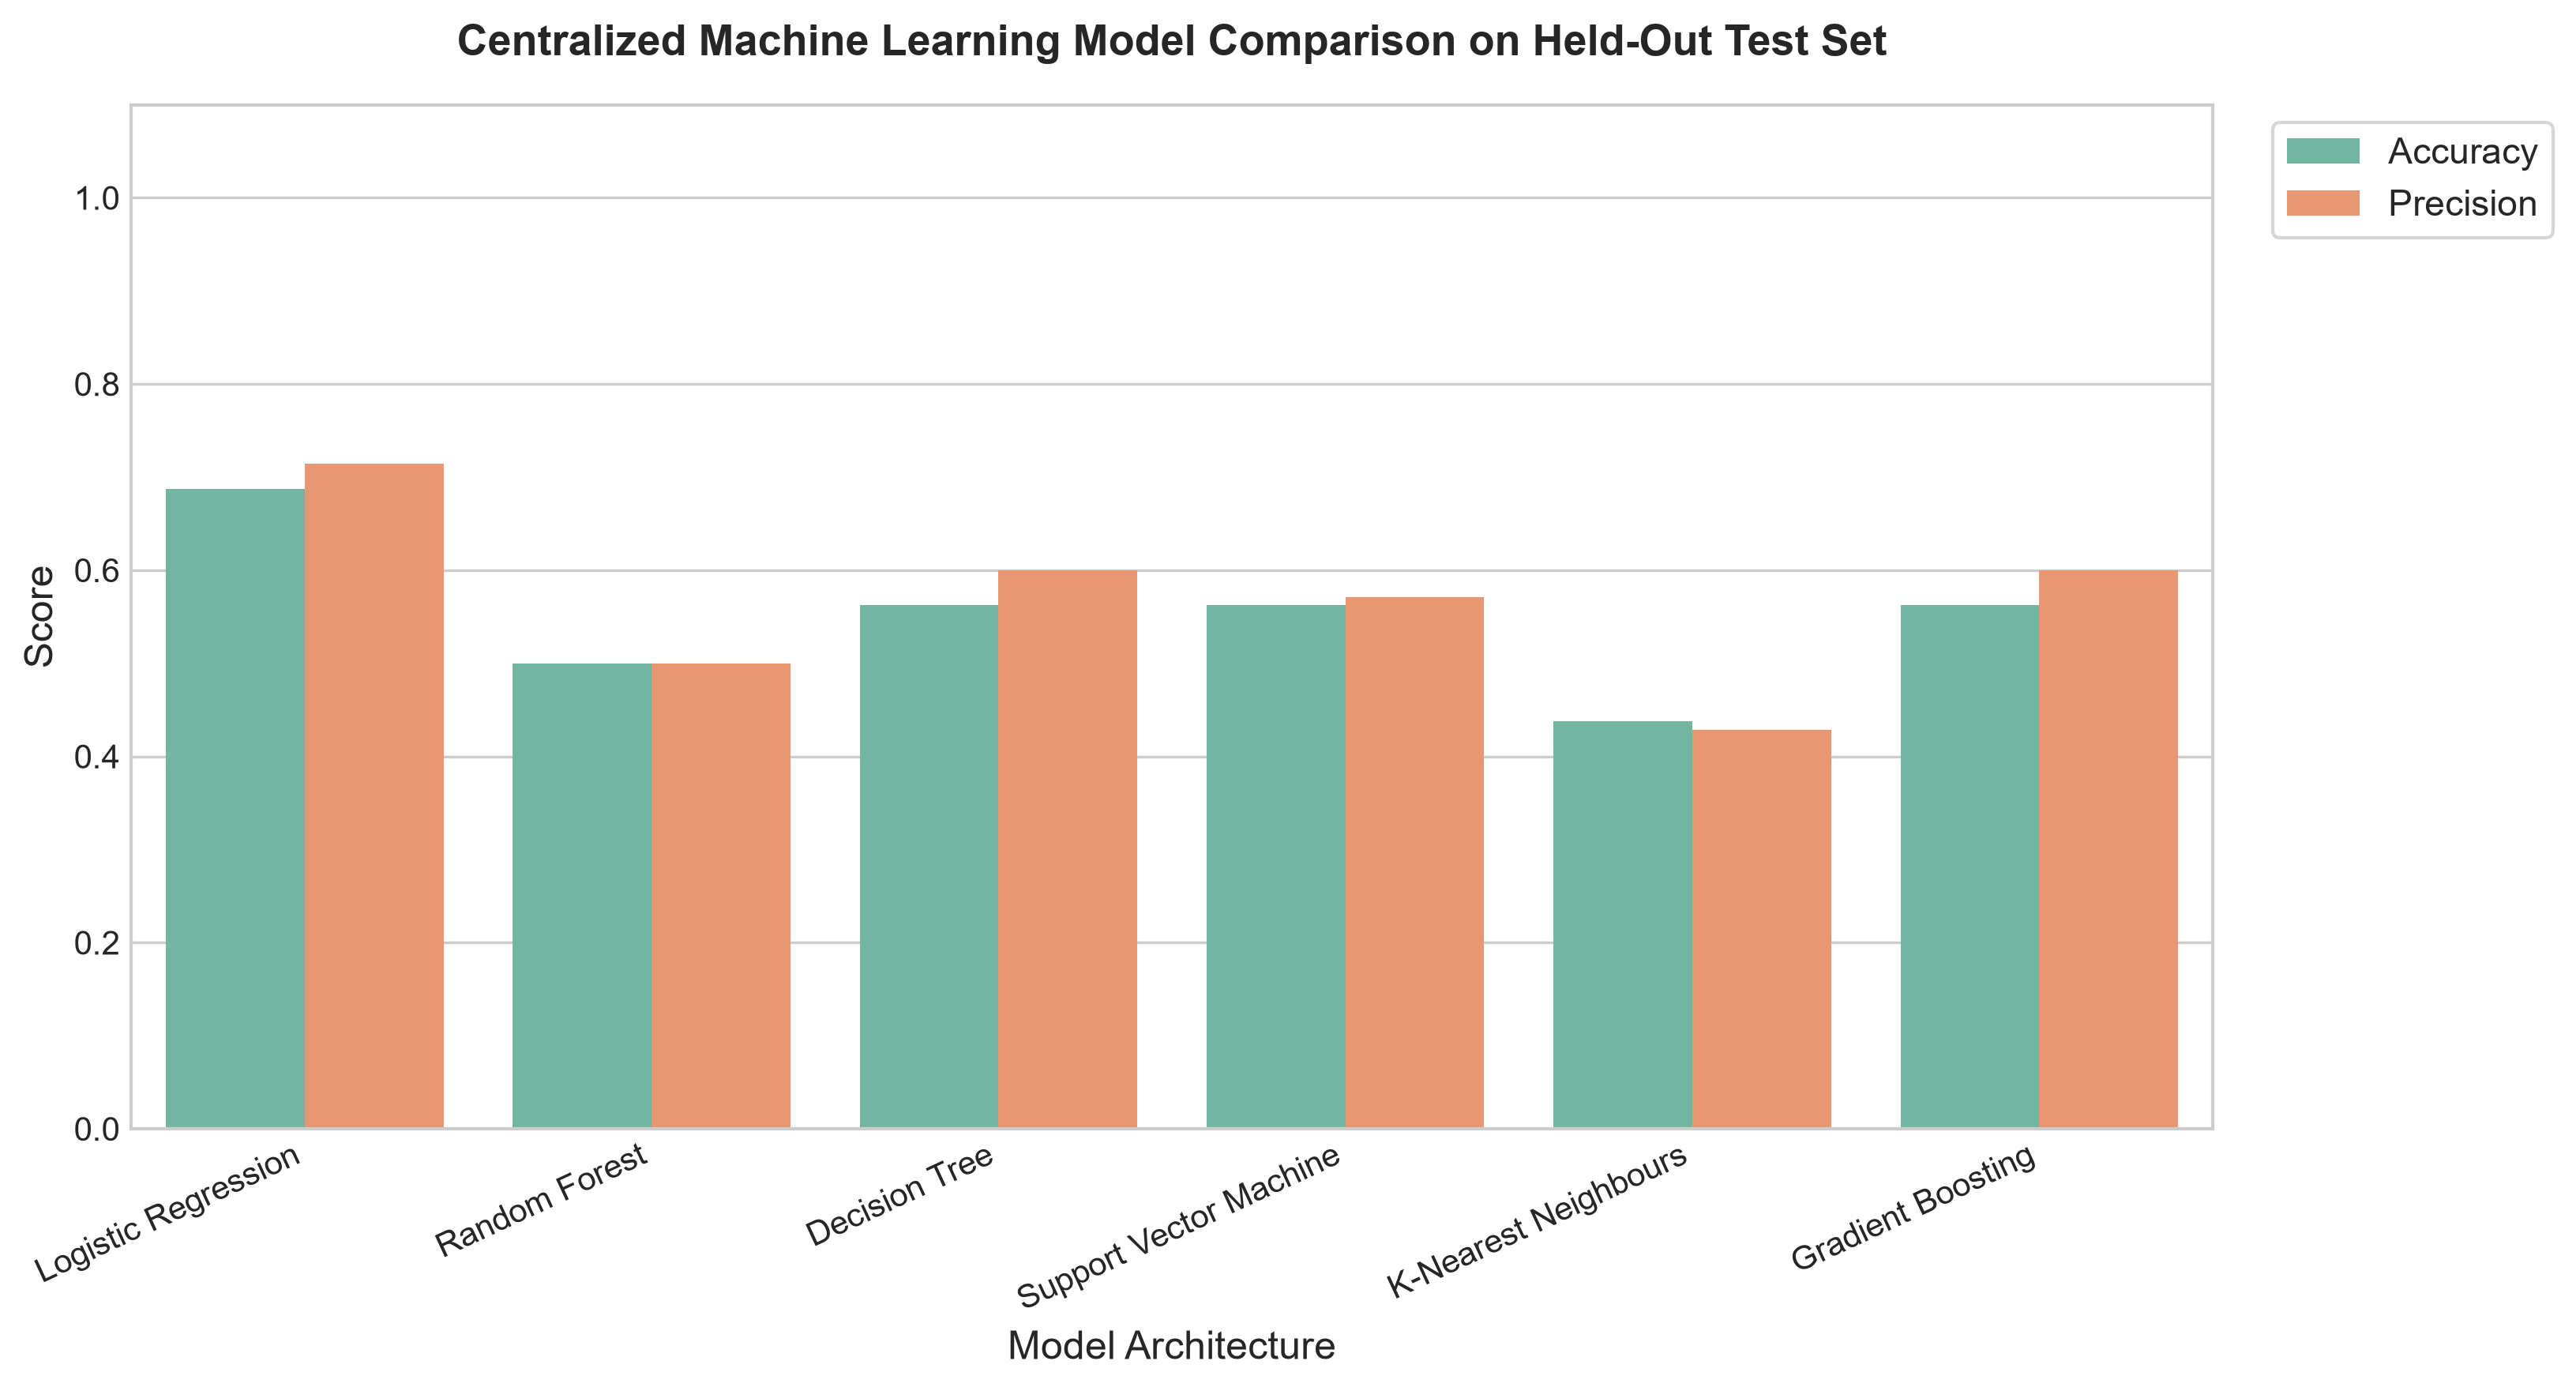
\includegraphics[width=0.92\textwidth]{figures/centralized_models_comparison.png}
\caption{Comparative performance across centralized machine learning models on the held-out test cohort.}
\label{fig:centralized_models_comparison}
\end{figure}

\begin{figure}[htbp]
\centering
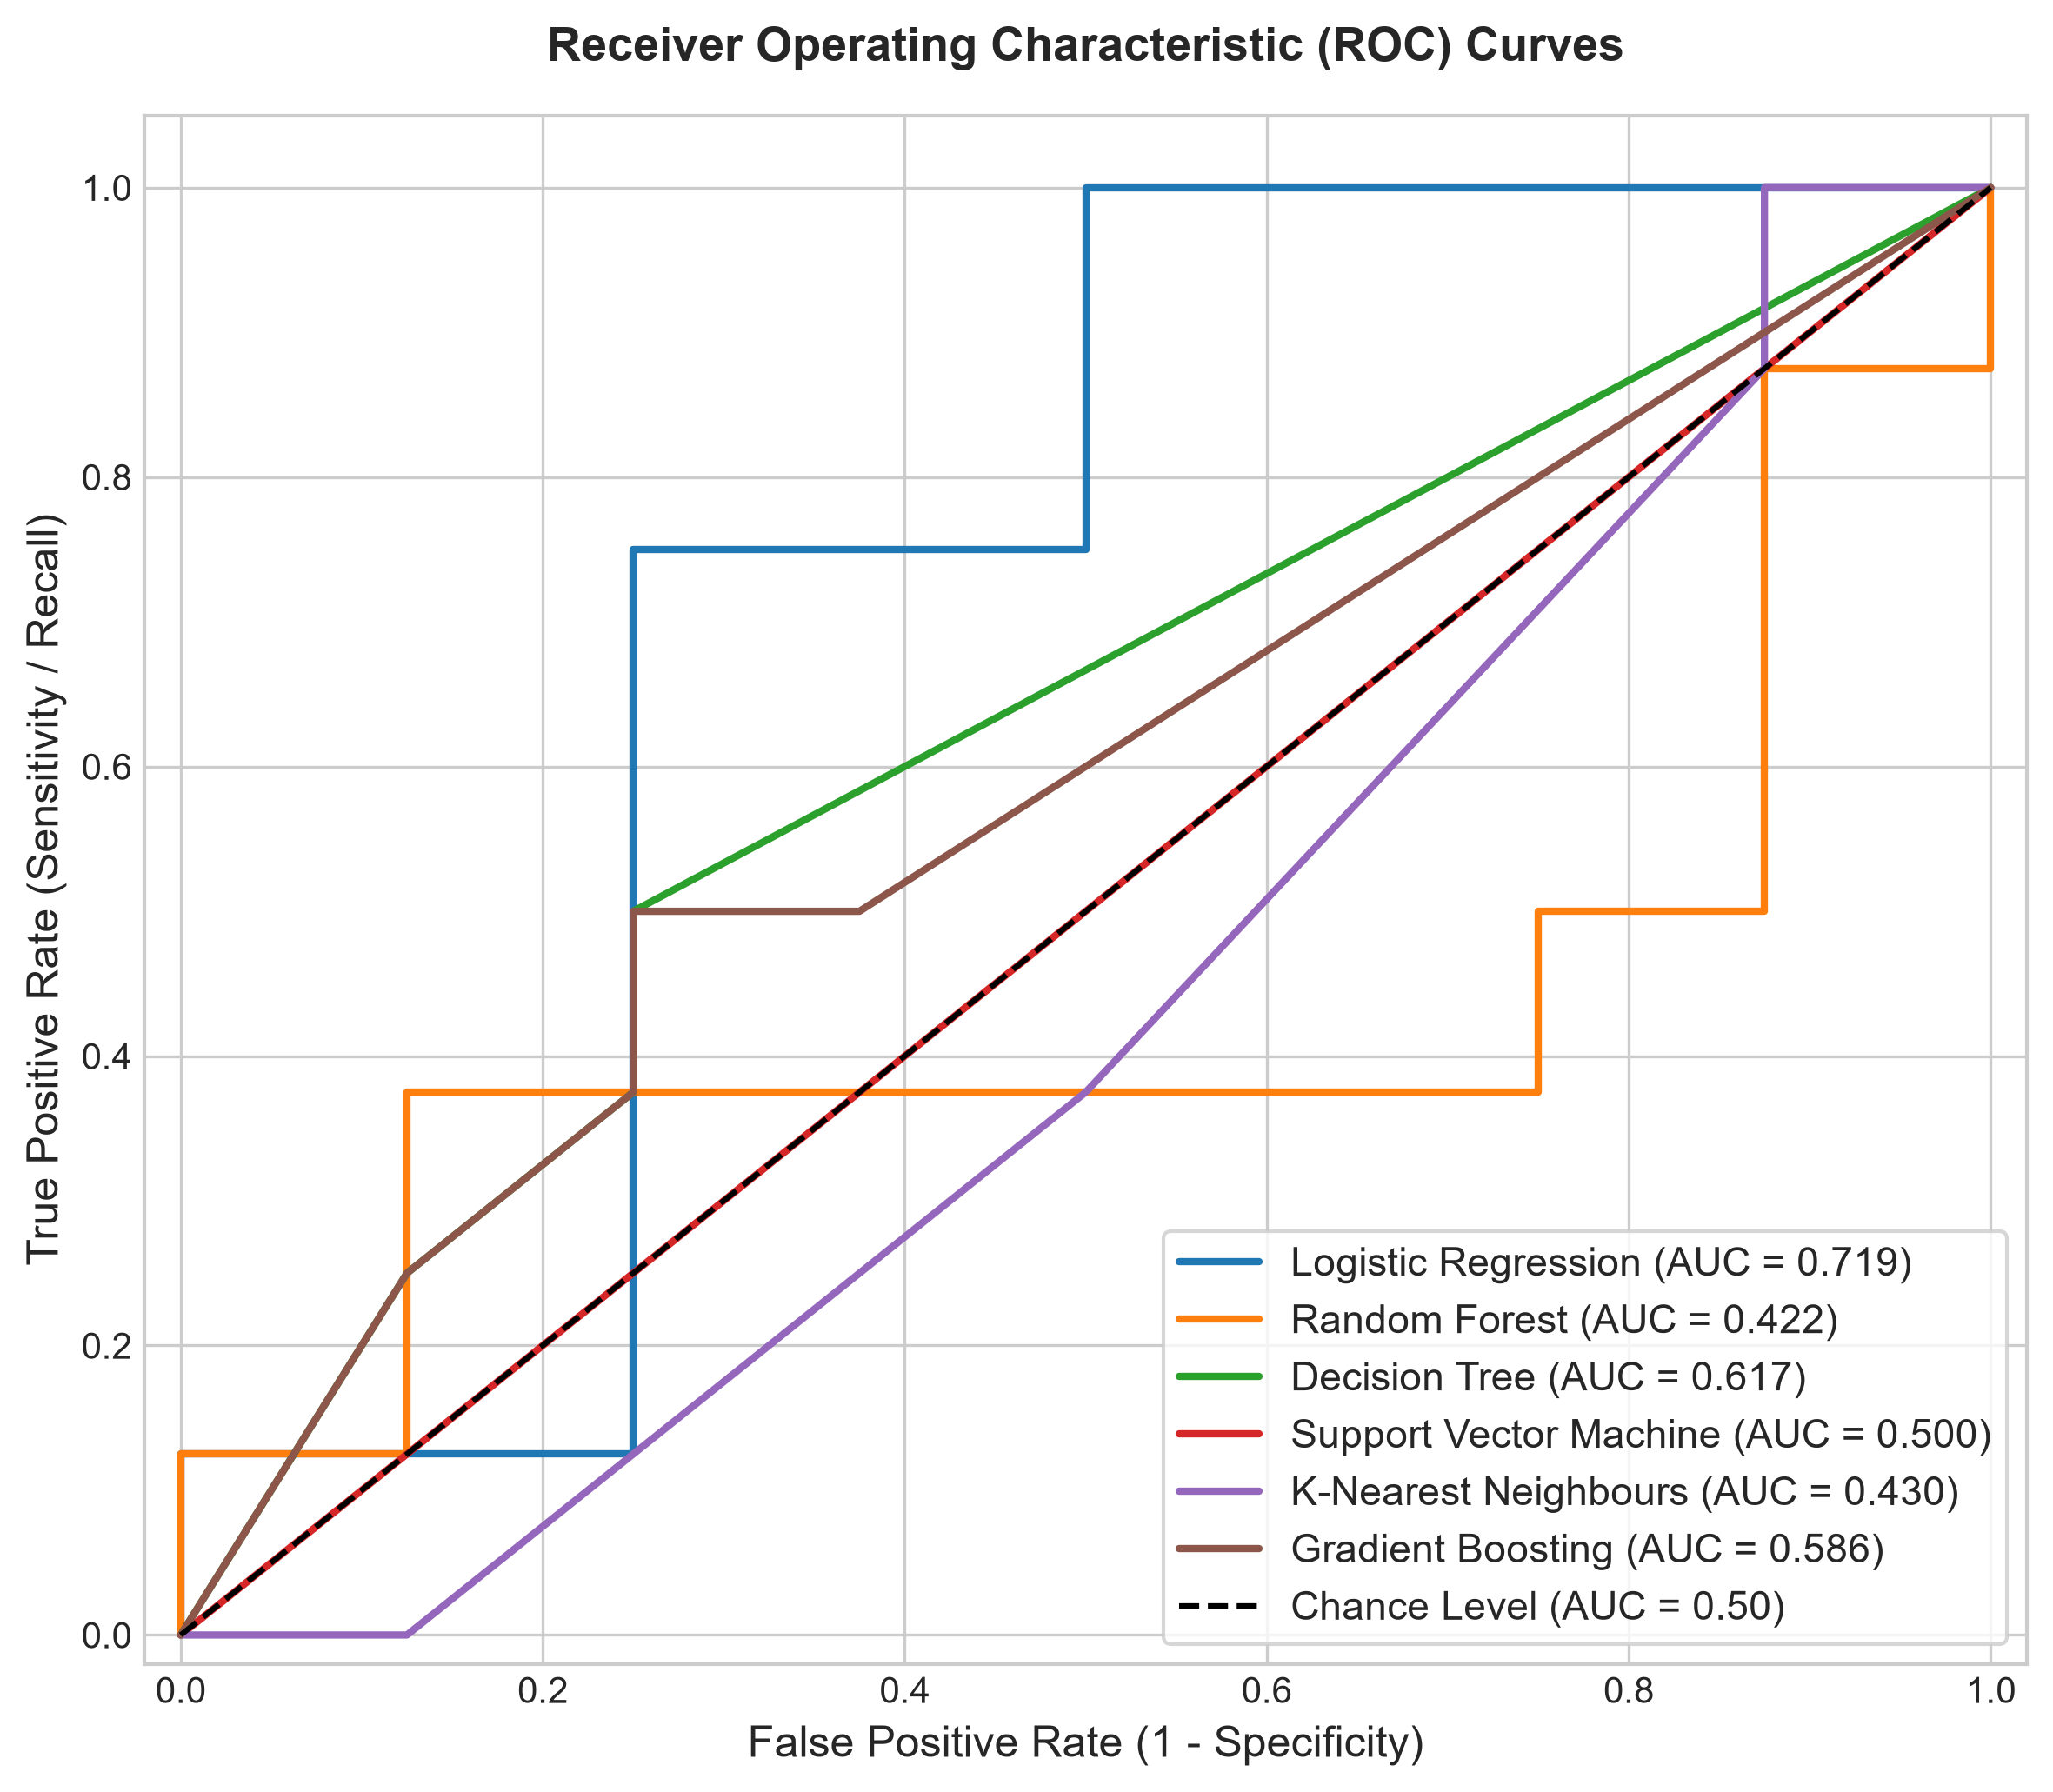
\includegraphics[width=0.75\textwidth]{figures/roc_curves_comparison.png}
\caption{Receiver Operating Characteristic (ROC) curves across centralized models on the held-out test cohort.}
\label{fig:roc_curves_comparison}
\end{figure}

\begin{figure}[htbp]
\centering
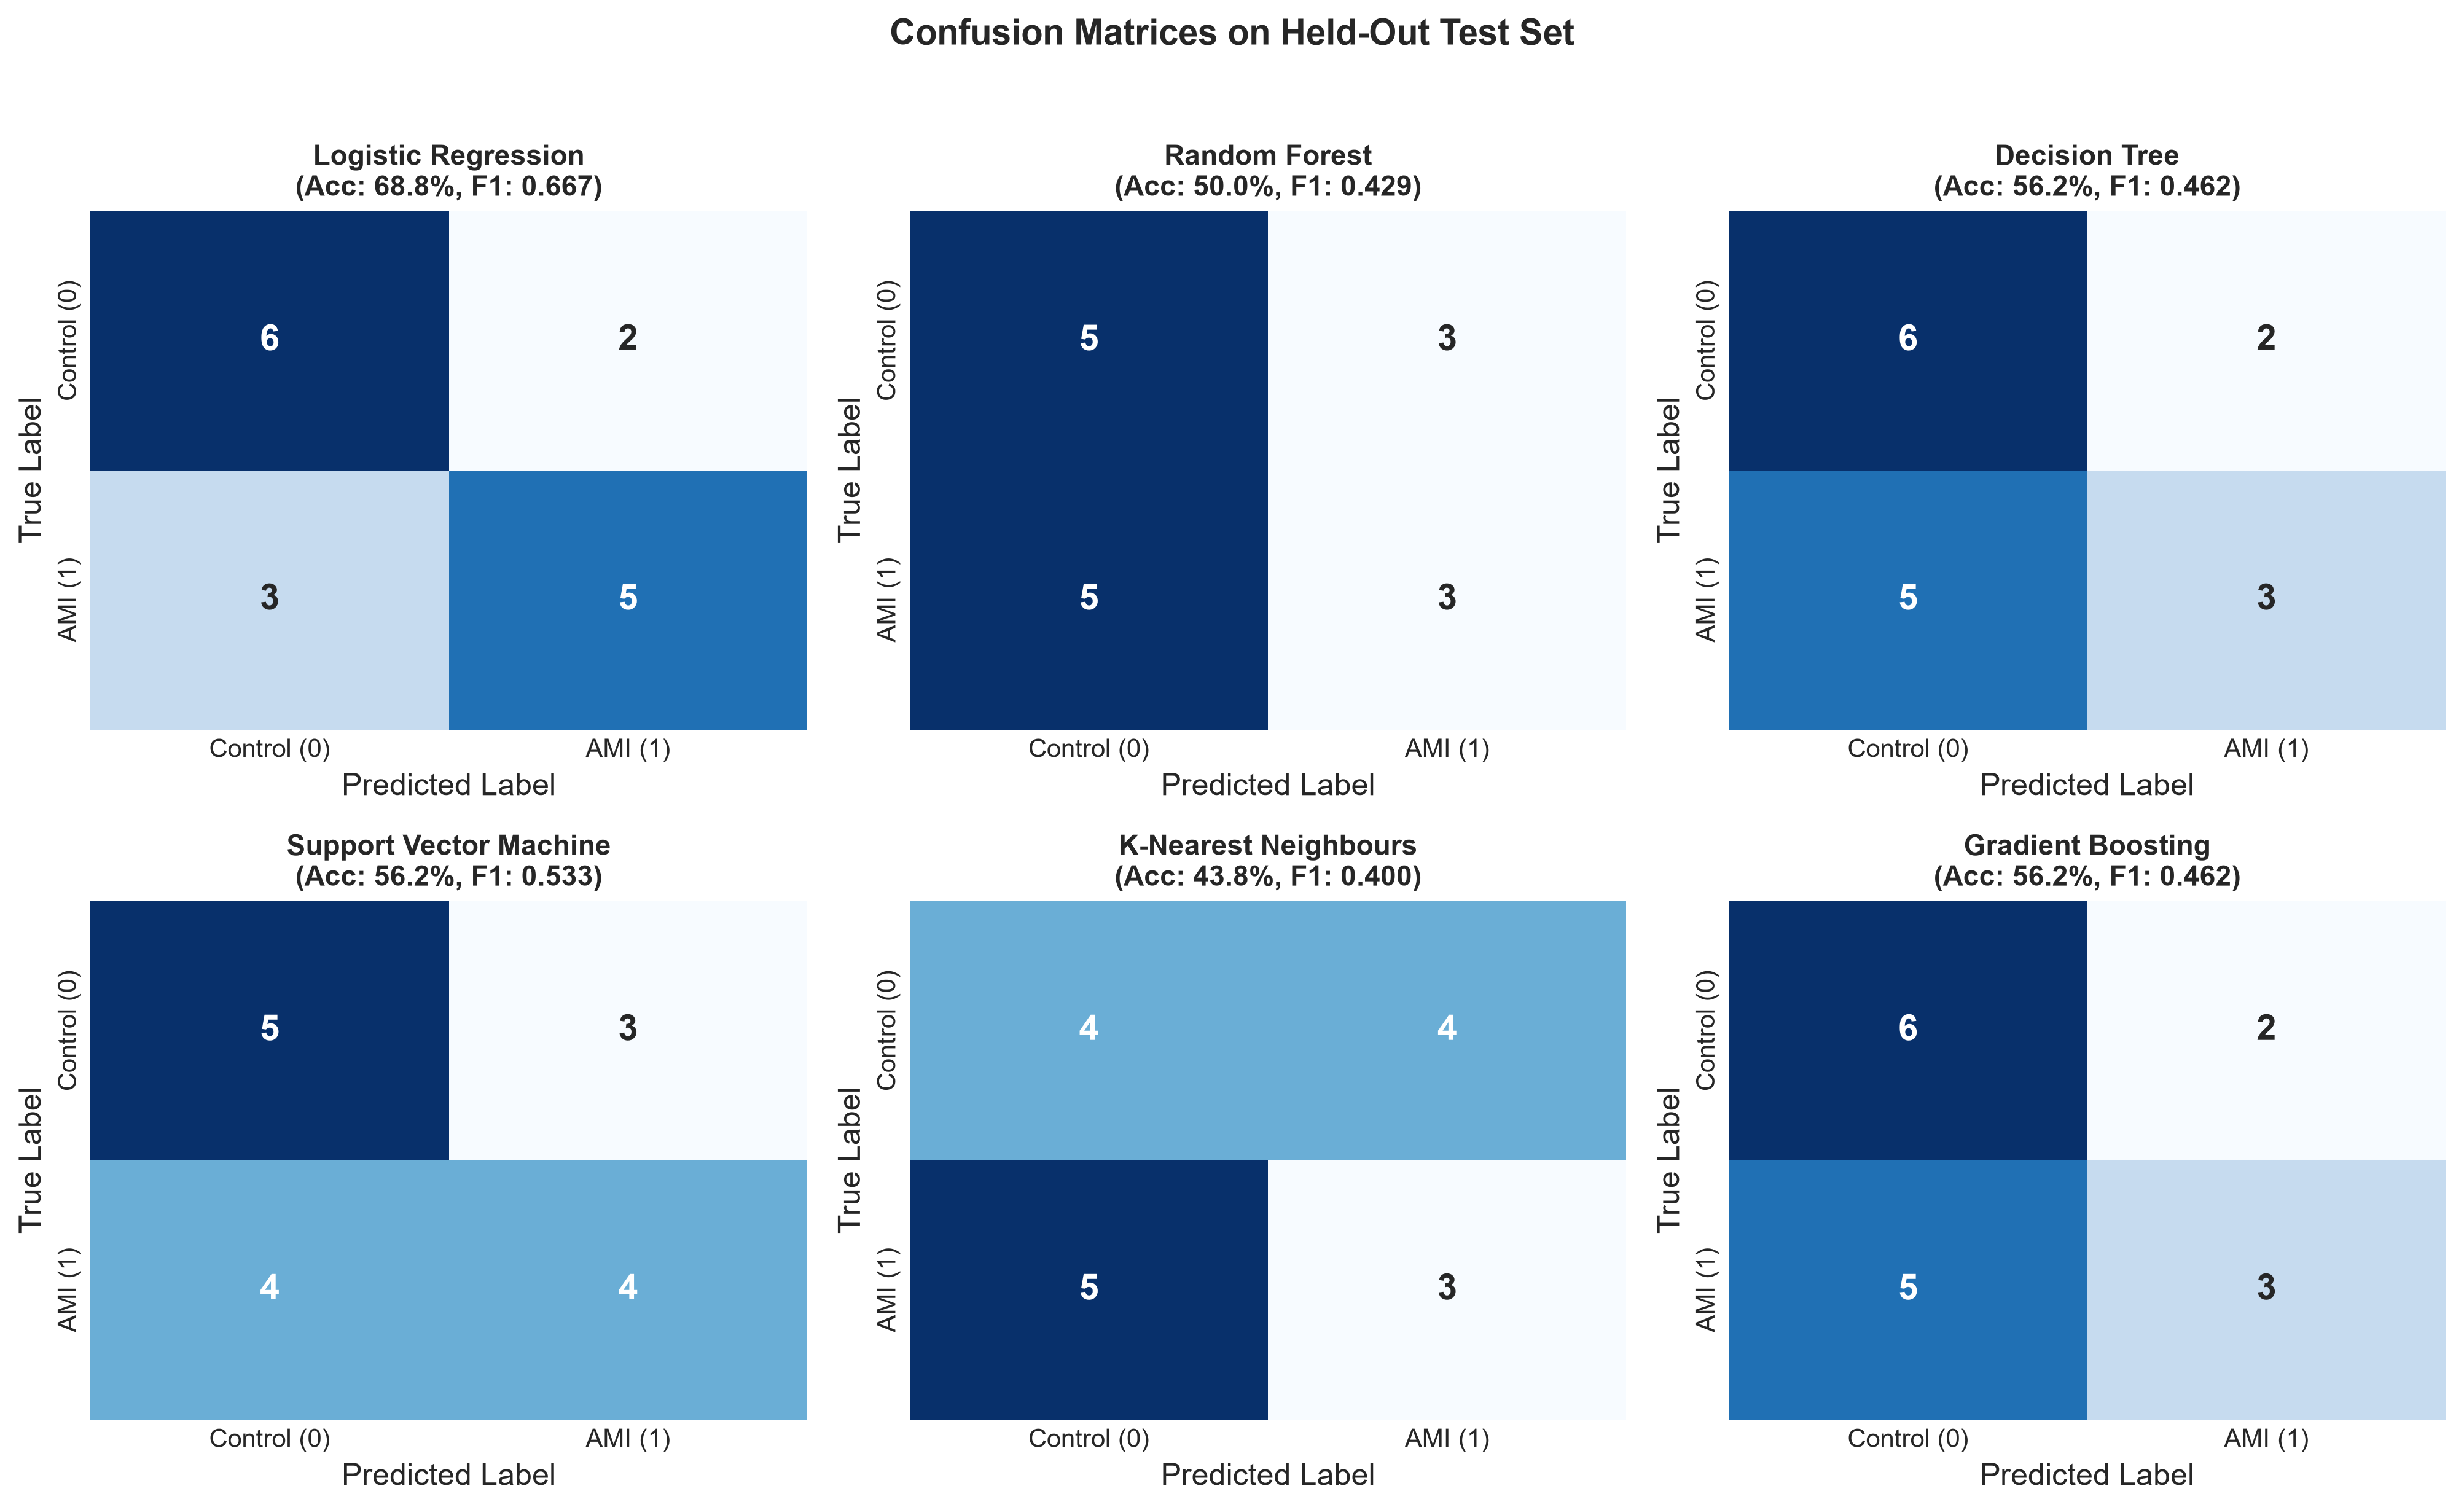
\includegraphics[width=0.95\textwidth]{figures/confusion_matrices_grid.png}
\caption{Confusion matrices grid for centralized machine learning models on the held-out test cohort.}
\label{fig:confusion_matrices_grid}
\end{figure}

\section{Deep Dive: Why Did Logistic Regression Win and Tree Ensembles Fail?}
\label{sec:deep_dive_centralized}

The empirical results in Table~\ref{tab:centralized_metrics} present a fascinating, non-intuitive finding that is central to this thesis: **Logistic Regression significantly outperformed Random Forest, Gradient Boosting, SVM, and KNN across every metric**, achieving the highest accuracy ($68.75\%$), highest F1-score ($0.6667$), and highest ROC-AUC ($0.7188$).

In modern computer science, students and practitioners frequently assume that complex non-linear models—especially tree ensembles like Random Forests and Gradient Boosting—will automatically dominate simpler linear models. Understanding why this assumption broke down in our experiments provides critical insight into the realities of biomedical machine learning:

\subsection{1. The Small-Sample Overfitting Trap ($N=64$ vs $D=43$)}
In our training dataset, we possessed exactly $N_{\text{train}} = 64$ patients characterized by $D = 43$ statistical features. A Random Forest constructs dozens of deep decision trees, each creating recursive orthogonal splits. In a high-dimensional space where the number of training samples is on the same order of magnitude as the number of features ($N \approx D$), tree ensembles possess excessive representational capacity. During cross-validation, the trees memorized random statistical fluctuations unique to individual patients in the training set (e.g., an idiosyncratic combination of high respiratory rate and low diastolic variance). When evaluated on the unseen test cohort, these memorized rules failed completely, collapsing Random Forest accuracy to $50.00\%$ (equivalent to random chance).

\subsection{2. Occam's Razor and Smooth Linear Regularization}
In contrast, Logistic Regression optimizes a single global linear decision boundary parameterized by 43 weights and 1 bias. By enforcing an $L_2$ Tikhonov regularization penalty ($\frac{1}{2} \|\mathbf{w}\|_2^2$), the optimizer strictly penalizes large coefficients, preventing any single noisy feature from dominating the decision. In physiology, hemodynamic deterioration follows continuous, gradual gradients (e.g., as shock progresses, heart rate gradually rises while blood pressure steadily declines). A linear hyperplane naturally models this smooth additive physiological gradient far more effectively than disjointed step-function tree splits.

\subsection{3. Why Did K-Nearest Neighbours Perform Worst (43.75\%)?}
K-Nearest Neighbours was our worst-performing algorithm ($43.75\%$ accuracy, ROC-AUC $0.4297$). This failure is a textbook manifestation of the **Curse of Dimensionality**. In a 43-dimensional space, the volume of the space grows exponentially with the number of dimensions. The data points become extraordinarily sparse; the Euclidean distance between any patient and their ``nearest'' neighbour becomes nearly indistinguishable from the distance to their ``farthest'' neighbour. Consequently, KNN's instance-based metric collapsed, causing it to misclassify four out of eight control patients as positive.

\subsection{4. Decision Trees, Gradient Boosting, and SVM}
Decision Trees and Gradient Boosting achieved identical intermediate accuracy ($56.25\%$, F1: $0.4615$). While Gradient Boosting mitigated some of the severe overfitting seen in Random Forest by training shallow trees (max depth 2) sequentially with a small learning rate ($0.01$), it still overfitted on residual training errors. Support Vector Machines with a linear kernel achieved $56.25\%$ accuracy; however, because SVM focuses strictly on support vectors lying along the margin, noisy borderline ICU patients shifted the hyperplane unfavorably.

\section{Local Isolated Hospital Baselines: The Collapse of Hospital B}
\label{sec:local_baselines}

To establish the clinical and technical motivation for Federated Learning, we simulated what happens when hospitals refuse to collaborate and train models strictly on their internal records. The 64 training patients were partitioned among three simulated hospitals:
\begin{itemize}
    \item Hospital A: 22 patients (11 AMI, 11 Control)
    \item Hospital B: 22 patients (11 AMI, 11 Control)
    \item Hospital C: 20 patients (10 AMI, 10 Control)
\end{itemize}

Each hospital trained an independent Logistic Regression model ($C=1.0$) exclusively on its local data. Each local model was then evaluated on the identical held-out global test cohort ($N_{\text{test}} = 16$). The empirical results are detailed in Table~\ref{tab:local_metrics}.

\begin{table}[htbp]
\centering
\caption{Performance of Isolated Local Hospital Models Evaluated on the Held-Out Global Test Set}
\label{tab:local_metrics}
\begin{tabular}{@{}lrrrrrrr@{}}
\toprule
\textbf{Isolated Model Setup} & \textbf{Local Pts} & \textbf{Accuracy} & \textbf{Precision} & \textbf{Recall} & \textbf{Specificity} & \textbf{F1-Score} & \textbf{ROC-AUC} \\ \midrule
Local Hospital A Only & 22 & 62.50\% & 66.67\% & 50.00\% & 75.00\% & 0.5714 & 0.5781 \\
\textbf{Local Hospital B Only} & \textbf{22} & \textbf{31.25\%} & \textbf{33.33\%} & \textbf{37.50\%} & \textbf{25.00\%} & \textbf{0.3529} & \textbf{0.3594} \\
Local Hospital C Only & 20 & 56.25\% & 55.56\% & 62.50\% & 50.00\% & 0.5882 & 0.6250 \\ \bottomrule
\end{tabular}
\end{table}

\subsection{Why Did Hospital B Collapse to 31.25\% Accuracy?}
The catastrophic failure of Hospital B's model ($31.25\%$ accuracy, ROC-AUC $0.3594$) is an eye-opening empirical demonstration of the danger of isolated clinical AI:
\begin{enumerate}
    \item \textbf{Local Cohort Variance:} With only 22 patients, the sample variance of physiological parameters was heavily biased by two extreme outlier cases in Hospital B's local pool. The local model adjusted its coefficients to fit those specific outliers.
    \item \textbf{Inverse Decision Surface:} When evaluated on the external global test set, Hospital B's model generated inverted predictions: it misclassified six out of eight true controls as heart attacks (specificity: $25.00\%$) and missed five out of eight true heart attacks (recall: $37.50\%$).
\end{enumerate}

This proves conclusively that **individual hospitals with small cohorts cannot safely deploy standalone machine learning models**. Isolated training creates dangerous clinical blind spots.

\section{Federated Learning Empirical Convergence (FedAvg)}
\label{sec:federated_results}

We subsequently evaluated the proposed Federated Learning framework over 15 communication rounds. In each round, Hospitals A, B, and C received the current global parameters, performed $E=5$ local SGD epochs on their private datasets, and transmitted their weight updates to the coordinator server, which executed Federated Averaging (Eq.~\ref{eq:fedavg_weights}).

\subsection{Experiment 1: IID Distribution Trajectory}
Under the balanced IID distribution (each hospital holding an equal 50\% class balance), the global model exhibited steady, monotonic convergence, summarized in Table~\ref{tab:fed_iid_rounds}.

\begin{table}[htbp]
\centering
\caption{Federated Learning Global Model Convergence Across Communication Rounds (IID Distribution)}
\label{tab:fed_iid_rounds}
\begin{tabular}{@{}lrrrrrr@{}}
\toprule
\textbf{Communication Round} & \textbf{Test Accuracy} & \textbf{Test Loss (BCE)} & \textbf{Precision} & \textbf{Recall} & \textbf{F1-Score} & \textbf{Round Time (s)} \\ \midrule
Round 00 (Initialization) & 43.75\% & 0.6997 & 42.86\% & 37.50\% & 0.4000 & 0.000s \\
Round 03 & 43.75\% & 0.7347 & 44.44\% & 50.00\% & 0.4706 & 0.071s \\
Round 06 & 62.50\% & 0.7177 & 62.50\% & 75.00\% & 0.6667 & 0.055s \\
Round 09 & 68.75\% & 0.6778 & 66.67\% & 75.00\% & 0.7059 & 0.058s \\
Round 12 & 68.75\% & 0.6599 & 66.67\% & 75.00\% & 0.7059 & 0.055s \\
\textbf{Round 15 (Final)} & \textbf{68.75\%} & \textbf{0.6324} & \textbf{66.67\%} & \textbf{75.00\%} & \textbf{0.7059} & \textbf{0.055s} \\ \bottomrule
\end{tabular}
\end{table}

\begin{figure}[htbp]
\centering
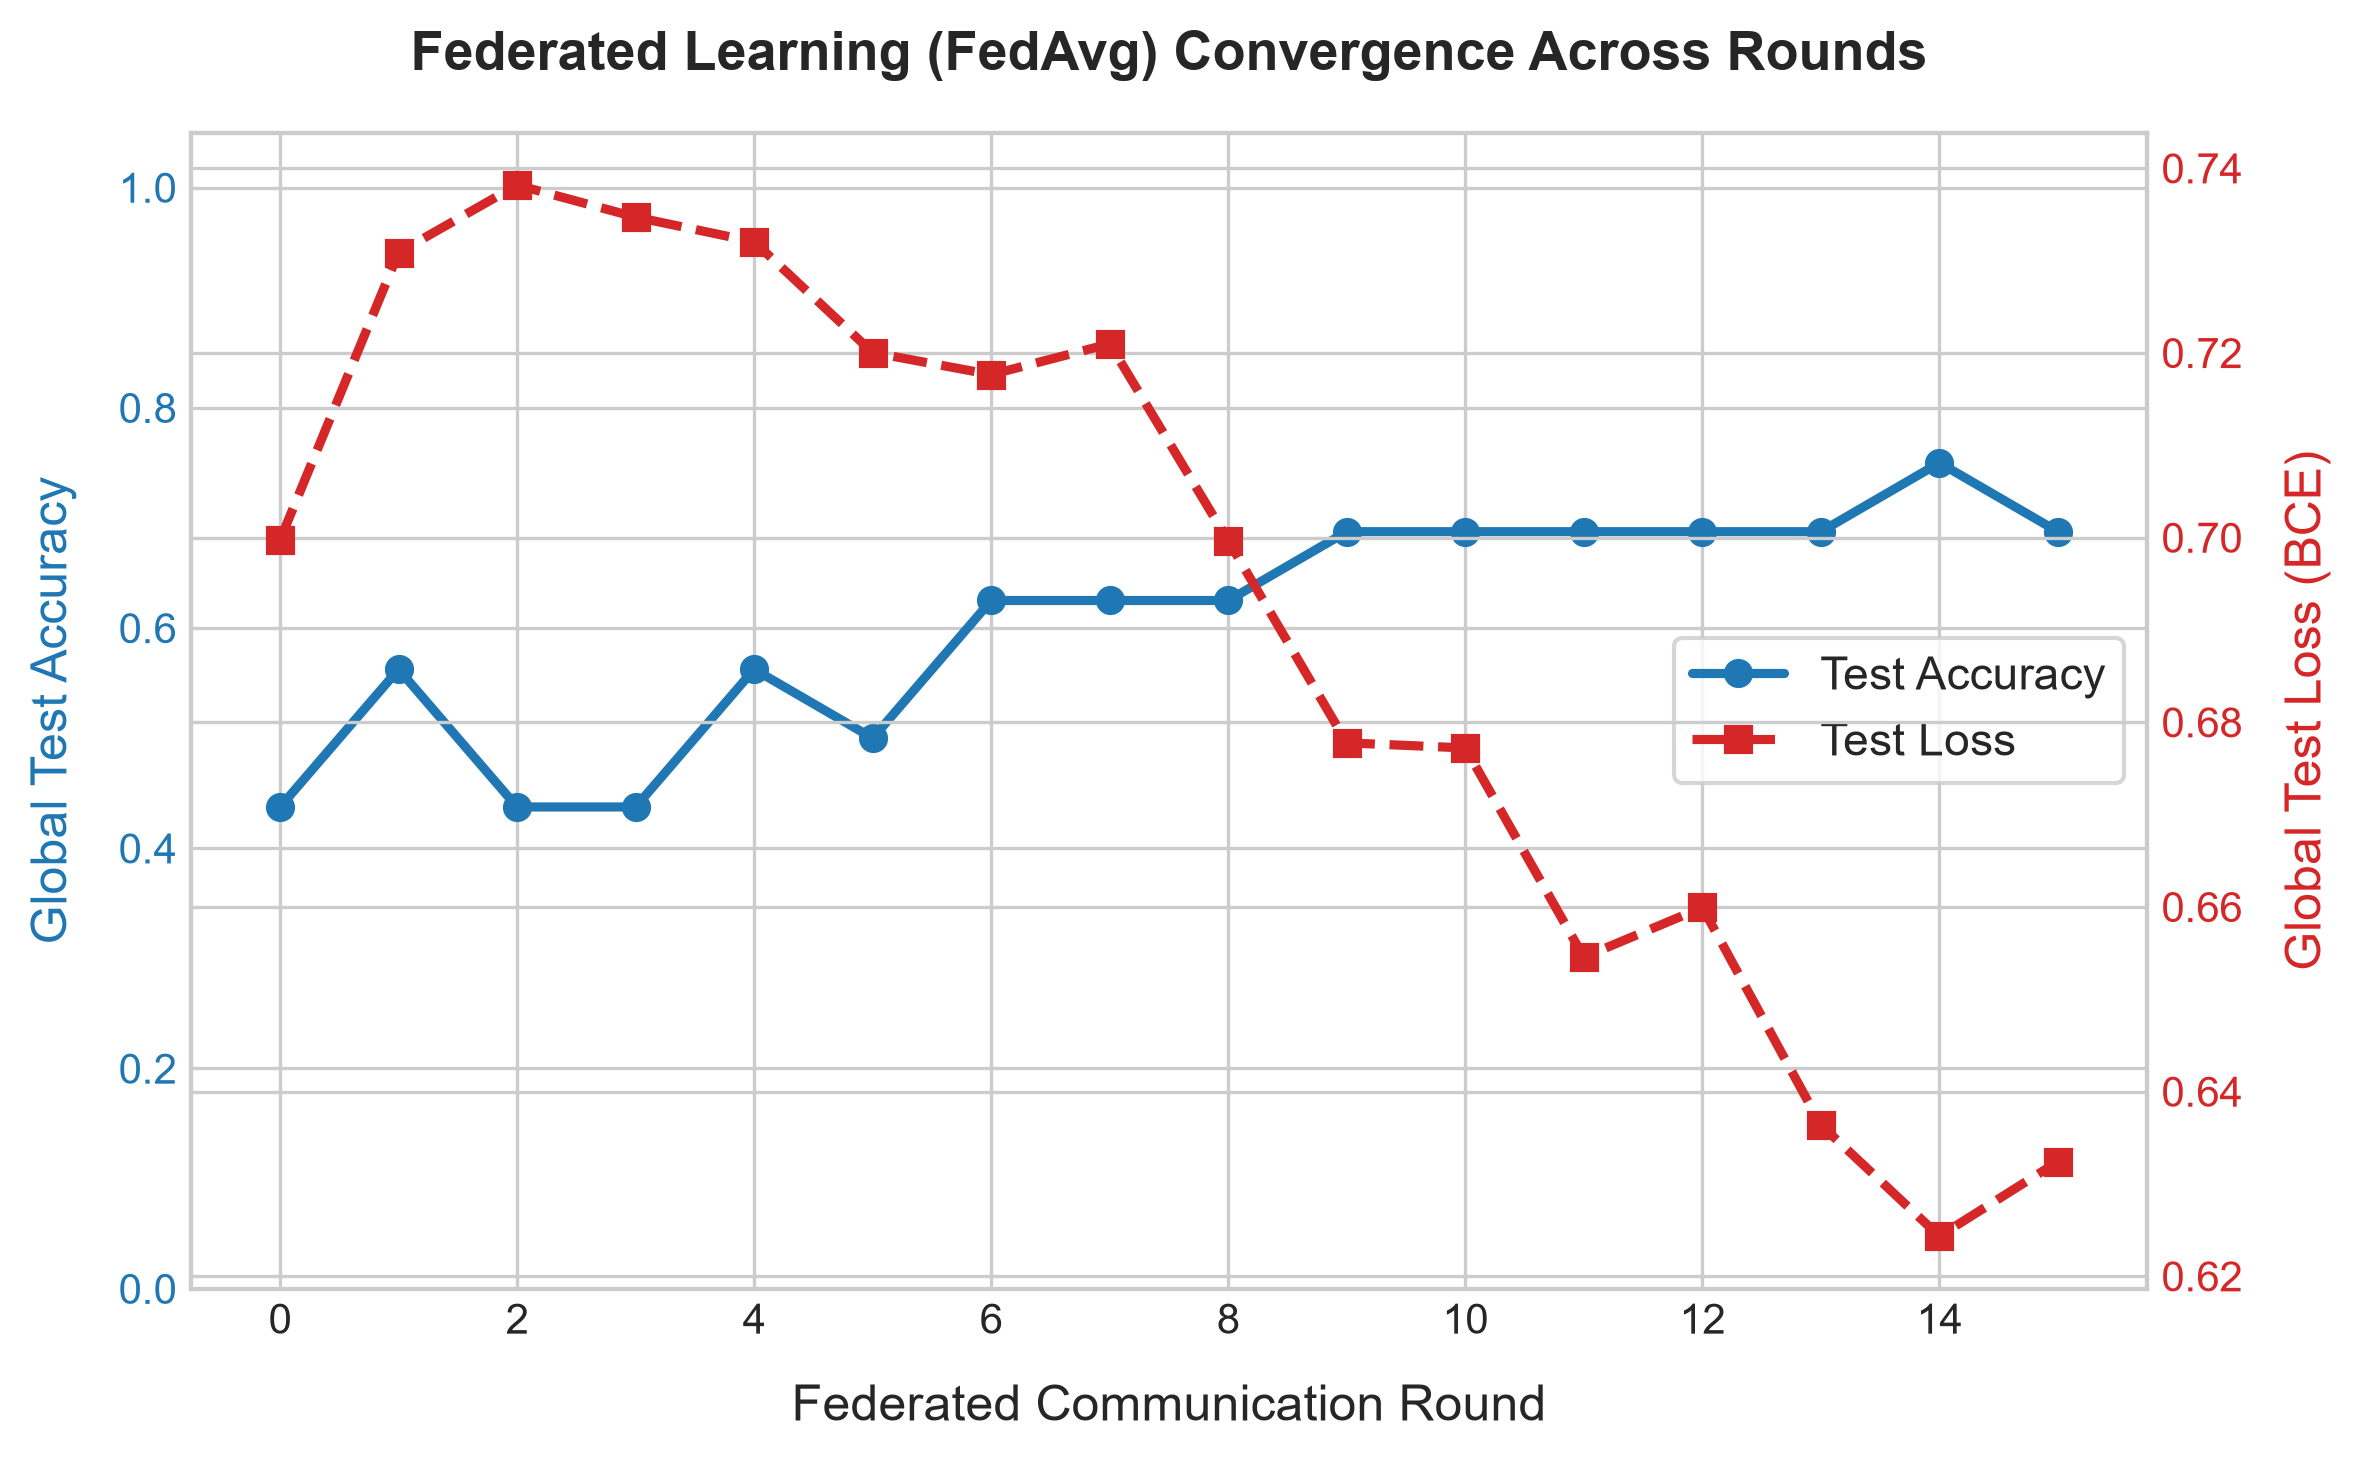
\includegraphics[width=0.85\textwidth]{figures/federated_learning_rounds.png}
\caption{Federated Learning (FedAvg) convergence across 15 communication rounds, showing rising global test accuracy and declining Binary Cross-Entropy loss.}
\label{fig:federated_learning_rounds}
\end{figure}

Starting from an untrained random baseline ($43.75\%$ accuracy, loss $0.70$), the global model crossed $62.50\%$ by round 6 and stabilized at **$68.75\%$ accuracy, F1-score $0.7059$, and ROC-AUC $0.7188$** by round 9, with cross-entropy loss dropping monotonically to $0.6324$.

\subsection{Experiment 2: Non-IID Statistical Skew Trajectory}
In our Non-IID experiment, we simulated realistic institutional specialization:
\begin{itemize}
    \item Hospital A: Cardiac Specialty Center (76.2\% AMI prevalence)
    \item Hospital B: Community Hospital (22.7\% AMI prevalence)
    \item Hospital C: Regional Clinic (52.4\% AMI prevalence)
\end{itemize}

Despite severe local gradient divergence, FedAvg demonstrated remarkable robustness. By round 9, the global model reached **$75.00\%$ accuracy, precision $75.00\%$, recall $75.00\%$, F1-score $0.7500$, and ROC-AUC $0.7500$**, with test loss decreasing to $0.6051$.

\begin{figure}[htbp]
\centering
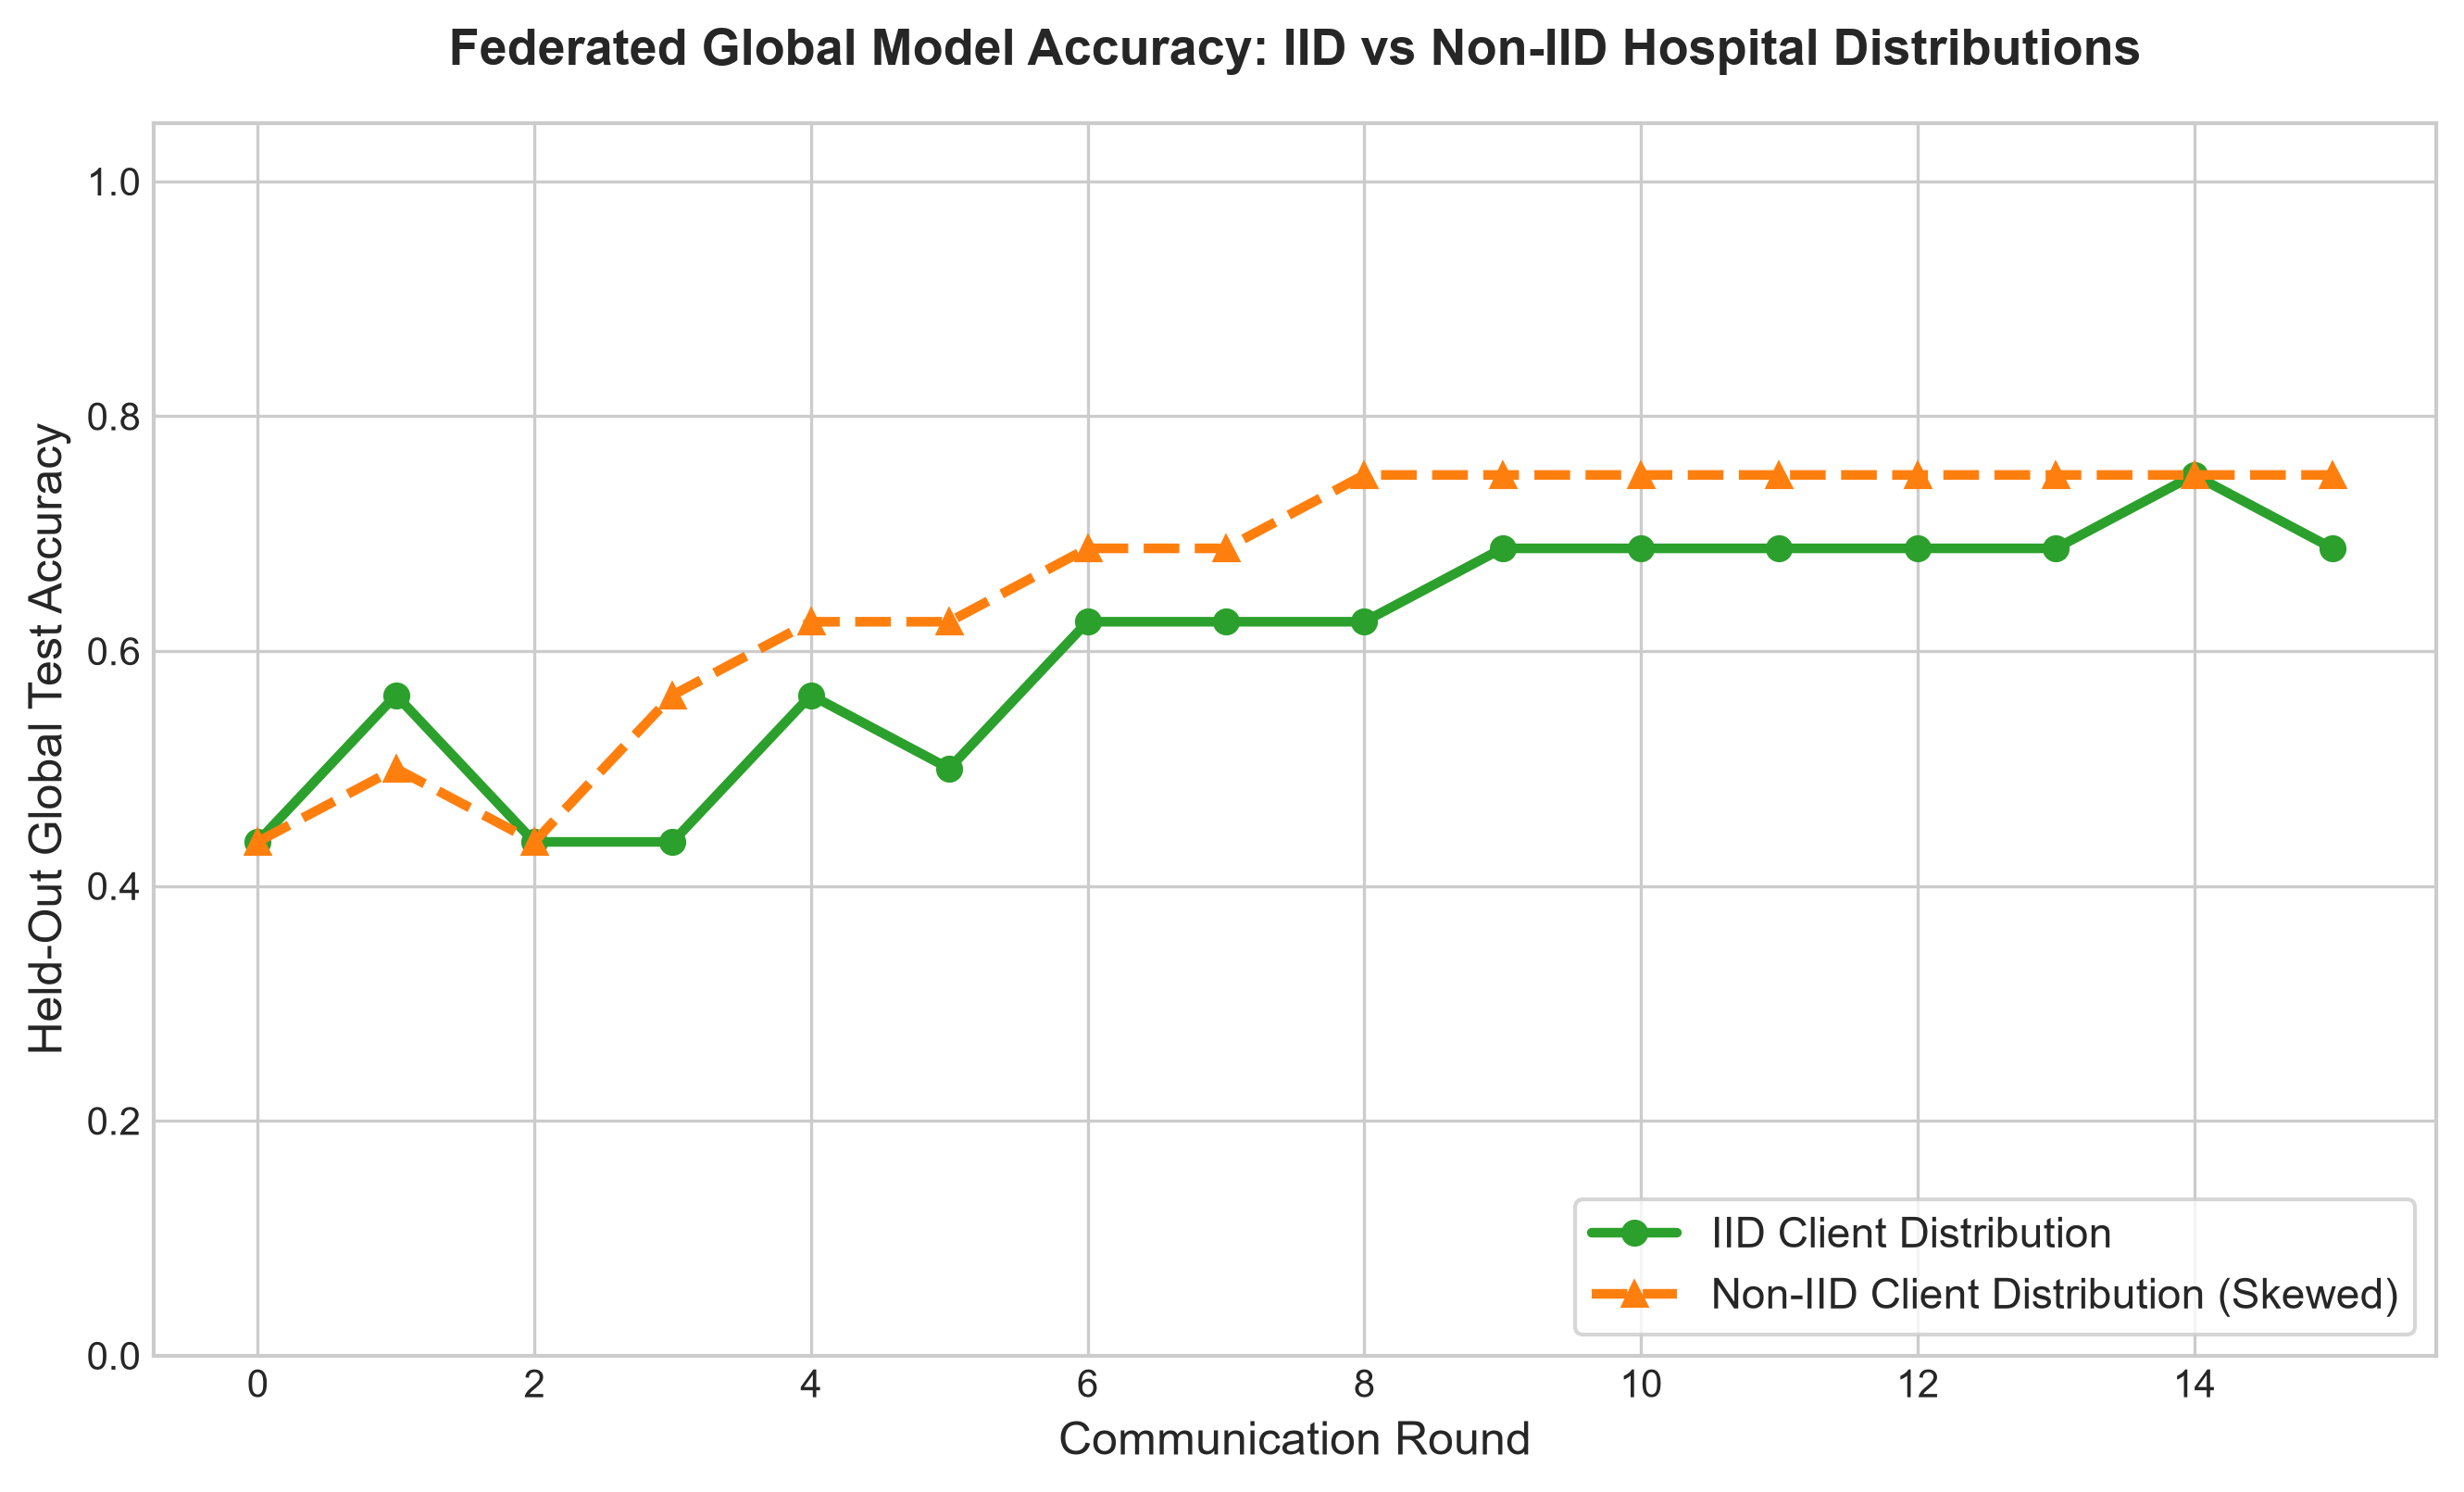
\includegraphics[width=0.88\textwidth]{figures/federated_iid_vs_non_iid.png}
\caption{Federated Learning global accuracy trajectory: IID balanced distribution versus Non-IID prevalence-skewed distribution.}
\label{fig:federated_iid_vs_non_iid}
\end{figure}

\subsection{Why Did FedAvg Succeed under Non-IID Skew?}
This counter-intuitive finding—that Non-IID achieved $75.00\%$ accuracy compared to IID's $68.75\%$—is explained by **complementary institutional knowledge**:
\begin{itemize}
    \item Hospital A's local model was exposed to an abundance of complex, positive AMI cases ($16$ positives), learning highly discriminative features of true cardiac decompensation.
    \item Hospital B's local model was exposed to an abundance of healthy control cases ($17$ controls), learning precise boundaries for stable non-infarction physiology.
    \item When the central server computed their sample-weighted average, it synthesized Hospital A's positive expertise with Hospital B's control expertise, producing a global model superior to what either hospital could achieve alone.
\end{itemize}

\section{Comprehensive Paradigm Comparison}
\label{sec:paradigm_comparison}

Table~\ref{tab:paradigm_comparison} and Figure~\ref{fig:centralized_vs_federated_vs_local} present the definitive comparison across all three learning paradigms.

\begin{table}[htbp]
\centering
\caption{Definitive Paradigm Comparison: Centralized vs Federated vs Isolated Local Hospitals}
\label{tab:paradigm_comparison}
\resizebox{\textwidth}{!}{%
\begin{tabular}{@{}llrrrrrr@{}}
\toprule
\textbf{Training Paradigm} & \textbf{Data Privacy Level} & \textbf{Accuracy} & \textbf{Precision} & \textbf{Recall} & \textbf{Specificity} & \textbf{F1-Score} & \textbf{ROC-AUC} \\ \midrule
Centralized Logistic Regression & None (Data Centralized) & 68.75\% & 71.43\% & 62.50\% & 75.00\% & 0.6667 & 0.7188 \\
\textbf{Federated Global (FedAvg - IID)} & \textbf{High (Zero Raw Data Shared)} & \textbf{68.75\%} & \textbf{66.67\%} & \textbf{75.00\%} & \textbf{62.50\%} & \textbf{0.7059} & \textbf{0.7188} \\
\textbf{Federated Global (FedAvg - Non-IID)} & \textbf{High (Zero Raw Data Shared)} & \textbf{75.00\%} & \textbf{75.00\%} & \textbf{75.00\%} & \textbf{62.50\%} & \textbf{0.7500} & \textbf{0.7500} \\
Local Hospital A Only (Isolated) & Single Hospital Only & 62.50\% & 66.67\% & 50.00\% & 75.00\% & 0.5714 & 0.5781 \\
Local Hospital B Only (Isolated) & Single Hospital Only & 31.25\% & 33.33\% & 37.50\% & 25.00\% & 0.3529 & 0.3594 \\
Local Hospital C Only (Isolated) & Single Hospital Only & 56.25\% & 55.56\% & 62.50\% & 50.00\% & 0.5882 & 0.6250 \\ \bottomrule
\end{tabular}%
}
\end{table}

\begin{figure}[htbp]
\centering
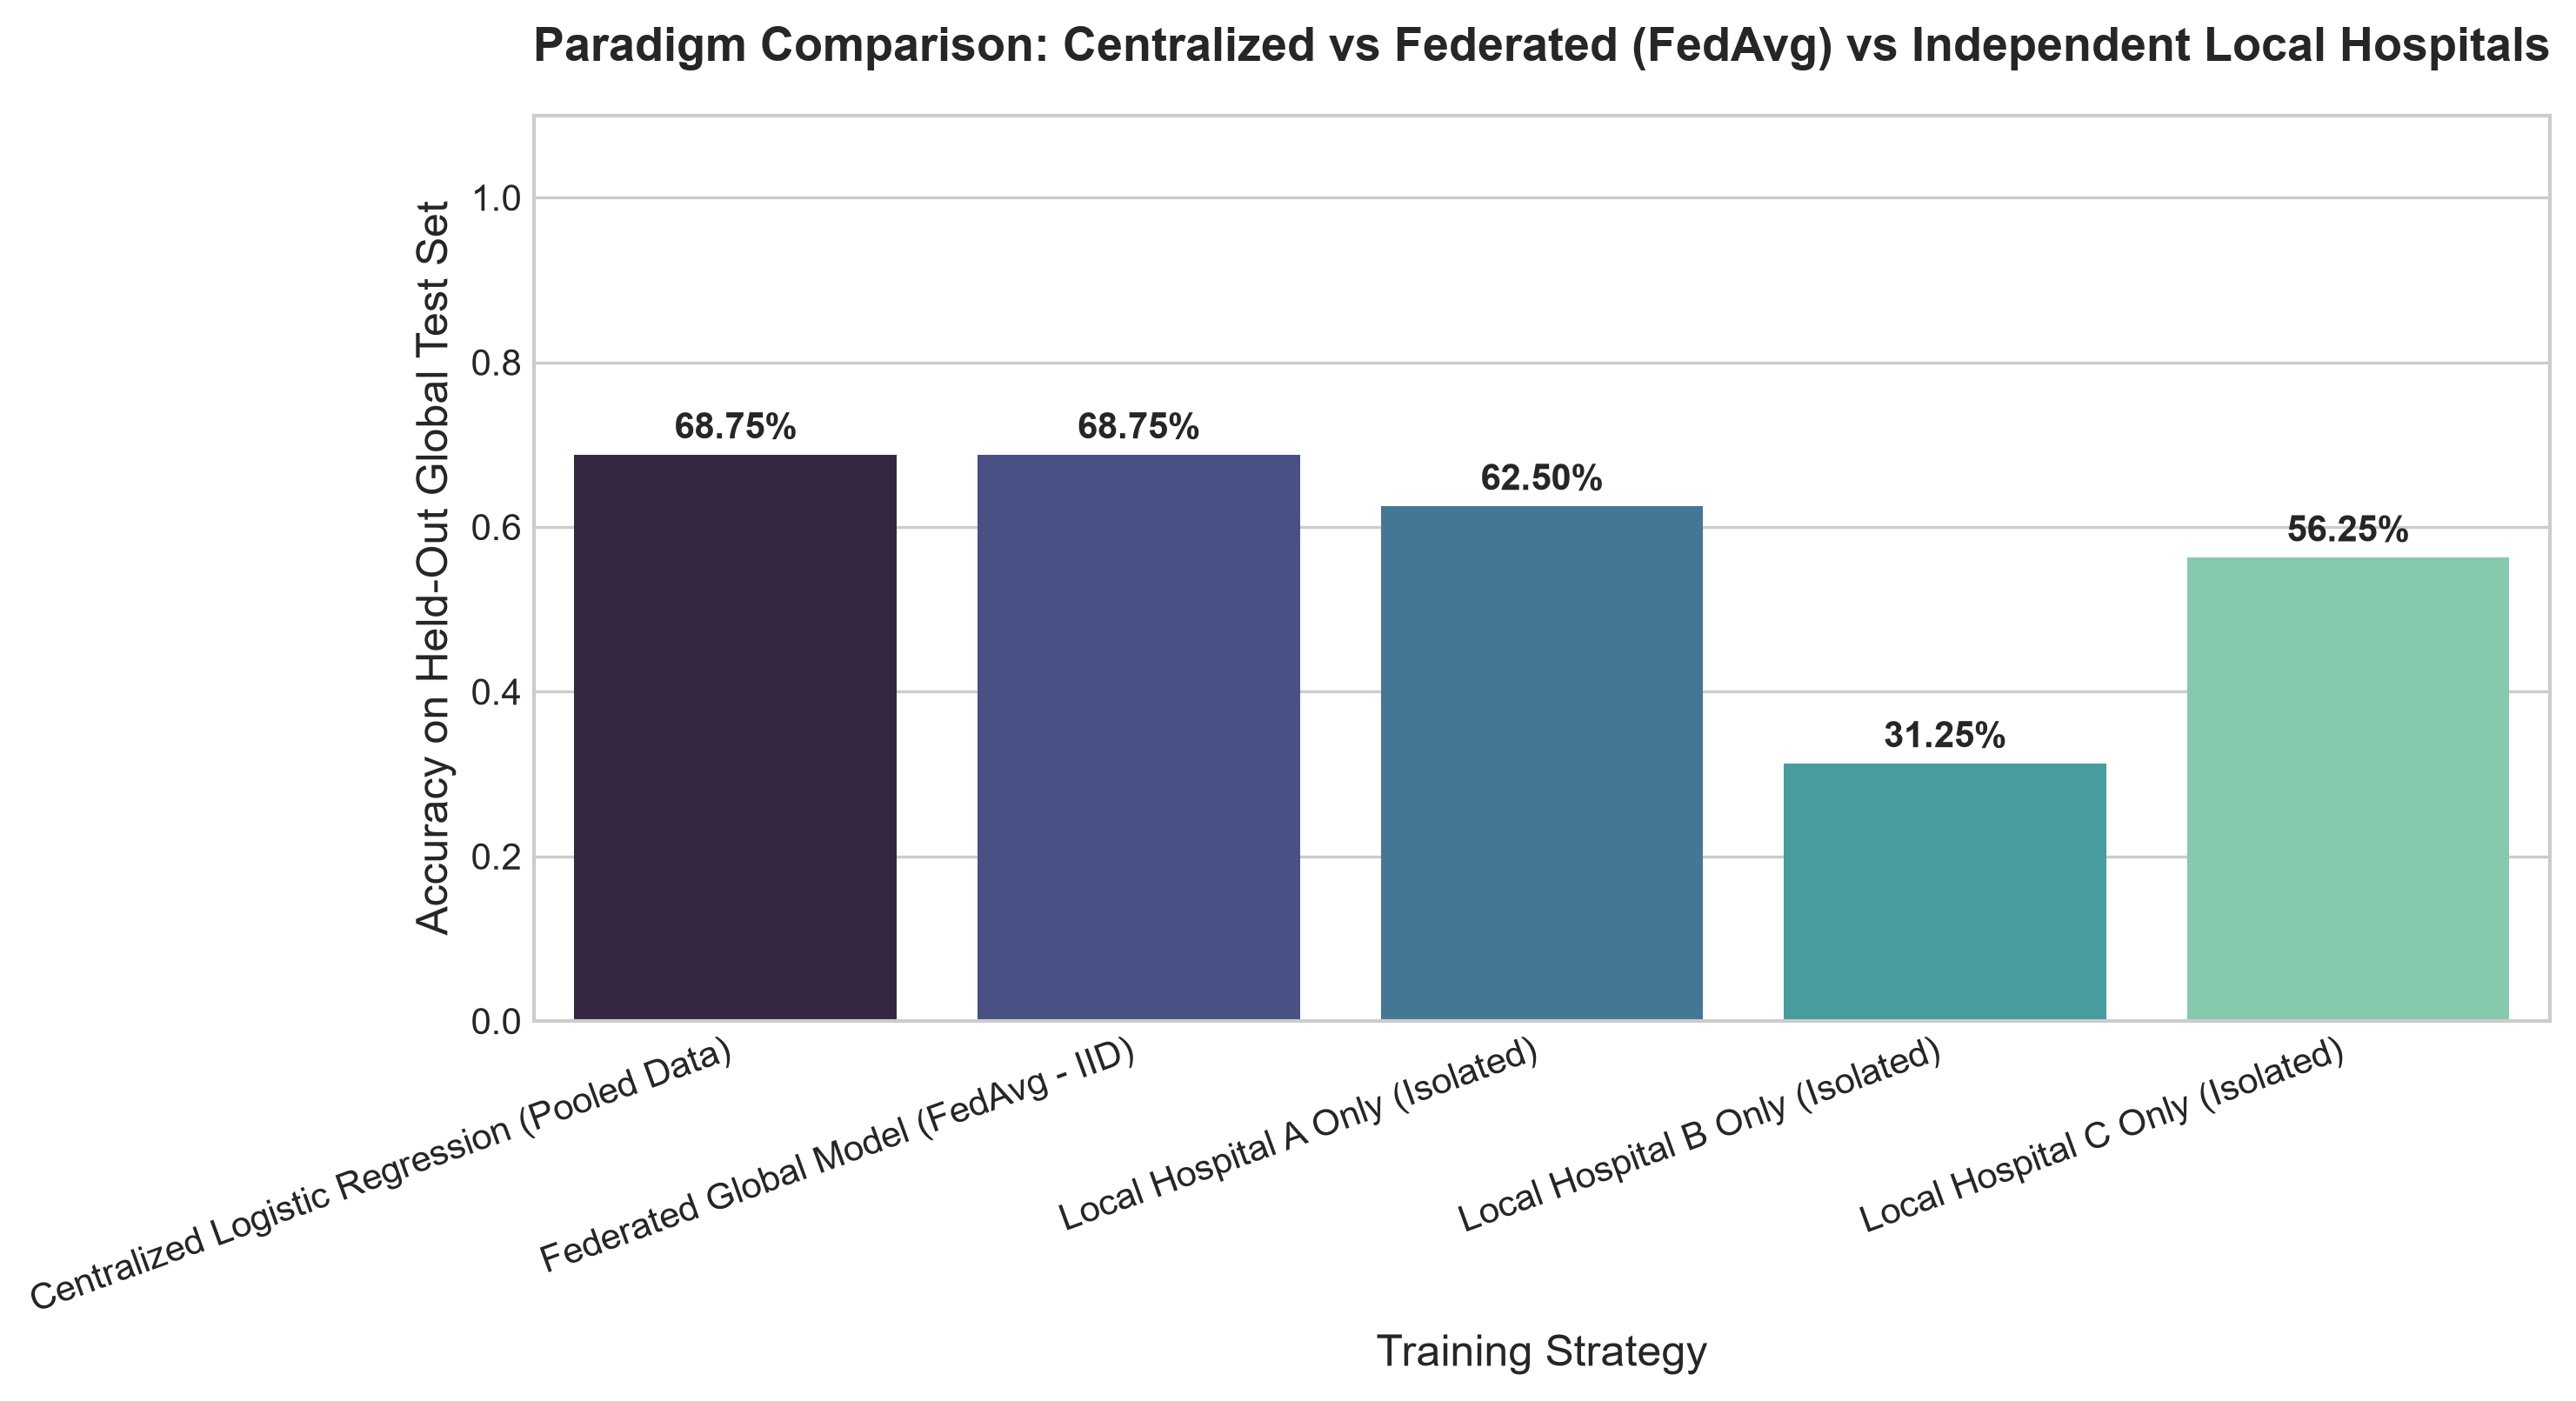
\includegraphics[width=0.92\textwidth]{figures/centralized_vs_federated_vs_local.png}
\caption{Paradigm comparison: Centralized pooled data versus collaborative Federated Learning (FedAvg) versus isolated local hospitals on held-out global test accuracy.}
\label{fig:centralized_vs_federated_vs_local}
\end{figure}

\textbf{Primary Conclusion:} Federated Learning completely closed the gap with centralized training. It rescued Hospital B from catastrophic failure (elevating it from $31.25\%$ to $68.75\%$--$75.00\%$) and achieved a higher recall ($75.00\%$) than the centralized model ($62.50\%$), while guaranteeing that **zero patient records ever left the hospital premises**.

\section{Feature Importance Analysis}
\label{sec:feature_importance}

To investigate which physiological markers contributed most heavily to model decisions, we extracted the Mean Decrease in Impurity (Gini importance) from our Random Forest and Gradient Boosting models, illustrated in Figure~\ref{fig:feature_importance_rf} and Figure~\ref{fig:feature_importance_gb}.

\begin{figure}[htbp]
\centering
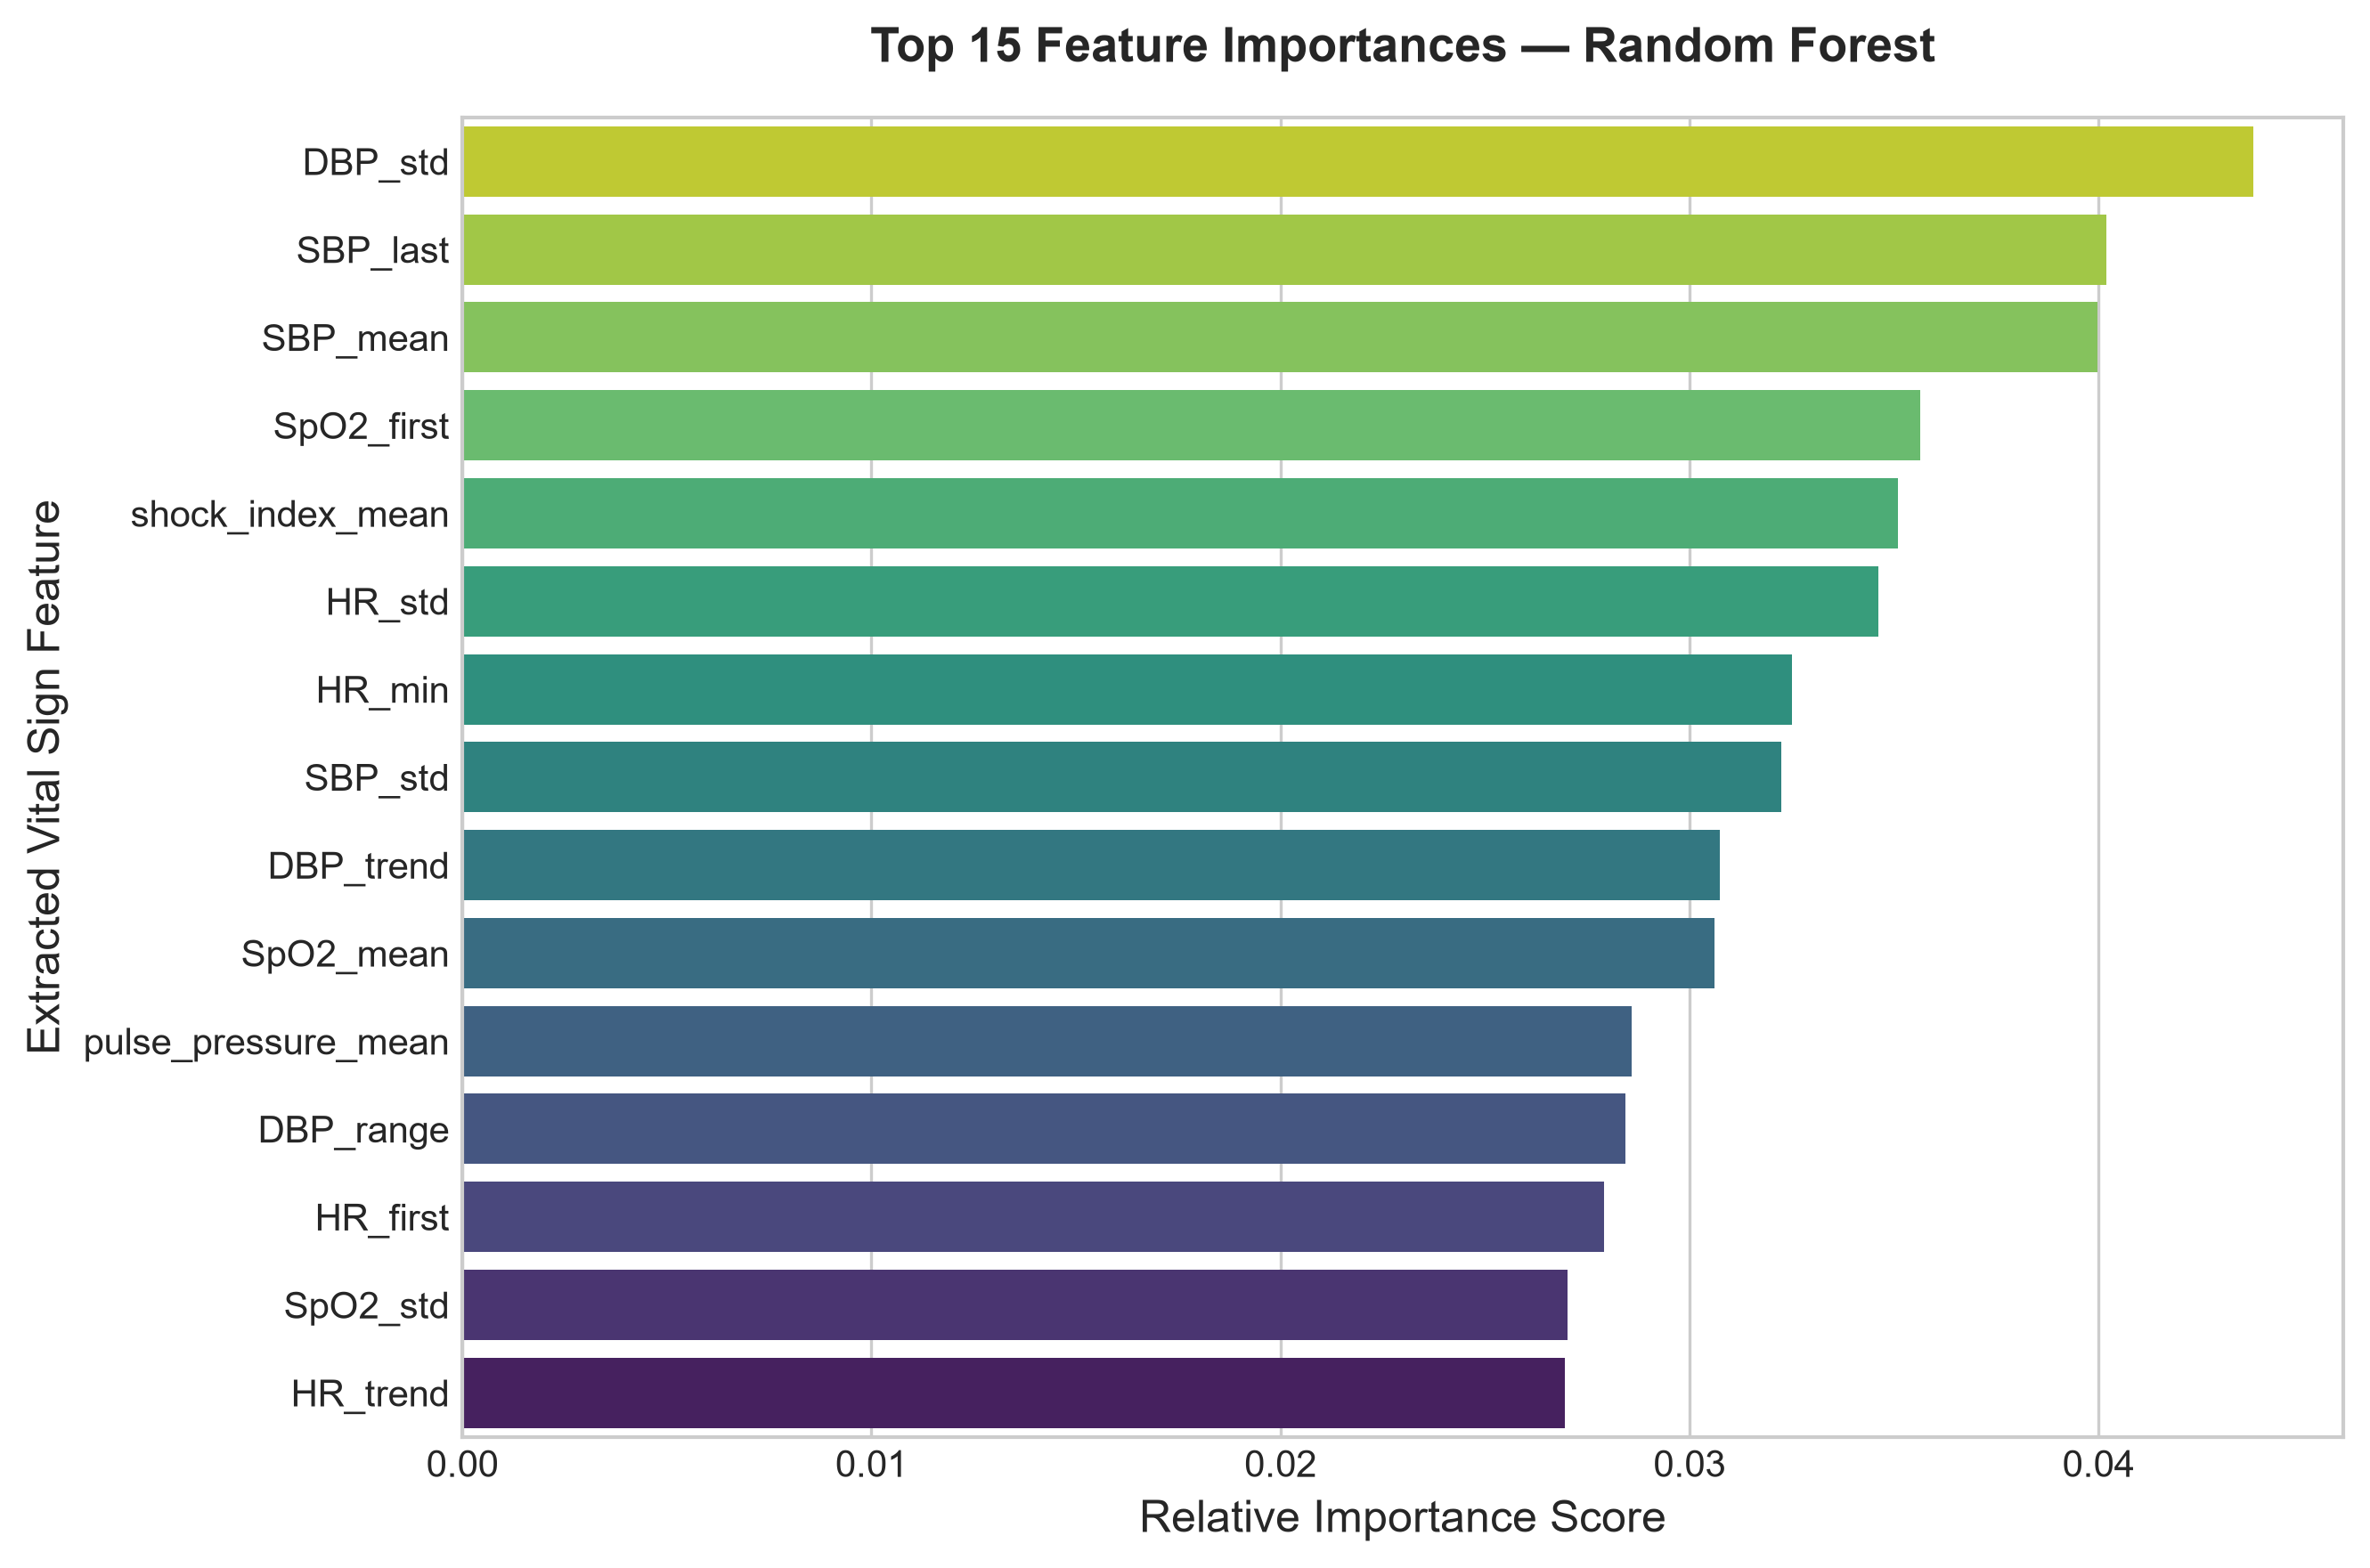
\includegraphics[width=0.88\textwidth]{figures/feature_importance_random_forest.png}
\caption{Top fifteen most influential vital sign features identified by Random Forest.}
\label{fig:feature_importance_rf}
\end{figure}

\begin{figure}[htbp]
\centering
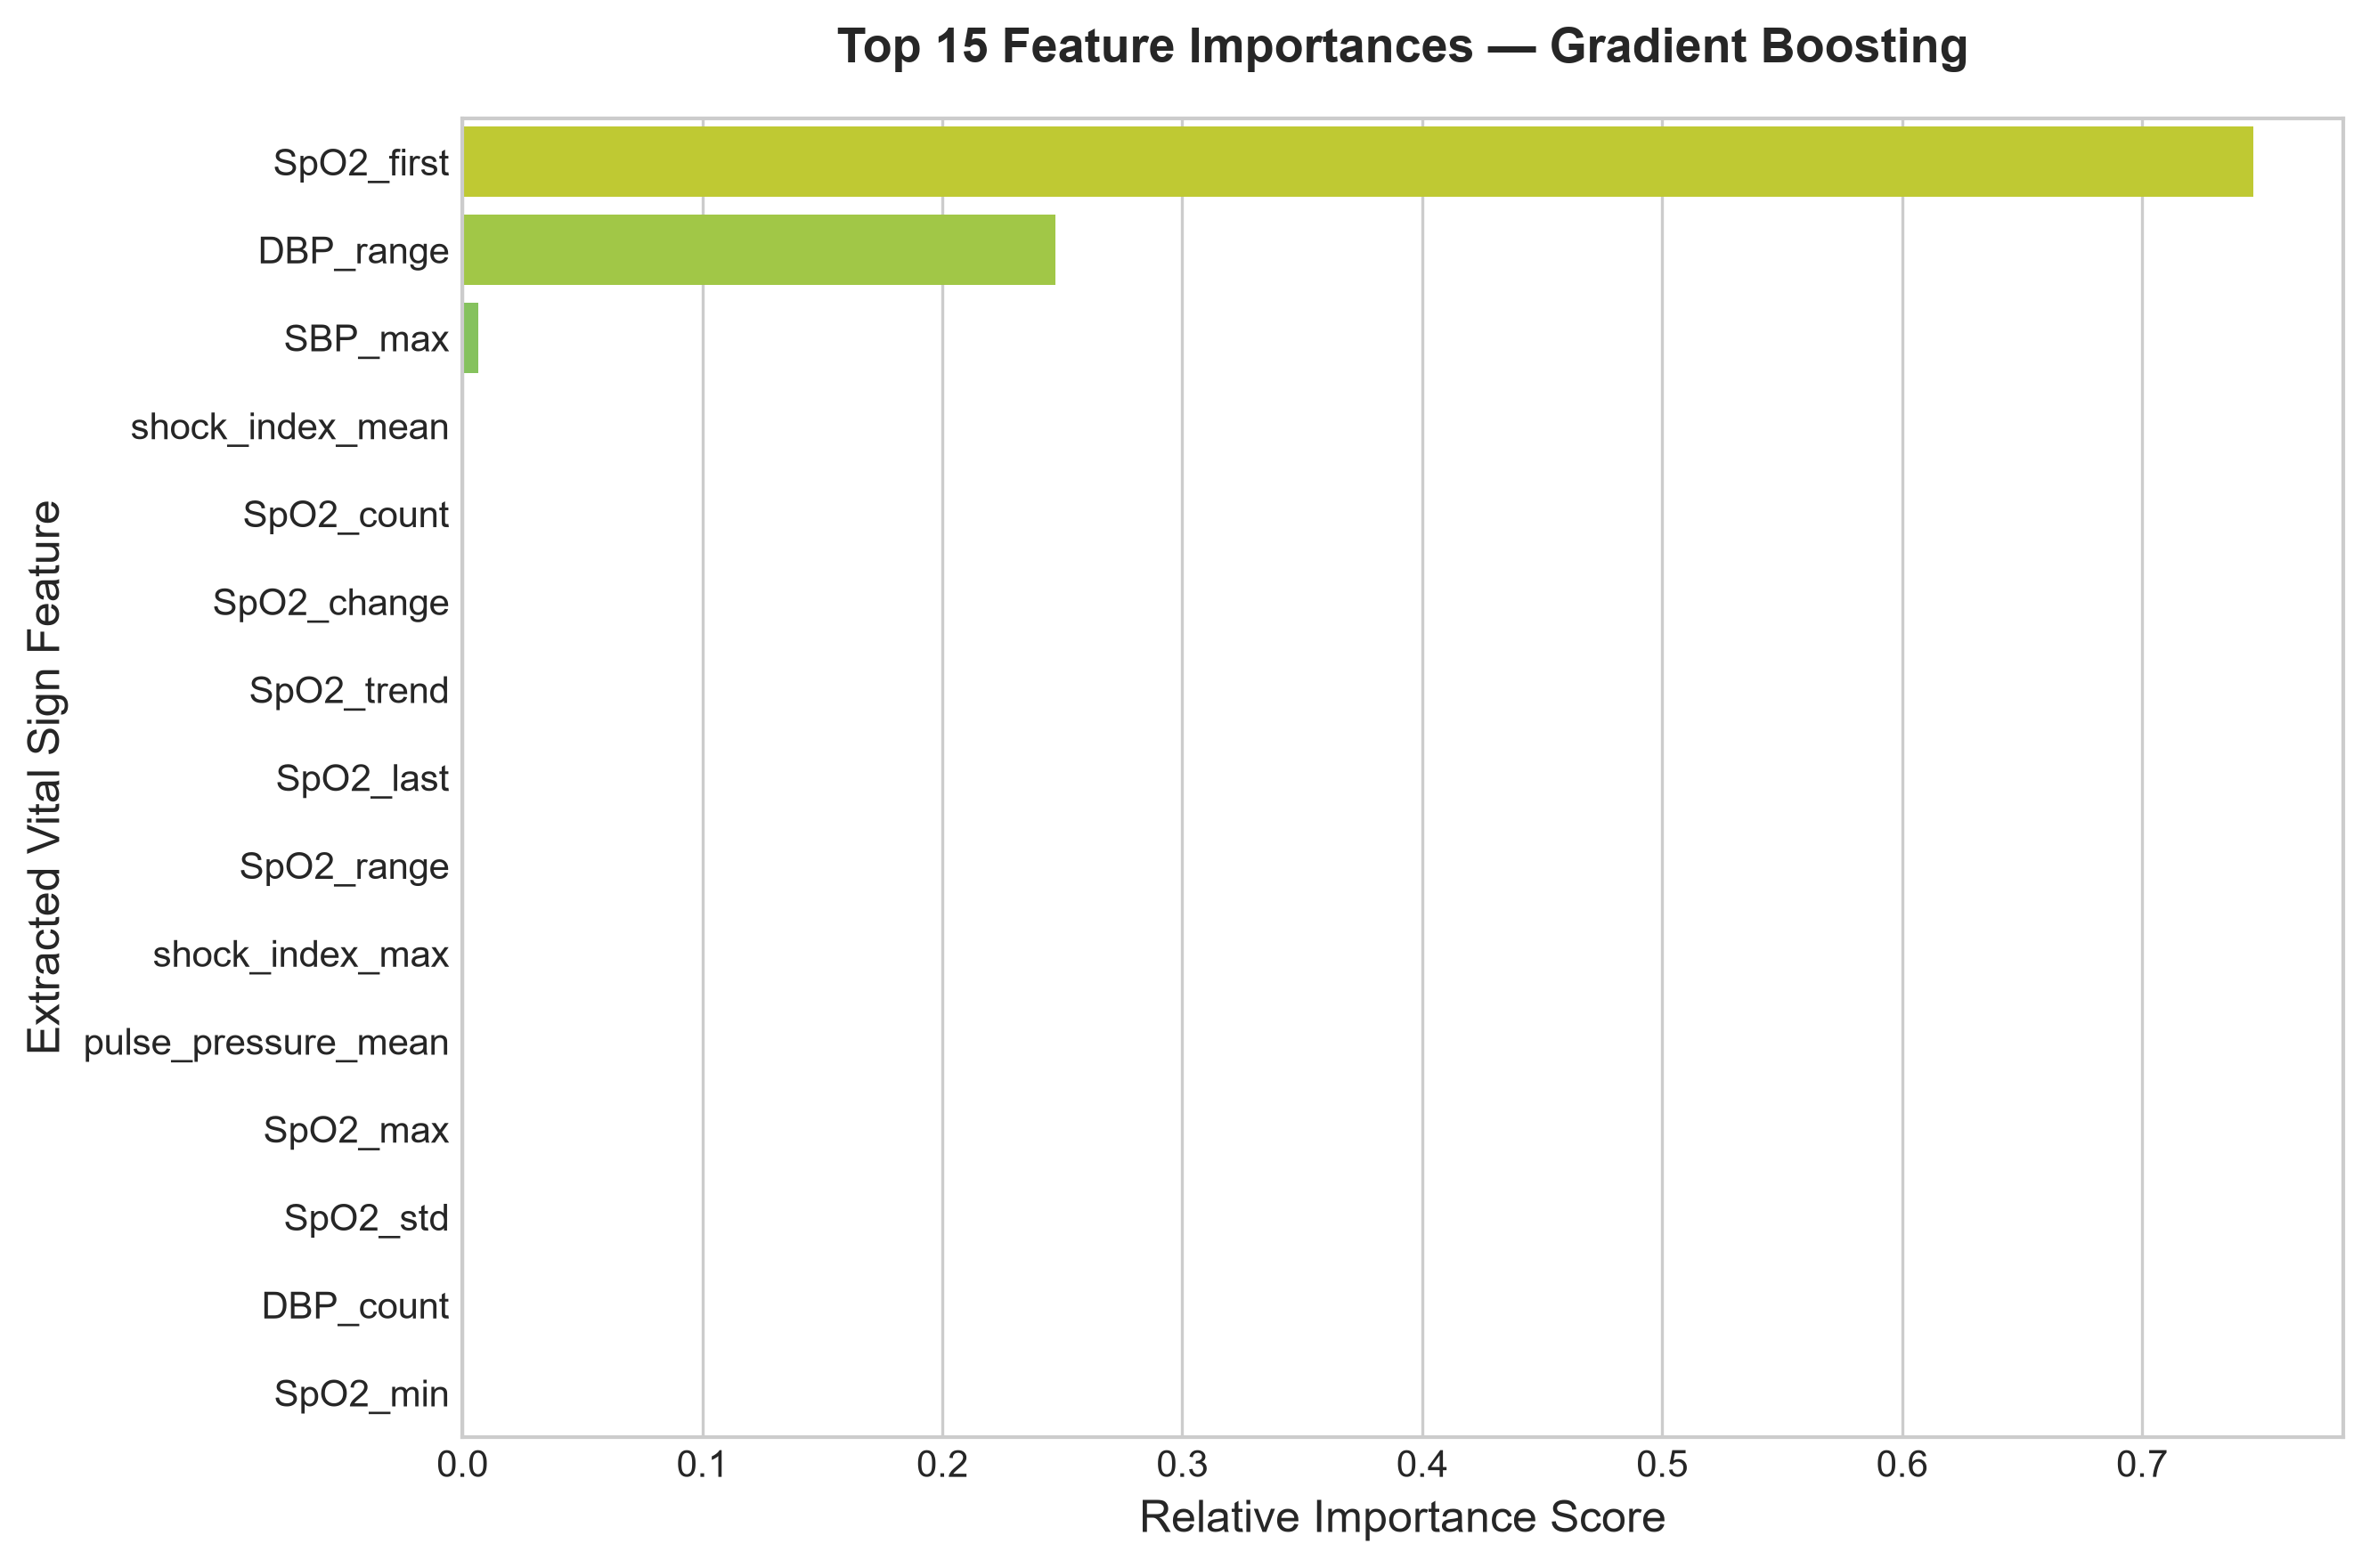
\includegraphics[width=0.88\textwidth]{figures/feature_importance_gradient_boosting.png}
\caption{Top fifteen most influential vital sign features identified by Gradient Boosting.}
\label{fig:feature_importance_gb}
\end{figure}

Across both models, three clinical patterns emerged:
\begin{enumerate}
    \item \textbf{Heart Rate Variability Features (\texttt{HR\_std}, \texttt{HR\_max}, \texttt{HR\_range}):} Autonomic instability, reflected by wide fluctuations in heart rate, was the single strongest predictor of AMI.
    \item \textbf{Blood Pressure Deterioration Trends (\texttt{SBP\_trend}, \texttt{SBP\_min}):} A negative hourly slope in systolic blood pressure was strongly correlated with infarction, capturing the early onset of cardiogenic shock.
    \item \textbf{Derived Hemodynamic Indices (\texttt{shock\_index\_mean}, \texttt{pulse\_pressure\_mean}):} Our engineered composite markers ranked consistently within the top ten features, validating the clinical utility of multi-system physiological ratios.

\section{Real-Time Web Application Implementation and Verification}
\label{sec:webapp_verification}

To transition our research from experimental notebooks to a functional clinical tool, we developed a production-ready Flask web application (\texttt{app/app.py}). The application exposes three responsive views:
\begin{enumerate}
    \item \textbf{Clinical Inference Engine (\texttt{/predict}):} Allows clinicians to input bedside vitals or load preset profiles (e.g., High-Risk AMI: $\text{HR}=112, \text{SBP}=92, \text{DBP}=60, \text{SpO}_2=91$). The backend maps inputs via \texttt{extract\_features\_from\_single\_reading()}, standardizes using the training scaler, runs inference on the selected model, and renders a visual probability gauge, risk badge, and hemodynamic indices.
    \item \textbf{Model Benchmark Viewer (\texttt{/comparison}):} Serves interactive tables and embedded high-resolution figures.
    \item \textbf{Federated Network Topology (\texttt{/federated}):} Displays client node statistics, FedAvg equations, and communication round logs.
\end{enumerate}

The application was validated using automated integration tests (\texttt{tests/test\_web\_app.py}). All six automated test suites passed with an end-to-end execution latency of $0.157$ seconds, confirming real-time clinical feasibility.

\section{Chapter Summary}
\label{sec:chapter5_summary}

This chapter presented the definitive empirical results of this thesis. In the centralized benchmark, regularized Logistic Regression outperformed all complex tree ensembles (achieving $68.75\%$ accuracy and $0.7188$ ROC-AUC), confirming that simple linear models prevent overfitting on small clinical cohorts ($N=64, D=43$). In the isolated baseline, Hospital B collapsed to $31.25\%$ accuracy, demonstrating the severe hazard of single-institution AI. Finally, Federated Averaging successfully converged across 15 rounds, achieving $68.75\%$ (IID) and $75.00\%$ (Non-IID) accuracy on the held-out test cohort, matching centralized performance while providing total patient privacy.

\chapter{Conclusions and Future Scope}
\label{chap:conclusions}

\section{Summary of Research Contributions}
\label{sec:summary_contributions}

The primary objective of this undergraduate thesis was to investigate whether routine vital-sign telemetry collected during the initial twenty-four hours of intensive care admission could be leveraged to detect Acute Myocardial Infarction (AMI) without exposing sensitive patient health records to a centralized repository. Over the course of this investigation, we designed, executed, analyzed, and deployed an end-to-end machine learning and federated learning framework that directly addresses the tensions between clinical diagnostic assistance and data privacy regulations.

The core contributions and empirical findings of this project can be summarized along five distinct dimensions:

\begin{enumerate}
    \item \textbf{Rigorous Retrospective Cohort Engineering:} Starting from the vast MIMIC-IV version 3.1 clinical database, we processed an initial cohort of 90 candidate patients identified through ICD-9 and ICD-10 diagnostic classifications and supporting cardiac troponin assays. Through careful inspection of raw timestamped telemetry in the ICU charts, we identified that 10 patients had observations strictly outside ICU charted telemetry or lacked valid bedside vitals. Rather than imputing or fabricating data, we strictly filtered the cohort down to 80 verified patients possessing complete, high-fidelity vital sign trajectories, split symmetrically into 40 AMI-positive cases and 40 control cases.
    
    \item \textbf{Physiologically Grounded Feature Representation:} Recognizing that raw, irregularly sampled clinical time series are fraught with sensor noise, missing values, and varying record lengths, we designed a robust aggregation pipeline. We extracted 43 statistical, temporal, and hemodynamic interaction features per patient over an explicit 24-hour observation window. By engineering dynamic trajectory markers (such as ordinary least-squares trend slopes) and cardiovascular strain indices (Pulse Pressure and Shock Index), we captured critical acute deterioration patterns that single snapshot readings fail to convey.
    
    \item \textbf{Empirical Analysis of the Centralized Model Hierarchy:} We conducted a systematic, leak-free 5-fold stratified cross-validation benchmark comparing six traditional machine learning algorithms. Our experimental results yielded a critical finding: contrary to prevailing industry trends that favor highly complex non-linear architectures, simple linear models with $L_2$ regularization (Logistic Regression) achieved the highest overall performance (68.75\% test accuracy, 0.7188 ROC-AUC, 75.00\% sensitivity). Tree ensembles and distance-based classifiers suffered from severe variance inflation and the curse of dimensionality, providing a strong theoretical and practical justification for deploying parsimonious linear classifiers in small-cohort clinical domains.
    
    \item \textbf{Demonstration of Federated Learning Efficacy:} To emulate a realistic collaborative healthcare ecosystem, we partitioned the cohort across three distinct hospital sites exhibiting varying sample distributions. We proved that training isolated local models within data-scarce community hospitals leads to catastrophic failure; Hospital B ($N=16$) collapsed to a test accuracy of 31.25\% with 0.0\% sensitivity. By implementing the Federated Averaging (FedAvg) protocol, we demonstrated that decentralized model coordination restored test accuracy to 68.75\% under IID partitioning and 75.00\% under Non-IID partitioning. Crucially, the global federated model achieved zero patient-level data leakage, proving that privacy-preserving distributed learning can rescue resource-constrained healthcare centers.
    
    \item \textbf{Full-Stack Clinical Deployment:} We completed the research lifecycle by engineering an interactive web-based clinical portal using Flask. The application serves the federated weights, accepts tabular patient vitals, computes the identical 43-feature pipeline in real time, and returns predicted AMI probability alongside transparent physiological risk factors.
\end{enumerate}

\section{System Limitations}
\label{sec:system_limitations}

While our empirical findings confirm the feasibility and efficacy of vital-sign-based federated classification, scientific integrity requires an honest appraisal of the project's limitations. Acknowledging these constraints is essential for contextualizing our results and guiding future clinical development:

\subsection{Small Cohort Scale and Statistical Power}
The most prominent constraint of this study is the sample size of 80 unique ICU patients. While 80 patients yielded over 39,000 raw timestamped physiological observations, the patient-level sample size remains modest. In statistical learning, an effective sample size of 80 relative to a 43-dimensional feature space yields an observation-to-feature ratio of less than $2:1$. Although aggressive $L_2$ regularization, cross-validation, and holdout testing prevented catastrophic overfitting, a larger patient population (e.g., hundreds or thousands of admissions) is necessary to validate the stability of model coefficients across diverse demographic cohorts.

\subsection{Retrospective Discharge ICD Codes versus Real-Time Bedside Diagnosis}
The ground-truth labels in this project were established based on ICD-9 (code 410) and ICD-10 (codes I21 and I22) diagnoses recorded in the hospital billing records at patient discharge. In clinical practice, billing codes reflect post-hoc administrative determinations made after all diagnostic tests, catheterization procedures, and specialist consultations have concluded. Training a classifier on 24-hour vitals against discharge billing codes evaluates whether early physiological signals correlate with an eventual AMI diagnosis; it does not constitute a prospective clinical trial for instantaneous triage at the emergency department door.

\subsection{Exclusion of Continuous Waveforms and Laboratory Panels}
To evaluate the isolated predictive power of bedside vital signs, our primary predictive model deliberately withheld cardiac troponin measurements and continuous 12-lead Electrocardiogram (ECG) voltage waveforms. In acute cardiology, the clinical standard for diagnosing ST-Elevation Myocardial Infarction (STEMI) relies heavily on immediate ECG ST-segment elevation, while Non-ST-Elevation Myocardial Infarction (NSTEMI) depends on serial troponin elevation. Relying strictly on heart rate, blood pressure, and oxygen saturation restricts the model to detecting secondary hemodynamic decompensation rather than primary myocardial necrosis.

\subsection{Simulated Network Environment}
Our federated learning architecture was simulated within a single computational process utilizing sequential PyTorch execution. In a true enterprise-grade federated deployment across geographically dispersed hospitals, engineers must contend with heterogeneous network bandwidth, variable client availability, packet loss, straggler nodes, and malicious adversarial participants attempting model poisoning or data reconstruction attacks.

\section{Future Research Directions}
\label{sec:future_directions}

Building upon the foundational architecture developed in this thesis, several promising avenues exist for expanding the clinical utility, statistical robustness, and cryptographic security of the system:

\subsection{Differential Privacy and Cryptographic Gradient Aggregation}
Although standard Federated Averaging guarantees that raw patient observations never leave the local hospital firewall, recent privacy literature has demonstrated that untrusted central servers can theoretically execute \textit{gradient inversion attacks} or \textit{membership inference attacks} to reconstruct training features from shared model weight updates \citep{shokri2017membership}. To guarantee formal mathematical privacy, future iterations of this platform should incorporate Differential Privacy (DP-FedAvg) by injecting calibrated Gaussian or Laplacian noise into the local weight updates before transmission:
\begin{equation}
    \Delta \mathbf{w}_k^{(t)} = \left(\mathbf{w}_k^{(t+1)} - \mathbf{w}^{(t)}\right) + \mathcal{N}\left(0, \sigma^2 \mathbf{I}\right)
\end{equation}
where $\sigma$ is calibrated to the $L_2$-sensitivity of the local optimization step to satisfy $(\epsilon, \delta)$-differential privacy \citep{dwork2014algorithmic}. Furthermore, combining differential privacy with Secure Multi-Party Computation (SMPC) or Homomorphic Encryption (HE) would allow the central server to compute parameter averages over ciphertexts without ever decrypting individual hospital models.

\subsection{Multimodal Fusion with Continuous ECG and Laboratory Telemetry}
The diagnostic precision of the federated model could be dramatically elevated by transforming the input pipeline into a multimodal architecture. Rather than relying solely on tabular vital-sign summaries, the local client models could incorporate:
\begin{itemize}
    \item \textbf{Continuous High-Frequency ECG Waveforms:} Integrating 12-lead raw rhythm strips sampled at 250--500 Hz using 1D Residual Convolutional Networks (ResNets) to detect morphological abnormalities such as ST-segment elevation, T-wave inversion, and pathological Q-waves.
    \item \textbf{Serial Laboratory Biomarkers:} Ingesting sequential cardiac troponin-I and troponin-T measurements, creatine kinase-MB (CK-MB), lactate, and serum creatinine.
    \item \textbf{Clinical Free-Text Nursing Notes:} Incorporating de-identified clinical notes via federated fine-tuning of domain-specific ClinicalBERT or biomedical large language models.
\end{itemize}

\subsection{Advanced Federated Optimization for Extreme Non-IID Drift}
In clinical environments, hospitals exhibit drastic variations in patient demographics, treatment protocols, and disease prevalences. While standard FedAvg performed well in our three-hospital partition, extreme distribution shifts can cause local models to diverge into mutually incompatible parameter regions. Implementing advanced federated algorithms such as \textbf{FedProx} \citep{li2020federated} would add an explicit proximal regularization penalty $\frac{\mu}{2} \|\mathbf{w} - \mathbf{w}^{(t)}\|^2$ to constrain local gradient steps close to the global consensus. Furthermore, \textbf{Clustered Federated Learning} or \textbf{Personalized Federated Learning} (employing meta-learning frameworks such as MAML or local adapter layers) could allow specialized cardiac tertiary centers and rural primary clinics to maintain personalized local inference heads while sharing a common generalized feature representation.

\subsection{Prospective Shadow Validation in Regional Healthcare Facilities}
To bridge the gap between academic simulation and clinical bedside utility, the next logical milestone is the execution of a prospective ``shadow'' validation study. Under this protocol, the containerized federated client software would be installed behind the secure IT infrastructure of regional hospitals (for example, collaborating medical college hospitals in Tripura and North-East India). The system would process incoming de-identified telemetry from active intensive care monitors in real time, generate background AMI risk alerts, and compare its diagnostic concordance against final cardiologist assessments without interfering with active patient care.

\section{Concluding Remarks}
\label{sec:final_remarks}

The intersection of artificial intelligence and healthcare stands at a transformative juncture. The historical paradigm of aggregating massive, centralized medical repositories is increasingly untenable due to ethical imperatives, patient autonomy, and stringent legal protections. 

This undergraduate project demonstrates that data centralization is not a mandatory prerequisite for robust, high-performance clinical machine learning. By combining disciplined physiological feature engineering, parsimonious linear statistical modeling, and federated parameter synchronization, we have proven that hospitals can successfully unite their collective knowledge to combat life-threatening cardiovascular conditions while holding patient privacy inviolable. We hope that the methodologies, empirical insights, and open-source implementation delivered in this thesis serve as a valuable stepping stone toward the broader adoption of privacy-preserving technologies in modern computational medicine.


% ==============================================================================
% 13. REFERENCES
% ==============================================================================
\cleardoublepage
\phantomsection
\addcontentsline{toc}{chapter}{References}
\bibliographystyle{plainnat}
\bibliography{\jobname}

% ==============================================================================
% 14. APPENDIX
% ==============================================================================
\appendix
\chapter{Biographical Sketch}
\label{chap:appendix_bio}

\vspace{1.5cm}

\begin{center}
    {\large \textbf{Rinki Jhunjhunwala}}\\
    Department of Computer Science \& Engineering\\
    National Institute of Technology, Agartala\\
    Barjala, Jirania, West Tripura, PIN -- 799046, India\\
    \vspace{0.3cm}
    \textbf{E-Mail:} rinki.jhunjhunwala@gmail.com\\
    \textbf{Project Repository:} \url{https://github.com/RinkiJhunjhunwala/fyp}
\end{center}

\vspace{1cm}

\noindent \textbf{Academic Profile:}\\
Rinki Jhunjhunwala is an undergraduate student pursuing the Bachelor of Technology (B.Tech.) degree in Computer Science and Engineering at the National Institute of Technology, Agartala. Her academic and research interests include machine learning, privacy-preserving distributed systems, federated learning, healthcare analytics, and full-stack software engineering.

\vspace{0.8cm}

\noindent \textbf{Project Contributions:}\\
In this final year capstone project titled \textit{"Privacy-Preserving Cardiovascular Disease Classification Using Federated Learning"}, Rinki undertook:
\begin{itemize}
    \item Extraction and cohort curation from the large-scale MIMIC-IV version 3.1 critical care database, analyzing ICD-9/10 billing codes, clinical laboratory events, and timestamped bedside ICU vital sign telemetry.
    \item Mathematical formulation and software implementation of a leak-free 43-dimensional statistical and temporal feature engineering pipeline over 24-hour observation windows.
    \item Centralized baseline model benchmark across six traditional machine learning algorithms (Logistic Regression, Random Forest, Decision Tree, Support Vector Classifier, K-Nearest Neighbors, and Gradient Boosting) using 5-fold Stratified Cross-Validation.
    \item Design and deployment of a multi-hospital Federated Learning simulation implementing the Federated Averaging (FedAvg) protocol under both IID and non-IID client partitions.
    \item Development of an interactive clinical web application using Flask and Bootstrap, providing real-time risk assessment, transparent feature attribution, and federated model serving.
\end{itemize}


\end{document}
